% ============================================================================
% Accessibility
% ============================================================================
\DocumentMetadata{
  lang = en-US, 
  pdfstandard = ua-2, 
  tagging = on, 
  tagging-setup = {math/setup=mathml-SE}
}

% ============================================================================
% Document Properties - used on title slide and PDF metadata fields
% ============================================================================
\def\PresTitle{Electricity and Electrical Safety}  % Required - top line of title slide
\def\PresSubtitle{Programmable Logic Controllers}         % Optional - second line
\def\PresAuthor{Brad Peirson}               % Required - below dividing line
\def\PresInstitute{College of Information Technology and Engineering}       % Optional
\def\PresDate{}                             % Optional
\def\PresKeywords{}                         % Optional - used for hyperref

% ============================================================================
% Presentation Formatting
% ============================================================================
% ============================================================================
% Class Declaration
% ============================================================================
\documentclass[
        mode = handout,     % Projector = one bullet at a time, Handout = all
        font-size=14pt,     % Only accepts 9, 10, 12, 14, 17, 20
        pdfusetitle         % Pulls \title property from document
    ]
    {ltx-talk}              % ltx-talk class

% ============================================================================
% Custom Colors
% ============================================================================
\usepackage[table]{xcolor}
% Colors from the Baker College Style Guide
\definecolor{BakerADARed}{RGB}{231, 0, 46}
\definecolor{HoneyYellow}{RGB}{255, 196, 0}
\definecolor{UpNorthGreen}{RGB}{114, 191, 68}
\definecolor{LakeBlue}{RGB}{134, 183, 227}
\definecolor{BakerADI}{RGB}{58, 98, 170}
\definecolor{BakerCIM}{RGB}{217, 35, 47}
\definecolor{BakerBlack}{RGB}{31, 34, 40}
\definecolor{BakerWhite}{RGB}{255, 255, 255}
\definecolor{BakerRed}{RGB}{239, 0, 48}
\definecolor{Abbey}{RGB}{80, 82, 88}
\definecolor{RollingStone}{RGB}{121, 124, 126}
\definecolor{HitGray}{RGB}{165, 169, 172}
\definecolor{Iron1}{RGB}{201, 206, 209}
\definecolor{Iron}{RGB}{222, 225, 226}
\definecolor{BlackHaze1}{RGB}{237, 240, 240}
\definecolor{BlackHaze}{RGB}{245, 247, 247}

% ============================================================================
% Document Data
% ============================================================================
\title{\PresTitle}
\author{\PresAuthor}
\institute{\PresInstitute}
\date{\PresDate}

%Set up the hyperlink colors
\hypersetup{colorlinks,
    linkcolor=BakerBlack,
    urlcolor=BakerADARed,
    pdfauthor = {\PresAuthor},
    %pdftitle = {\PresentationTopic},   % Title is pulled directly
    pdfsubject = {\PresSubtitle},
    pdfkeywords = {\Keywords},
    pdfcreator = {LaTeX with hyperref package},
    pdfproducer = {LuaLaTeX}
    }

% Map your custom style guide colors to the progress bar aliases
\colorlet{pbcomplete}{BakerADARed}
\colorlet{pbincomplete}{Iron}

\usepackage[most]{tcolorbox}

% ============================================================================
% Footer Format
% ============================================================================
\EditInstance{footer}{std}{
  color         = Abbey,
  separator     = \hfill,
  element-order = {title, institute, framenumber},
  right-hspace  = 3mm,
  left-hspace   = 3mm,
}

% \DeclareInstance{footer}{empty}{
%   element-order = {}
% }

% ============================================================================
% Progress Bar Toggles & Helper Macros
% ============================================================================
\usepackage{xfp}        % Needed for floating point math
\newif\ifprogressbar    % Used to determine whether or not to show the bar
\progressbartrue        % Set the bar to true at the start

% Helper macro to automatically turn off the progress bar inside title/section frames
\newcommand{\makeblindframe}[1]{%
  \progressbarfalse
  #1%
  \progressbartrue
}

% ============================================================================
% Custom Page Formats
% ============================================================================
\let\oldmaketitle\maketitle         % Backup the original maketitle command
\let\oldsection\section             % Backup the original section command
\let\oldsubsection\subsection       % Backup the original subsection command

\makeatletter
\renewcommand{\maketitle}{%
\makeblindframe{%
  \disableglobalbackground
  \slidebackground{BakerPresentation_TitleBackground}%
  \color{white}%
  %\UseInstance{footer}{wallpaper}
  \begin{frame}[wallpaper]
    \vspace*{1in}%
      \begin{tcolorbox}[
          enhanced,
          colback=black,       
          colframe=black,      
          opacityfill=0.25,       
          arc=6pt,                
          boxrule=0pt,            
          left=20pt, right=20pt,  
          top=20pt, bottom=20pt,
          width=0.80\textwidth,   
          halign=left             
      ]
          \color{white}%
          % Title (Always visible)
          {\large\bfseries\sffamily \@title}\\[0.5em]%
          
          % Conditional Subtitle
          \ifx\PresSubtitle\empty
          \else
            {\normalsize\sffamily \PresSubtitle}\\[0.5em]%
          \fi
          
          % High-contrast divider line
          {\color{white!80}\rule{0.3\textwidth}{0.8pt}}\\[0.5em]%
          
          % Author (Always visible)
          {\small\sffamily \@author}\\%
          
          % Conditional Institute
          \ifx\PresInstitute\empty
          \else
            {\small\sffamily \PresInstitute}\\%
          \fi
          
          % Conditional Date
          \ifx\PresDate\empty
          \else
            {\small\sffamily \@date}\\%
          \fi
      \end{tcolorbox}%
      \vfill     
  \end{frame}%
  \enableglobalbackground{BG}%
  \color{black}%
  %\UseInstance{footer}{std}
}%
}
\makeatother

% Create a variable container to hold the current section title
\newcommand{\currentsectiontitle}{}

% Redefine \section to take 1 argument (the title)
\renewcommand{\section}[1]{%
\makeblindframe{%
  \renewcommand{\currentsectiontitle}{#1}%
  \disableglobalbackground
  \slidebackground{BakerPresentation_SectionBackground}%
  \begin{frame}
    \vfill
    %\vspace*{0.625in}%
    \begin{tcolorbox}[
        enhanced,
        colback=black,       
        colframe=black,      
        opacityfill=0.25,       
        arc=6pt,                
        boxrule=0pt,            
        left=20pt, right=20pt,  
        top=20pt, bottom=20pt,
        width=0.80\textwidth,   
        halign=left             
    ]
        \color{white}%
        {\large\bfseries\sffamily #1}\\[0.5em]%   
    \end{tcolorbox}%
    \vfill 
  \end{frame}%
  \oldsection{#1}%
  \enableglobalbackground{BG}%

  % This will be used for an auto TOC at every section
  % Right now ltx-talk TOC is still in development
  % Once it comes a little further along this can be used
  % \begin{frame}
  %       \frametitle{Section Overview}
  %       \tableofcontents[sections=\thesection]
  %   \end{frame}%
}%
}

% Redefine \subsection to take 1 argument
\renewcommand{\subsection}[1]{%
\makeblindframe{%
  \disableglobalbackground
  \slidebackground{BakerPresentation_SectionBackground}%
  \begin{frame}
    \vfill
    %\vspace*{0.25in}% 
    \begin{tcolorbox}[
        enhanced,
        colback=black,       
        colframe=black,      
        opacityfill=0.25,       
        arc=6pt,                
        boxrule=0pt,            
        left=20pt, right=20pt,  
        top=20pt, bottom=20pt,
        width=0.80\textwidth,   
        halign=left             
    ]
        \color{white}%
        {\large\bfseries\sffamily\currentsectiontitle}\\[0.5em]%
        {\normalsize\sffamily #1}%
    \end{tcolorbox}%
    \vfill 
  \end{frame}%
  \oldsubsection{#1}%
  \enableglobalbackground{BG}%
}%
}

%Set the fonts to use NeueHaas Grotesk
\setsansfont{NHaasGroteskTXPro-}[
    Path=../../NeueHaasGroteskFiles/,
    Scale=1.0,
    Extension = .ttf,
    UprightFont=*55Rg,
    BoldFont=*75Bd,
    ItalicFont=*56It,
    BoldItalicFont=*76BdIt
    ]

% Force the document default family to Sans-Serif
\renewcommand{\familydefault}{\sfdefault}

\usepackage{mathtools} % Load BEFORE unicode math settings
\setmathfont{Fira Math}[Scale=MatchLowercase] 

% 1. Turn global background ON
\newcommand{\enableglobalbackground}[1]{%
  \AddToHook{shipout/background}[mybg]{%
    \put(0, -\paperheight){%
      \includegraphics[width=\paperwidth, height=\paperheight, artifact]{#1}%
    }%
  }%
}

% 2. Turn global background OFF
\newcommand{\disableglobalbackground}{%
  \RemoveFromHook{shipout/background}[mybg]%
}

\newcommand{\slidebackground}[1]{%
  \AddToHookNext{shipout/background}{%
    \put(0, -\paperheight){%
      \includegraphics[width=\paperwidth, height=\paperheight, artifact]{#1}%
    }%
  }%
}

% --- GLOBAL BULLET OVERRIDES ---
\renewcommand{\labelitemi}{\color{BakerBlack}\Large\textbullet}
\renewcommand{\labelitemii}{\color{BakerBlack}\large\textbullet}
\renewcommand{\labelenumi}{\color{BakerBlack}\bfseries\arabic{enumi}.}
\renewcommand{\labelenumii}{\color{BakerBlack}\bfseries\alph{enumii})}

% Global override for ltx-talk slide titles
\EditInstance{frametitle}{header}{
    font = \rule{0pt}{1.5cm}\bfseries\Large,
}

\EditInstance{header}{std}{
    font = \bfseries\huge,
    color = BakerBlack,
}

\usepackage[americanvoltages]{circuitikz}
\usepackage{pgfplots}
\usepackage{pgf-pie}

\usetikzlibrary{
    intersections, 
    fillbetween,
    patterns,
    decorations.pathreplacing,
    decorations.pathmorphing,
    decorations.text,
    decorations.markings,
    arrows.meta,
    arrows,
    shapes,
    shapes.geometric,
    shadows,
    calligraphy,
    backgrounds,
    intersections,
    calc,
    math,
    positioning
    }

\tikzset{middlearrow/.style={
        decoration={markings, 
        mark= at position 0.5 with {\arrow{#1}},
        },
        postaction={decorate}
    }
}

\pgfplotsset{compat=1.18}

\pgfdeclarelayer{ft}
\pgfdeclarelayer{bg}
\pgfsetlayers{bg, main, ft}

\newcommand{\hexpic}[4][]{%
  \begin{tikzpicture}[baseline=(hex.base)]
    \node (hex) [
      draw=white, 
      minimum size=#2, 
      regular polygon, 
      regular polygon sides=6, 
      rotate=90,
    ] {};
    \begin{scope}
      \clip (hex.corner 1) -- (hex.corner 2) -- (hex.corner 3) -- 
            (hex.corner 4) -- (hex.corner 5) -- (hex.corner 6) -- cycle;
      \node at (hex.center) [#1] {
        \includegraphics[height=#2, alt={#3}]{#4}
      };
    \end{scope}
  \end{tikzpicture}
}

% % ============================================================================
% % Progress Bar Logic 
% % ============================================================================
% \makeatletter               
% \AddToHook{shipout/background}{%
%   \ifprogressbar
%     % Read ltx-talk's internal frame counters safely
%     \edef\currentframe{\@framenumber}%
%     \edef\totalframes{\@totalframes}%
    
%     % Fallback checks: If the document hasn't fully compiled yet, default to 1
%     \ifx\currentframe\empty\def\currentframe{1}\fi
%     \ifx\totalframes\empty\def\totalframes{1}\fi
    
%     % Draw the progress bar if we have a valid total frame count
%     \ifnum\totalframes>1\relax
%       % Compute fraction width: (current - 1) / (total - 1)
%       \edef\pbfraction{\fpeval{(\currentframe - 1) / (\totalframes - 1)}}%
%       \edef\completewidth{\fpeval{\pbfraction * \paperwidth}}%
%       \edef\incompletewidth{\fpeval{\paperwidth - \completewidth}}%
      
%       % Render full-width progress bar at the top edge
%       \put(0cm, -0.1cm){%
%         \color{pbcomplete}\rule{\completewidth pt}{2pt}%
%         \color{pbincomplete}\rule{\incompletewidth pt}{2pt}%
%       }%
%     \fi
%   \fi
% }
% \makeatother

\pretocmd{\tableofcontents}{\begin{minipage}{\textwidth} \linespread{1.4}}{}{}
\apptocmd{\tableofcontents}{\end{minipage}}{}{}

%Biber not functional in ltx-talk as of 2026-05-29
%Package that allows the creation of bibliographies
\usepackage[
    backend=biber,
    style=authoryear,
    sorting=none,
    %entryhead=false
    ]{biblatex}

%Load the bibliography file
\addbibresource{../../reference.bib}

\defbibheading{bibslide}{References}

\newcolumntype{L}[1]{>{\raggedright\let\newline\\\arraybackslash\hspace{0pt}}m{#1}}
\newcolumntype{C}[1]{>{\centering\let\newline\\\arraybackslash\hspace{0pt}}m{#1}}
\newcolumntype{R}[1]{>{\raggedleft\let\newline\\\arraybackslash\hspace{0pt}}m{#1}}

%All of the graphics are in a seperate folder, this makes it so the folder doesn't have to be repeated every time
\graphicspath{
  {../../assets/images}
  {../../assets/diagrams}
  {../../assets/plots}
}

\makeatletter
% New counter to hold the custom "max frames" for the progress bar
\newcommand{\pb@maxtotal}{1}

% Read the custom total from the .aux file if it exists
\AtBeginDocument{%
  \ifdefined\pb@storedtotal
    \let\pb@maxtotal\pb@storedtotal
  \else
    % Fallback to standard total if our custom hook hasn't run yet
    \edef\pb@maxtotal{\@totalframes}%
  \fi
}

% Custom Appendix command that caps the progress bar and turns it off
\newcommand{\talkappendix}{%
  % 1. Write the CURRENT frame number to the .aux file as the progress total
  \immediate\write\@auxout{\string\gdef\string\pb@storedtotal{\@framenumber}}%
  % 2. Turn off the progress bar for all subsequent appendix slides
  \progressbarfalse
}
\makeatother

% ============================================================================
% Progress Bar Logic 
% ============================================================================
\makeatletter               
\AddToHook{shipout/background}{%
  \ifprogressbar
    % Read ltx-talk's internal frame counter safely
    \edef\currentframe{\@framenumber}%
    \edef\totalframes{\pb@maxtotal}% Use our custom max total instead
    
    % Fallback checks: If the document hasn't fully compiled yet, default to 1
    \ifx\currentframe\empty\def\currentframe{1}\fi
    \ifx\totalframes\empty\def\totalframes{1}\fi
    
    % Draw the progress bar if we have a valid total frame count
    \ifnum\totalframes>1\relax
      % Compute fraction width: (current - 1) / (total - 1)
      \edef\pbfraction{\fpeval{(\currentframe - 1) / (\totalframes - 1)}}%
      
      % Guard rails to prevent the bar from overshooting 100% on a first compile
      \ifdim\pbfraction pt>1pt\def\pbfraction{1}\fi 
      
      \edef\completewidth{\fpeval{\pbfraction * \paperwidth}}%
      \edef\incompletewidth{\fpeval{\paperwidth - \completewidth}}%
      
      % Render full-width progress bar at the top edge
      \put(0cm, -0.1cm){%
        \color{pbcomplete}\rule{\completewidth pt}{2pt}%
        \color{pbincomplete}\rule{\incompletewidth pt}{2pt}%
      }%
    \fi
  \fi
}
\makeatother

% 1. Globally shrink all caption components right as the caption engine fires
\AddToHook{cmd/@makecaption/before}{\footnotesize}

% 2. Declare and assign a blank plug to the kernel's caption label socket
\NewSocketPlug{caption/label}{nolabel}{}
\AssignSocketPlug{caption/label}{nolabel}

\usepackage{adjustbox}

\usepackage{amssymb}
\usepackage{amsmath}

\newcommand{\ccwplus}{%
  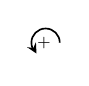
\begin{tikzpicture}[baseline=(char.base)]
    \node(char) at (0,0) {\(\scriptscriptstyle +\)};
    \draw[->, >=stealth, semithick] (0.2,0) arc (0:230:0.18cm);
  \end{tikzpicture}%
}

\usepackage{animate}

\usepackage{calc} % Optional, but helpful for layout

\newcommand{\tikztodo}[3][0.8\textwidth]{%
  \begin{center}
    \fbox{%
      \parbox[c][#2][c]{#1}{%
        \centering
        \textbf{\textcolor{red}{TODO: TikZ Diagram}}\\[0.5em]
        \small #3%
      }%
    }%
  \end{center}%
}

% ============================================================================
% Document Content
% ============================================================================
\begin{document}

\maketitle              % Redefined in the preamble to generate a full frame

\begin{frame}
    \frametitle{Agenda}
    \begingroup
        % Tighten the spacing between paragraphs/TOC lines
        \setlength{\parskip}{0.3em} 
        
        % Optionally tighten the line spacing within an entry
        %\baselineskip=1.2em 
        
        \setcounter{tocdepth}{1} % Show only sections
    \tableofcontents
    \setcounter{tocdepth}{2} % Reset back to default so subsections are tracked
    \endgroup
\end{frame}

\begin{frame}
    \frametitle{Student Learning Outcomes}
    \begin{itemize}[<+- | alert@+>]
        \item[1.]{Create programs in Ladder Logic using the following instructions in an application}
        \item[2.]{Program PLC timers and counters}
    \end{itemize}
\end{frame}

\section{Electricity Review}

\begin{frame}
    \frametitle{Electricity}
    \begin{figure}
        \centering

        \hexpic[]{0.375\linewidth}{A double electric arc from a Tesla coil, electrical experience at the science festival in October 2016 in Le Teil d'Ardèche}{Arc_electrique_double}
        %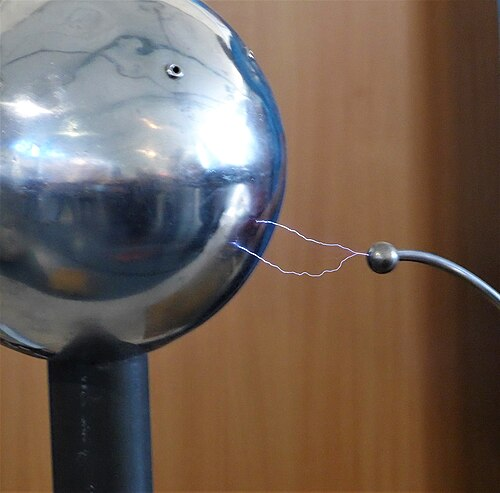
\includegraphics[width=0.375\columnwidth, alt={A double electric arc from a Tesla coil, electrical experience at the science festival in October 2016 in Le Teil d'Ardèche}]{Arc_electrique_double}
        
        {\tiny Attribution: Celeda, \href{https://creativecommons.org/licenses/by-sa/4.0}{CC BY-SA 4.0}, via \href{https://commons.wikimedia.org/wiki/File:Arc_\%C3\%A9lectrique_double.jpg}{Wikimedia Commons}\par}
        {\footnotesize \textbf{Electricity} is a form of energy resulting from the existence of charged particles (protons or electrons)\par}
    \end{figure}
\end{frame}

\begin{frame}
    \frametitle{Primary Properties of Electricity}
	\begin{columns}
	\begin{column}{0.48\linewidth}
        \begin{enumerate}[<+- | alert@+>]
            \item{Voltage}
            \item{Current}
            \item{Resistance}
        \end{enumerate}
	\end{column}
	\begin{column}{0.48\linewidth}
		\begin{figure}
            \centering
            \hexpic[]{0.75\linewidth}{A double electric arc from a Tesla coil, electrical experience at the science festival in October 2016 in Le Teil d'Ardèche}{Arc_electrique_double}

            {\tiny Attribution: Celeda, \href{https://creativecommons.org/licenses/by-sa/4.0}{CC BY-SA 4.0}, via \href{https://commons.wikimedia.org/wiki/File:Arc_\%C3\%A9lectrique_double.jpg}{Wikimedia Commons}\par}
        \end{figure}
	\end{column}
	\end{columns}
\end{frame}

\subsection{Voltage}

\begin{frame}
    \frametitle{Voltage as Potential Energy}

    \begin{columns}
        \begin{column}{0.48\linewidth}
            
            \begin{itemize}
                \item{Voltage is potential energy}
                \item{The difference between the number of electrons in the positive and negative terminals}
                \item{Potential energy + difference = \emph{potential difference}}
            \end{itemize}

        \end{column}
        \begin{column}{0.48\linewidth}
            
            \begin{figure}
                \centering
                \begin{circuitikz}
                    \draw[
                        BakerBlack
                    ]
                    (0,0)
                    to[battery=$V$, color=BakerBlack] ++(0,-3);
                \end{circuitikz}
            \end{figure}

        \end{column}
    \end{columns}

\end{frame}

\begin{frame}
    \frametitle{Voltage as Electromotive Force}

    \begin{columns}
        \begin{column}{0.48\linewidth}
            
            \begin{itemize}
                \item{Voltage acts like a pressure--on its own it's a pressurized tank}
                \item{When connected to a circuit it propels electrons through the circuit}
                \item{\emph{Electromotive force (EMF)}}
            \end{itemize}

        \end{column}
        \begin{column}{0.48\linewidth}
            
            \begin{figure}
                \centering
                \begin{circuitikz}[alt={A circuit diagram consisting of a single voltage source, labeled E, and a resistor. The source has its positive terminal pointed up and its negative terminal pointed down.}]
                    \draw[
                        BakerBlack
                    ]
                    (0,0)
                    to[battery=$E$, color=BakerBlack] ++(0,-3)
                    -- ++(3,0)
                    to[R, color=BakerBlack] ++(0,3)
                    -- (0,0);
                \end{circuitikz}
            \end{figure}

        \end{column}
    \end{columns}

\end{frame}

\begin{frame}
    \frametitle{Voltage Generates Current}

    \begin{columns}
        \begin{column}{0.48\linewidth}
            
            \begin{itemize}
                \item{Voltage pushed electrons around the circuit, creating \emph{current}}
            \end{itemize}

        \end{column}
        \begin{column}{0.48\linewidth}
            
            \begin{figure}
                \centering
                \begin{circuitikz}[>=latex, alt={A circuit diagram consisting of a single voltage source, labeled E, and a resistor. The source has its positive terminal pointed up and its negative terminal pointed down.}]
                    \draw[
                        BakerBlack
                    ]
                    (0,0)
                    to[battery=$E$, color=BakerBlack] ++(0,-3)
                    -- ++(3,0)
                    to[R, color=BakerBlack] ++(0,3)
                    -- (0,0);

                    \draw[
                        UpNorthGreen,
                        thick,
                        dashed,
                        rounded corners=0.5cm,
                        ->
                    ]
                    (0.25,-2)
                    -- ++(0,-0.75)
                    -- ++(1,0);
                \end{circuitikz}
            \end{figure}

        \end{column}
    \end{columns}

\end{frame}

\begin{frame}
    \frametitle{Electron Flow}

    \begin{columns}
        \begin{column}{0.48\linewidth}
            
            \begin{itemize}
                \item{Law of physics: things move from high concentration to low concentration}
                \item{Current flows from high concentration of electrons (negative) to low concentration (positive)}
            \end{itemize}

        \end{column}
        \begin{column}{0.48\linewidth}
            
            \begin{figure}
                \centering
                \begin{circuitikz}[>=latex, alt={A circuit diagram consisting of a single voltage source, labeled E, and a resistor. The source has its positive terminal pointed up and its negative terminal pointed down.}]
                    \draw[
                        BakerBlack
                    ]
                    (0,0)
                    to[battery=$E$, color=BakerBlack] ++(0,-3)
                    -- ++(3,0)
                    to[R, color=BakerBlack] ++(0,3)
                    -- (0,0);

                    \draw[
                        UpNorthGreen,
                        thick,
                        dashed,
                        rounded corners=0.5cm,
                        ->
                    ]
                    (0.25,-2)
                    -- ++(0,-0.75)
                    -- ++(1,0);
                \end{circuitikz}
            \end{figure}

        \end{column}
    \end{columns}

\end{frame}

\begin{frame}
    \frametitle{Conventional Flow}

    \begin{columns}
        \begin{column}{0.48\linewidth}
            
            \begin{itemize}
                \item{Current is traditionally drawn \emph{flowing from positive to negative}}
                \item{\emph{Passive sign convention}}
                \item{Mathematically fine as long as directions and polarities are always maintained}
            \end{itemize}

        \end{column}
        \begin{column}{0.48\linewidth}
            
            \begin{figure}
                \centering
                \begin{circuitikz}[>=latex, alt={A circuit diagram consisting of a single voltage source, labeled E, and a resistor. The source has its positive terminal pointed up and its negative terminal pointed down.}]
                    \draw[
                        BakerBlack
                    ]
                    (0,0)
                    to[battery=$E$, color=BakerBlack] ++(0,-3)
                    -- ++(3,0)
                    to[R, color=BakerBlack] ++(0,3)
                    -- (0,0);

                    \draw[
                        UpNorthGreen,
                        thick,
                        dashed,
                        rounded corners=0.5cm,
                        ->
                    ]
                    (0.25,-2)
                    -- ++(0,-0.75)
                    -- ++(1,0);

                    \draw[
                        UpNorthGreen,
                        thick,
                        rounded corners=0.5cm,
                        ->
                    ]
                    (0.25,-1)
                    -- ++(0,0.75)
                    -- ++(1,0);
                \end{circuitikz}
            \end{figure}

        \end{column}
    \end{columns}

\end{frame}

\subsection{Current}

\begin{frame}
    \frametitle{Current Defined}

    \begin{figure}
        \centering
        %\resizebox{0.75\linewidth}{!}{
            \begin{circuitikz}[
        american, 
        %>={Latex[length=5mm, width=2mm]},
        >=latex,
        electron/.style={
            circle, 
            draw=BakerADARed,
            ultra thick,
            fill=BakerADARed!50,
            fill opacity=0.4,
            text=BakerADARed,
            font=\bfseries,
            minimum size=10pt, 
            anchor=center
        },
        alt={}
    ]

    \begin{pgfonlayer}{bg}

        \node[
            cylinder,
            cylinder uses custom fill, 
            cylinder body fill = HoneyYellow!50,
            cylinder end fill = HoneyYellow,
            fill opacity=0.3,
            draw=BakerBlack,
            minimum height=12cm,
            minimum width=3cm
        ]
        (wire)
        at (0,0)
        {};

        \node[
            draw=BakerBlack,
            fill=HoneyYellow,
            fill opacity=0.2,
            ellipse,
            minimum width=0.25cm,
            minimum height=3cm,
            label={above:{$dQ / dt$}}
        ]
        (p1)
        at (0,0)
        {};

        % \fill[
        %     fill opacity=0.2, 
        %     fill=HoneyYellow, 
        %     draw=BakerBlack
        % ] 
        % (0,0) 
        % ellipse [x radius=0.1875cm, y radius=1.5cm];

        \node[
            text=BakerBlack, 
            left
        ]
        (-Q) 
        at (wire.west)
        {$-Q$};

        \node[
            text=BakerBlack,
            right
        ]
        (+Q) 
        at (wire.east)
        {$+Q$};

        \draw[
        BakerBlack
        ]
        (wire.after top)
        to[short, *-, color=BakerBlack] ++(0,-1cm) coordinate(bBottom)
        to[battery, color=BakerBlack, v={$V$}] (bBottom -| wire.before bottom)
        to[short, -*, color=BakerBlack] (wire.before bottom);

    \end{pgfonlayer}

    \begin{pgfonlayer}{main}
    
        \foreach \x/\y [count=\i] in {
            -5.4/-0.5,
            -4.4/0.5, 
            -3.4/-0.5, 
            -2.4/0.5, 
            -1.4/-0.5, 
            -0.4/0.5,  
            0.6/-0.5,  
            1.6/0.5,  
            2.6/-0.5, 
            3.6/0.5,
            4.6/-0.5
        } {
            \node[electron] (E\i) at (\x,\y) {--};
            \draw[LakeBlue, ultra thick, ->] (E\i.east) -- ++(0.75,0);
        }

    \end{pgfonlayer}    
    
\end{circuitikz}
        %}

        {\footnotesize Current is the \emph{flow rate} (speed) of electric charge through a conductor\par}
    \end{figure}    

\end{frame}

\begin{frame}
    \frametitle{Ampere Defined}

    \begin{figure}
        \centering
        %\resizebox{0.75\linewidth}{!}{
            \begin{circuitikz}[
        american, 
        %>={Latex[length=5mm, width=2mm]},
        >=latex,
        electron/.style={
            circle, 
            draw=BakerADARed,
            ultra thick,
            fill=BakerADARed!50,
            fill opacity=0.4,
            text=BakerADARed,
            font=\bfseries,
            minimum size=10pt, 
            anchor=center
        },
        alt={}
    ]

    \begin{pgfonlayer}{bg}

        \node[
            cylinder,
            cylinder uses custom fill, 
            cylinder body fill = HoneyYellow!50,
            cylinder end fill = HoneyYellow,
            fill opacity=0.3,
            draw=BakerBlack,
            minimum height=12cm,
            minimum width=3cm
        ]
        (wire)
        at (0,0)
        {};

        \node[
            draw=BakerBlack,
            fill=HoneyYellow,
            fill opacity=0.2,
            ellipse,
            minimum width=0.25cm,
            minimum height=3cm,
            label={above:{$dQ / dt$}}
        ]
        (p1)
        at (0,0)
        {};

        % \fill[
        %     fill opacity=0.2, 
        %     fill=HoneyYellow, 
        %     draw=BakerBlack
        % ] 
        % (0,0) 
        % ellipse [x radius=0.1875cm, y radius=1.5cm];

        \node[
            text=BakerBlack, 
            left
        ]
        (-Q) 
        at (wire.west)
        {$-Q$};

        \node[
            text=BakerBlack,
            right
        ]
        (+Q) 
        at (wire.east)
        {$+Q$};

        \draw[
        BakerBlack
        ]
        (wire.after top)
        to[short, *-, color=BakerBlack] ++(0,-1cm) coordinate(bBottom)
        to[battery, color=BakerBlack, v={$V$}] (bBottom -| wire.before bottom)
        to[short, -*, color=BakerBlack] (wire.before bottom);

    \end{pgfonlayer}

    \begin{pgfonlayer}{main}
    
        \foreach \x/\y [count=\i] in {
            -5.4/-0.5,
            -4.4/0.5, 
            -3.4/-0.5, 
            -2.4/0.5, 
            -1.4/-0.5, 
            -0.4/0.5,  
            0.6/-0.5,  
            1.6/0.5,  
            2.6/-0.5, 
            3.6/0.5,
            4.6/-0.5
        } {
            \node[electron] (E\i) at (\x,\y) {--};
            \draw[LakeBlue, ultra thick, ->] (E\i.east) -- ++(0.75,0);
        }

    \end{pgfonlayer}    
    
\end{circuitikz}
        %}

        {\footnotesize One \emph{ampere} is 1 coloumb of charge ($6.24 \times 10^{18}$ electrons) flowing past a single point in 1 second\par}
    \end{figure}

\end{frame}

\begin{frame}
    \frametitle{Direct Current Defined}

    \begin{figure}
        \centering
        %\resizebox{0.75\linewidth}{!}{
            \begin{circuitikz}[
    american,
    >=latex,
    alt={}
    ]

    \draw[
        BakerBlack, 
        ultra thick, 
        <->
    ] 
    (0,5) 
    node[
        above,
        text=BakerBlack
    ]{Volts}
    -- (0,0)
    -- (5,0)
    node[
        right,
        text=BakerBlack,
    ]{Time};

    \draw[
        BakerADARed, 
        thick
    ] 
    (0,3)
    -- (4,3)
    node[
        pos=0,
        anchor=east,
        text=BakerBlack
    ]{$E$}
    node[
        above,
        pos=0.5,
        text=LakeBlue
    ]{+DC Voltage};

    \draw[
        draw=UpNorthGreen,
        fill=UpNorthGreen,
        text=UpNorthGreen,
    ]
    (-2,4.5)
    to[battery, v=$E$, *-*] (-2,0.5);

\end{circuitikz}
        %}

        {\footnotesize \emph{Direct current} is an electric current that maintains its polarity (flows in only one direction)\par}

    \end{figure}

\end{frame}

\begin{frame}
    \frametitle{Pulsed DC}

    \begin{figure}
        \centering
        %\resizebox{0.75\linewidth}{!}{
            \begin{circuitikz}[
    american,
    >=latex,
    alt={}
    ]

    \draw[
        BakerBlack, 
        ultra thick, 
        <->
    ] 
    (0,5) 
    node[
        above,
        text=BakerBlack
    ]{Volts}
    -- (0,0)
    -- (5,0)
    node[
        right,
        text=BakerBlack,
    ]{Time};

    \draw[
        BakerADARed, 
        thick
    ] 
    (0,0.5) 
    -- (1,0.5) 
    -- (1,3.5) 
    -- (2,3.5) 
    -- (2,0.5) 
    -- (3,0.5) 
    -- (3,3.5) 
    -- (4,3.5) 
    -- (4,0.5) 
    -- (4.5,0.5);

    \draw[
        draw=UpNorthGreen,
        text=UpNorthGreen,
    ]
    (-2,4.5)
    to[sqV, v=$E$, *-*] (-2,0.5);

\end{circuitikz}
        %}

        {\footnotesize Direct current \textbf{does not} need to be a steady voltage -- it can be \emph{pulsed}. As long as it maintains polarity it is still DC.\par}

    \end{figure}

\end{frame}

\begin{frame}
    \frametitle{Alternating Current Defined}

    \begin{figure}
        \centering
        \resizebox{0.75\linewidth}{!}{
            \input{../../assets/plots/120VACSineWave_ACSource.tex}
        }

        {\footnotesize \emph{Alternating current} is an electric current that reverses polarity. It \textbf{does not} need to be a sine wave, but the sine wave is the most common.\par}

    \end{figure}

\end{frame}

\begin{frame}
    \frametitle{AC Voltage - Sine Wave}

    \begin{figure}
        \centering
        \resizebox{0.48\linewidth}{!}{
            \begin{circuitikz}[
        american, 
        >={Latex[length=5mm, width=2mm]},
        %>=latex,
        alt={}
    ]

        \begin{axis}[
            width=6in,
            height=4in,
            axis lines=middle,
            color=BakerBlack,           % Sets default draw/text color for the axis
            axis line style={BakerBlack},
            tick style={BakerBlack},
            label style={BakerBlack},
            tick label style={BakerBlack},
            xlabel={Time ($t$)},        
            xlabel style={at={(ticklabel* cs:1)}, anchor=west},
            ylabel={Voltage ($V$)},
            ylabel near ticks,
            xmin=0, xmax=370,
            ymin=-200, ymax=200,
            xtick={0, 90, 180, 270, 360},
            xticklabels={$0^\circ$, $90^\circ$, $180^\circ$, $270^\circ$, $360^\circ$},
            ytick={-169.706, 0, 169.706},
            yticklabels={},
            grid=none,
            %grid style={dashed, gray!30},
            enlargelimits=false,
            clip=false
        ]
            % pgfplots trig functions expect degrees by default
            \addplot[domain=0:180, samples=100, ultra thick, LakeBlue] {169.706 * sin(x)};

            \addplot[domain=180:360, samples=100, ultra thick, BakerADARed] {169.706 * sin(x)};

            \node[
                above
            ]
            (A) 
            at (0,200)
            {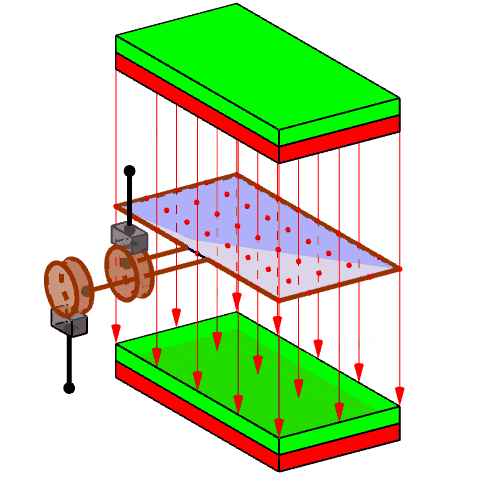
\includegraphics[width=3cm]{./Electric-generator-animation-5.png}};

            \node[
                above
            ]
            (B) 
            at (90,200)
            {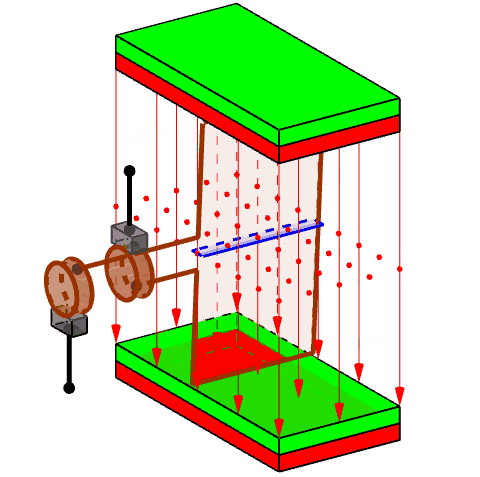
\includegraphics[width=3cm]{./Electric-generator-animation-17.png}};

            \node[
                above
            ]
            (C) 
            at (180,200)
            {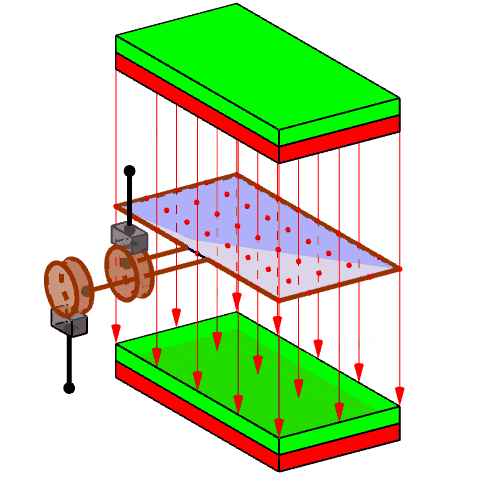
\includegraphics[width=3cm]{./Electric-generator-animation-5.png}};

            \node[
                above
            ]
            (D) 
            at (270,200)
            {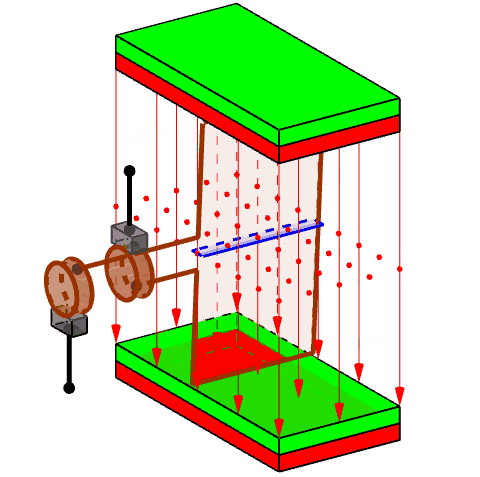
\includegraphics[width=3cm]{./Electric-generator-animation-17.png}};

            \node[
                above
            ]
            (E) 
            at (360,200)
            {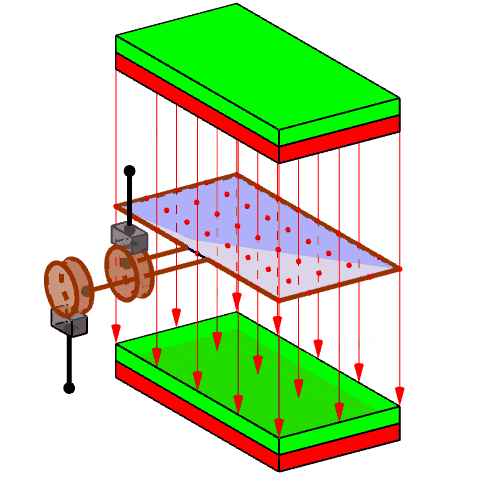
\includegraphics[width=3cm]{./Electric-generator-animation-5.png}};

            \draw[
                BakerADARed,
                dashed
            ]
            (B.south)
            -- (90,0)
            node[
                pos=0.75,
                right,
                text=BakerBlack
            ]
            {1/4 turn};

            \draw[
                BakerADARed,
                dashed
            ]
            (C.south)
            -- (180,0)
            node[
                pos=0.75,
                right,
                text=BakerBlack
            ]
            {1/2 turn};

            \draw[
                BakerADARed,
                dashed
            ]
            (D.south)
            -- (270,0)
            node[
                pos=0.75,
                right,
                text=BakerBlack
            ]
            {3/4 turn};

            \draw[
                BakerADARed,
                dashed
            ]
            (E.south)
            -- (360,0)
            node[
                pos=0.75,
                right,
                text=BakerBlack
            ]
            {1 turn};
            
            \draw[
                UpNorthGreen,
                dashed
            ]
            (180,0)
            -- (180,-60)
            coordinate[pos=0.75](alt);

            \draw[
                UpNorthGreen,
                <->
            ]
            (alt)
            -- (alt -| A.south)
            node[
                text=BakerBlack,
                pos=0.5,
                below
            ]{1 alternation};

            \draw[
                UpNorthGreen,
                dashed
            ]
            (360,0)
            -- (360,-230)
            coordinate[pos=0.875](cycle);

            \draw[
                UpNorthGreen,
                <->
            ]
            (cycle)
            -- (cycle -| A.south)
            node[
                text=BakerBlack,
                pos=0.5,
                below
            ]{1 cycle};
        
        \end{axis}

\end{circuitikz}
        }

        {\tiny \textbf{Attribution:} Adapted from \href{https://commons.wikimedia.org/wiki/File:Electric-generator-animation.gif}{``Electric Generator Animation''} (frames 5 and 17 extracted) by MikeRun, \href{https://creativecommons.org/licenses/by-sa/4.0}{CC BY-SA 4.0}, via Wikimedia Commons.\\[0.5em]}

        {\footnotesize The sine wave is caused by the physical layout of an AC generator -- as the coil spins inside the magnetic field it cuts the field in different directions, leading to a reverse in polarity\par}

    \end{figure}

\end{frame}

\begin{frame}
    \frametitle{AC Voltage - Alternation}

    \begin{figure}
        \centering
        \resizebox{0.48\linewidth}{!}{
            \begin{circuitikz}[
        american, 
        >={Latex[length=5mm, width=2mm]},
        %>=latex,
        alt={}
    ]

        \begin{axis}[
            width=6in,
            height=4in,
            axis lines=middle,
            color=BakerBlack,           % Sets default draw/text color for the axis
            axis line style={BakerBlack},
            tick style={BakerBlack},
            label style={BakerBlack},
            tick label style={BakerBlack},
            xlabel={Time ($t$)},        
            xlabel style={at={(ticklabel* cs:1)}, anchor=west},
            ylabel={Voltage ($V$)},
            ylabel near ticks,
            xmin=0, xmax=370,
            ymin=-200, ymax=200,
            xtick={0, 90, 180, 270, 360},
            xticklabels={$0^\circ$, $90^\circ$, $180^\circ$, $270^\circ$, $360^\circ$},
            ytick={-169.706, 0, 169.706},
            yticklabels={},
            grid=none,
            %grid style={dashed, gray!30},
            enlargelimits=false,
            clip=false
        ]
            % pgfplots trig functions expect degrees by default
            \addplot[domain=0:180, samples=100, ultra thick, LakeBlue] {169.706 * sin(x)};

            \addplot[domain=180:360, samples=100, ultra thick, BakerADARed] {169.706 * sin(x)};

            \node[
                above
            ]
            (A) 
            at (0,200)
            {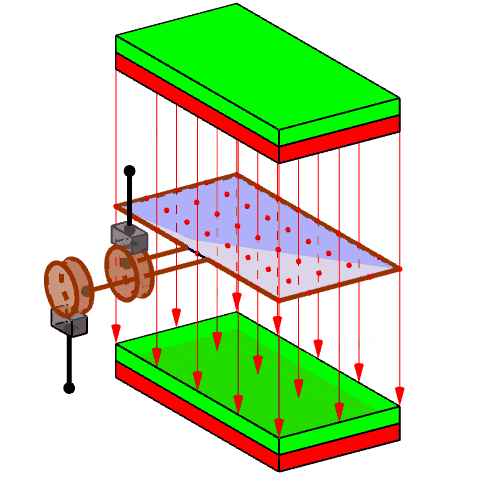
\includegraphics[width=3cm]{./Electric-generator-animation-5.png}};

            \node[
                above
            ]
            (B) 
            at (90,200)
            {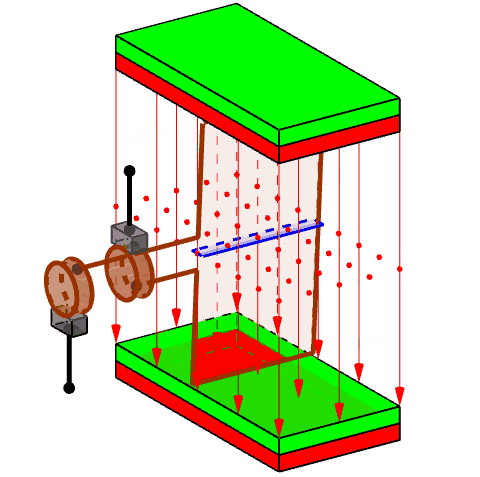
\includegraphics[width=3cm]{./Electric-generator-animation-17.png}};

            \node[
                above
            ]
            (C) 
            at (180,200)
            {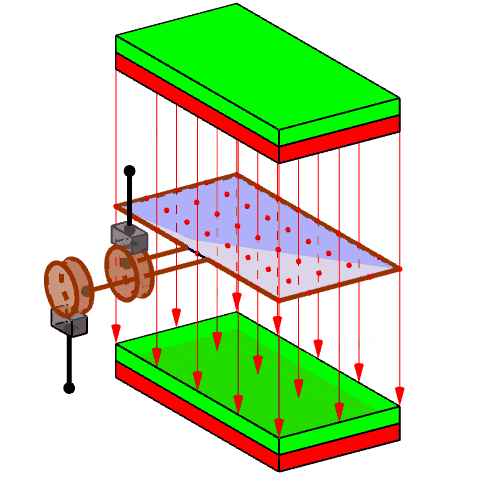
\includegraphics[width=3cm]{./Electric-generator-animation-5.png}};

            \node[
                above
            ]
            (D) 
            at (270,200)
            {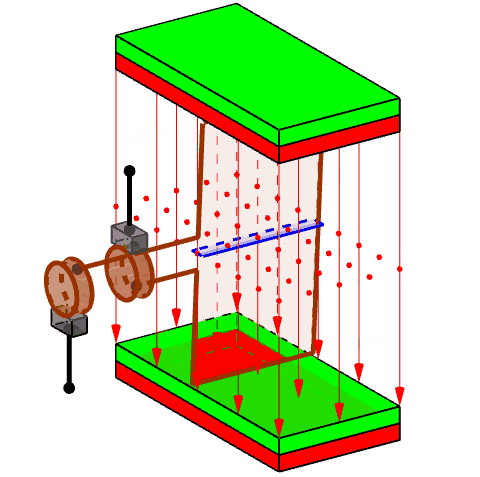
\includegraphics[width=3cm]{./Electric-generator-animation-17.png}};

            \node[
                above
            ]
            (E) 
            at (360,200)
            {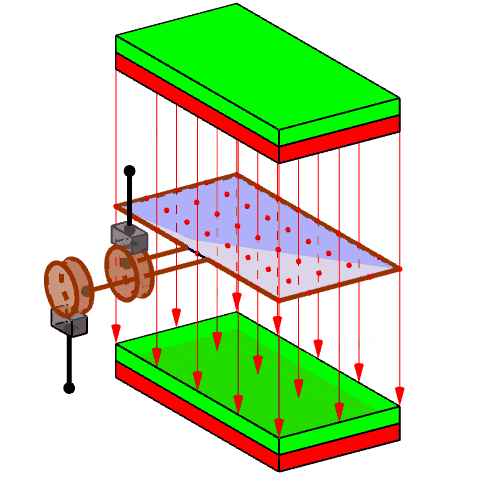
\includegraphics[width=3cm]{./Electric-generator-animation-5.png}};

            \draw[
                BakerADARed,
                dashed
            ]
            (B.south)
            -- (90,0)
            node[
                pos=0.75,
                right,
                text=BakerBlack
            ]
            {1/4 turn};

            \draw[
                BakerADARed,
                dashed
            ]
            (C.south)
            -- (180,0)
            node[
                pos=0.75,
                right,
                text=BakerBlack
            ]
            {1/2 turn};

            \draw[
                BakerADARed,
                dashed
            ]
            (D.south)
            -- (270,0)
            node[
                pos=0.75,
                right,
                text=BakerBlack
            ]
            {3/4 turn};

            \draw[
                BakerADARed,
                dashed
            ]
            (E.south)
            -- (360,0)
            node[
                pos=0.75,
                right,
                text=BakerBlack
            ]
            {1 turn};
            
            \draw[
                UpNorthGreen,
                dashed
            ]
            (180,0)
            -- (180,-60)
            coordinate[pos=0.75](alt);

            \draw[
                UpNorthGreen,
                <->
            ]
            (alt)
            -- (alt -| A.south)
            node[
                text=BakerBlack,
                pos=0.5,
                below
            ]{1 alternation};

            \draw[
                UpNorthGreen,
                dashed
            ]
            (360,0)
            -- (360,-230)
            coordinate[pos=0.875](cycle);

            \draw[
                UpNorthGreen,
                <->
            ]
            (cycle)
            -- (cycle -| A.south)
            node[
                text=BakerBlack,
                pos=0.5,
                below
            ]{1 cycle};
        
        \end{axis}

\end{circuitikz}
        }

        {\tiny \textbf{Attribution:} Adapted from \href{https://commons.wikimedia.org/wiki/File:Electric-generator-animation.gif}{``Electric Generator Animation''} (frames 5 and 17 extracted) by MikeRun, \href{https://creativecommons.org/licenses/by-sa/4.0}{CC BY-SA 4.0}, via Wikimedia Commons.\\[0.5em]}

        {\footnotesize An \emph{alternation} is 1/2 of a rotation of the coil--the point at which the polarity changes\par}

    \end{figure}

\end{frame}

\begin{frame}
    \frametitle{AC Voltage - Cycle}

    \begin{figure}
        \centering
        \resizebox{0.48\linewidth}{!}{
            \begin{circuitikz}[
        american, 
        >={Latex[length=5mm, width=2mm]},
        %>=latex,
        alt={}
    ]

        \begin{axis}[
            width=6in,
            height=4in,
            axis lines=middle,
            color=BakerBlack,           % Sets default draw/text color for the axis
            axis line style={BakerBlack},
            tick style={BakerBlack},
            label style={BakerBlack},
            tick label style={BakerBlack},
            xlabel={Time ($t$)},        
            xlabel style={at={(ticklabel* cs:1)}, anchor=west},
            ylabel={Voltage ($V$)},
            ylabel near ticks,
            xmin=0, xmax=370,
            ymin=-200, ymax=200,
            xtick={0, 90, 180, 270, 360},
            xticklabels={$0^\circ$, $90^\circ$, $180^\circ$, $270^\circ$, $360^\circ$},
            ytick={-169.706, 0, 169.706},
            yticklabels={},
            grid=none,
            %grid style={dashed, gray!30},
            enlargelimits=false,
            clip=false
        ]
            % pgfplots trig functions expect degrees by default
            \addplot[domain=0:180, samples=100, ultra thick, LakeBlue] {169.706 * sin(x)};

            \addplot[domain=180:360, samples=100, ultra thick, BakerADARed] {169.706 * sin(x)};

            \node[
                above
            ]
            (A) 
            at (0,200)
            {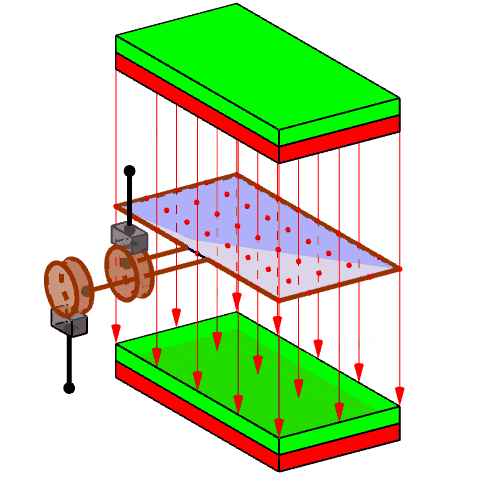
\includegraphics[width=3cm]{./Electric-generator-animation-5.png}};

            \node[
                above
            ]
            (B) 
            at (90,200)
            {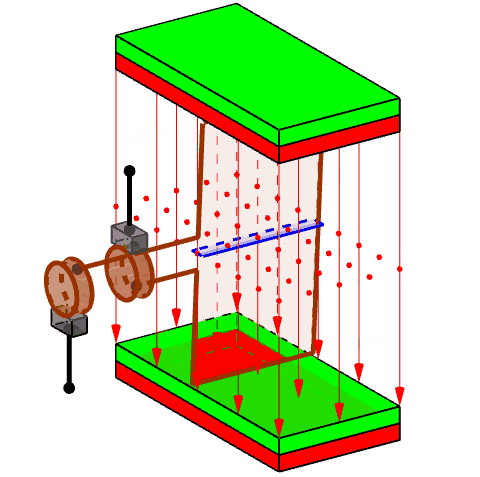
\includegraphics[width=3cm]{./Electric-generator-animation-17.png}};

            \node[
                above
            ]
            (C) 
            at (180,200)
            {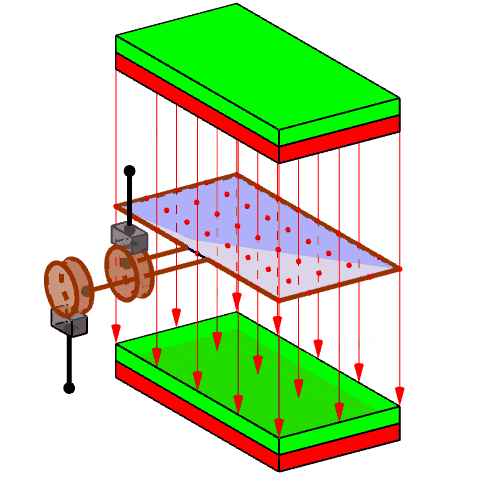
\includegraphics[width=3cm]{./Electric-generator-animation-5.png}};

            \node[
                above
            ]
            (D) 
            at (270,200)
            {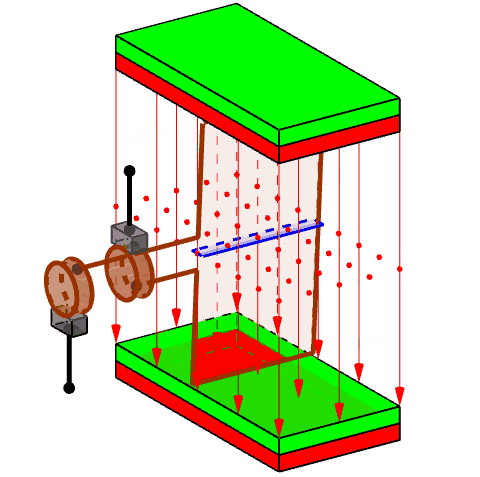
\includegraphics[width=3cm]{./Electric-generator-animation-17.png}};

            \node[
                above
            ]
            (E) 
            at (360,200)
            {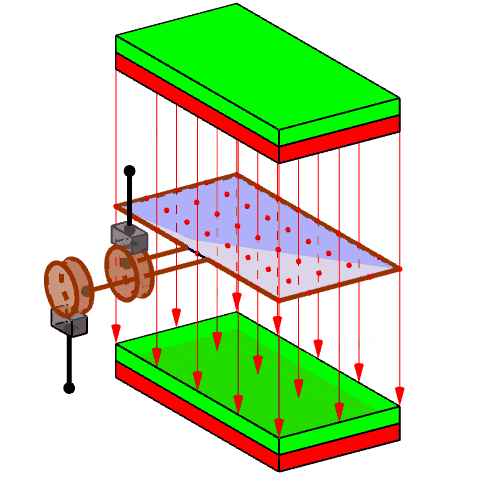
\includegraphics[width=3cm]{./Electric-generator-animation-5.png}};

            \draw[
                BakerADARed,
                dashed
            ]
            (B.south)
            -- (90,0)
            node[
                pos=0.75,
                right,
                text=BakerBlack
            ]
            {1/4 turn};

            \draw[
                BakerADARed,
                dashed
            ]
            (C.south)
            -- (180,0)
            node[
                pos=0.75,
                right,
                text=BakerBlack
            ]
            {1/2 turn};

            \draw[
                BakerADARed,
                dashed
            ]
            (D.south)
            -- (270,0)
            node[
                pos=0.75,
                right,
                text=BakerBlack
            ]
            {3/4 turn};

            \draw[
                BakerADARed,
                dashed
            ]
            (E.south)
            -- (360,0)
            node[
                pos=0.75,
                right,
                text=BakerBlack
            ]
            {1 turn};
            
            \draw[
                UpNorthGreen,
                dashed
            ]
            (180,0)
            -- (180,-60)
            coordinate[pos=0.75](alt);

            \draw[
                UpNorthGreen,
                <->
            ]
            (alt)
            -- (alt -| A.south)
            node[
                text=BakerBlack,
                pos=0.5,
                below
            ]{1 alternation};

            \draw[
                UpNorthGreen,
                dashed
            ]
            (360,0)
            -- (360,-230)
            coordinate[pos=0.875](cycle);

            \draw[
                UpNorthGreen,
                <->
            ]
            (cycle)
            -- (cycle -| A.south)
            node[
                text=BakerBlack,
                pos=0.5,
                below
            ]{1 cycle};
        
        \end{axis}

\end{circuitikz}
        }

        {\tiny \textbf{Attribution:} Adapted from \href{https://commons.wikimedia.org/wiki/File:Electric-generator-animation.gif}{``Electric Generator Animation''} (frames 5 and 17 extracted) by MikeRun, \href{https://creativecommons.org/licenses/by-sa/4.0}{CC BY-SA 4.0}, via Wikimedia Commons.\\[0.5em]}

        {\footnotesize A \emph{cycle} is a full rotation of the coil\par}

    \end{figure}

\end{frame}

\begin{frame}
    \frametitle{AC Voltage - Frequency}

    \begin{figure}
        \centering
        \resizebox{0.75\linewidth}{!}{
            \begin{circuitikz}[
    american,
    >=latex,
    alt={}
]

    \begin{axis}[
        width=6in,
        height=4in,
        axis lines=middle,
        x axis line style={-},
        y axis line style={-},  
        color=BakerBlack,           % Sets default draw/text color for the axis
        axis line style={BakerBlack},
        tick style={BakerBlack},
        label style={BakerBlack},
        tick label style={BakerBlack},
        scaled x ticks=false,
        xlabel={{Time (s)}},
        xlabel style={at={(ticklabel* cs:1)}, anchor=west},
        ylabel={{Voltage (V)}},
        ylabel near ticks,
        xmin=0, xmax=370,
        ymin=-200, ymax=200,
        xtick={0, 90, 180, 270, 360},
        xticklabels={0, {1/240}, {1/120}, {1/80}, {1/60}},
        ytick={-169.706, 0, 169.706},
        yticklabels={},
        grid=none,
        %grid style={dashed, gray!30},
        enlargelimits=false,
        clip=false
    ]
        % pgfplots trig functions expect degrees by default
        \addplot[domain=0:360, samples=200, ultra thick, LakeBlue] {169.706 * sin(x)};

    \end{axis}

\end{circuitikz}
        }

        {\footnotesize The frequency is the number of cycles per second (Hz)--the U.S. standard is 60 Hz (60 cycles per second)\par}

    \end{figure}

\end{frame}

\begin{frame}
    \frametitle{Visualizing Frequency}
    \begin{columns}
        \begin{column}{0.48\linewidth}
            \begin{figure}
                \centering
                \resizebox{\columnwidth}{!}{
                    \begin{circuitikz}[
    american,
    >=latex,
    alt={}
]

    \begin{axis}[
        width=6in,
        height=4in,
        axis lines=middle,
        x axis line style={-},
        y axis line style={-},  
        color=BakerBlack,           % Sets default draw/text color for the axis
        axis line style={BakerBlack},
        tick style={BakerBlack},
        label style={BakerBlack},
        tick label style={BakerBlack},
        scaled x ticks=false,
        xlabel={{Time (s)}},
        xlabel style={at={(ticklabel* cs:1)}, anchor=west},
        ylabel={{Voltage (V)}},
        ylabel near ticks,
        xmin=0, xmax=370,
        ymin=-200, ymax=200,
        xtick={0, 90, 180, 270, 360},
        xticklabels={0, {1/240}, {1/120}, {1/80}, {1/60}},
        ytick={-169.706, 0, 169.706},
        yticklabels={},
        grid=none,
        %grid style={dashed, gray!30},
        enlargelimits=false,
        clip=false
    ]
        % pgfplots trig functions expect degrees by default
        \addplot[domain=0:360, samples=200, ultra thick, LakeBlue] {169.706 * sin(x)};

    \end{axis}

\end{circuitikz}
                }
            \end{figure}
        \end{column}
        \begin{column}{0.48\linewidth}
            \begin{figure}
                \centering
                \resizebox{\columnwidth}{!}{
                    \begin{circuitikz}[
    american,
    >=latex,
    alt={}
]

    \begin{axis}[
        width=6in,
        height=4in,
        axis lines=middle,
        x axis line style={-},
        y axis line style={-},  
        color=BakerBlack,           % Sets default draw/text color for the axis
        axis line style={BakerBlack},
        tick style={BakerBlack},
        label style={BakerBlack},
        tick label style={BakerBlack},
        scaled x ticks=false,
        xlabel={{Time (s)}},
        xlabel style={at={(ticklabel* cs:1)}, anchor=west},
        ylabel={{Voltage (V)}},
        ylabel near ticks,
        xmin=0, xmax=22500,
        ymin=-200, ymax=200,
        xtick={0, 5400, 10800, 16200, 21600},
        xticklabels={0, {1/4}, {1/2}, {3/4}, 1},
        ytick={-169.706, 0, 169.706},
        yticklabels={},
        grid=none,
        %grid style={dashed, gray!30},
        enlargelimits=false,
        clip=false
    ]
        % pgfplots trig functions expect degrees by default
        \addplot[domain=0:21600, samples=6000, ultra thick, LakeBlue] {169.706 * sin(x)};

    \end{axis}

\end{circuitikz}
                }
            \end{figure}
        \end{column}
    \end{columns}
    \centering
    {\footnotesize We often use one cycle (left) to visualize the curve, but remember that that one cycle is happening 60 times every second (right)\par}
\end{frame}

% \begin{frame}
%     \frametitle{AC Voltage - Phases}
%     \begin{columns}
%         \begin{column}{0.48\linewidth}
%             \begin{figure}
%                 \centering
%                 \resizebox{\columnwidth}{!}{
%                     \begin{circuitikz}[
    american,
    >=latex,
    alt={}
]

    \begin{axis}[
        name=SinglePhasePlot,
        width=6in,
        height=4in,
        axis lines=middle,
        color=BakerBlack,           % Sets default draw/text color for the axis
        axis line style={BakerBlack},
        tick style={BakerBlack},
        label style={BakerBlack},
        tick label style={BakerBlack},
        xlabel={Time ($t$)},        
        xlabel style={at={(ticklabel* cs:1)}, anchor=west},
        ylabel={Voltage ($V$)},
        ylabel near ticks,
        xmin=0, xmax=370,
        ymin=-200, ymax=200,
        xtick={0, 90, 180, 270, 360},
        xticklabels={$0^\circ$, $90^\circ$, $180^\circ$, $270^\circ$, $360^\circ$},
        ytick={-169.706, 0, 169.706},
        yticklabels={},
        grid=none,
        %grid style={dashed, gray!30},
        enlargelimits=false,
        clip=false
    ]
        % pgfplots trig functions expect degrees by default
        \addplot[domain=0:360, samples=200, ultra thick, LakeBlue] {169.706 * sin(x)};

    \end{axis}

    


\end{circuitikz}
%                 }
%             \end{figure}
%         \end{column}
%         \begin{column}{0.48\linewidth}
%             \begin{figure}
%                 \centering
%                 \resizebox{\columnwidth}{!}{
%                     \begin{circuitikz}[
    american,
    >=latex,
    alt={}
]

    \begin{axis}[
        width=6in,
        height=4in,
        axis lines=middle,
        x axis line style={-},
        y axis line style={-},  
        color=BakerBlack,           % Sets default draw/text color for the axis
        axis line style={BakerBlack},
        tick style={BakerBlack},
        label style={BakerBlack},
        tick label style={BakerBlack},
        xlabel={Time ($t$)},        
        xlabel style={at={(ticklabel* cs:1)}, anchor=west},
        ylabel={Voltage ($V$)},
        ylabel near ticks,
        xmin=0, xmax=370,
        ymin=-500, ymax=500,
        xtick={0, 90, 180, 270, 360},
        xticklabels={$0^\circ$, $90^\circ$, $180^\circ$, $270^\circ$, $360^\circ$},
        ytick={-480, 0, 480},
        yticklabels={},
        grid=none,
        %grid style={dashed, gray!30},
        enlargelimits=false,
        clip=false
    ]
        % pgfplots trig functions expect degrees by default
        \addplot[domain=0:360, samples=200, ultra thick, BakerBlack] {480 * sin(x)};

        \addplot[domain=0:360, samples=200, ultra thick, HoneyYellow] {480 * sin(x - 120)};

        \addplot[domain=0:360, samples=200, ultra thick, BakerADARed] {480 * sin(x + 120)};
    
        \node[
            text=BakerBlack,
            above
        ]
        at (90,480)
        {A};

        \node[
            text=HoneyYellow,
            above
        ]
        at (210,480)
        {B};

        \node[
            text=BakerADARed,
            above
        ]
        at (330,480)
        {C};

    \end{axis}

\end{circuitikz}
%                 }
%             \end{figure}
%         \end{column}
%     \end{columns}
% \end{frame}

\subsection{Converting AC to DC}

\begin{frame}
    \frametitle{Bridge Rectifier}

    \begin{figure}
        \centering
        \resizebox{0.48\linewidth}{!}{
            \begin{circuitikz}[
        american, 
        %>={Latex[length=5mm, width=2mm]},
        >=latex,
        alt={}
    ]

    \draw[
        BakerBlack
    ]
    (0,0)
    coordinate(sTop)
    -- ++(2,0)
    coordinate(left)
    to[D*, color=BakerBlack, *-*] ++(3,3)
    coordinate(top)
    -- ++(6,0)
    node[
        right,
        circle,
        draw=BakerBlack,
        minimum size=0.125cm
    ](outTop){};

    \draw[
        BakerBlack
    ]
    (0,-4)
    coordinate(sBottom)
    -- ++(9,0)
    -- ++(0,4)
    -- ++(-1,0)
    coordinate(right)
    to[D*, color=BakerBlack, *-*] ++(-3,3);

    \node[
        draw=BakerBlack,
        circle,
        minimum size=0.125cm
    ](outBottom)
    at ($(outTop)-(0,6)$)
    {};

    \draw[
        BakerBlack
    ]
    (outBottom.west)
    -- ++(-6,0)
    coordinate(bottom)
    to[D*, color=BakerBlack, *-*] ++(3,3);

    \draw[
        BakerBlack
    ]
    (bottom)
    to[D*, color=BakerBlack] (left);

    \draw[
        BakerBlack
    ]
    (sBottom)
    to[sV, color=BakerBlack] (sTop);

\end{circuitikz}
        }

        {\footnotesize A \emph{bridge rectifier} is commonly used in controls applications to convert AC to DC}

    \end{figure}

\end{frame}

\begin{frame}
    \frametitle{Bridge Rectifier - Active}

    \begin{columns}
        \begin{column}{0.48\linewidth}
            \begin{figure}
                \centering
                \resizebox{0.9\columnwidth}{!}{
                    \begin{circuitikz}[
        american, 
        %>={Latex[length=5mm, width=2mm]},
        >=latex,
        alt={}
    ]

    % Coordinates for the bridge
    \coordinate (psBottom) at (0,-1);
    \coordinate (psTop) at (0,3);
    \coordinate (left) at (2,3);
    \coordinate (top) at (4.5,5.5);
    \coordinate (right) at (7,3);
    \coordinate (bottom) at (4.5,0.5);
    \coordinate (rB) at (8,-1);
    \coordinate (rT) at (8,3);
    \coordinate (plus) at (10,5.5);
    \coordinate (minus) at (10,0.5);

    % Colored components on main layer, black items will go below on the bg layer
    \begin{pgfonlayer}{main}

        % Power supply
        \draw[
            LakeBlue
        ]
        (psBottom)
        to[sV, color=LakeBlue, l=V] (psTop);

        % Output nodes
        \node[
            draw=LakeBlue,
            text=LakeBlue,
            circle,
            minimum size=0.25,
            label={right:+}
        ]
        (pOut)
        at (plus)
        {};

        \node[
            draw=BakerADARed,
            text=BakerADARed,
            circle,
            minimum size=0.25,
            label={right:{--}}
        ]
        (mOut)
        at (minus)
        {};

        % Draw from power supply top, upper left diode, positive output
        \draw[
            LakeBlue
        ]
        (psTop)
        -- (left)
        to[D*, color=LakeBlue, *-*] (top)
        -- (pOut.west);

        % Draw back from minus output, lower right diode, back to power supply bottom
        \draw[
            BakerADARed
        ]
        (mOut.west)
        -- (bottom)
        to[D*, color=BakerADARed, *-*] (right)
        -- (rT)
        -- (rB)
        -- (psBottom);        
    
    \end{pgfonlayer}

    \begin{pgfonlayer}{bg}
        
        % Upper right diode
        \draw[
            BakerBlack
        ]
        (right)
        to[D*, color=BakerBlack] (top);

        \draw[
            BakerBlack
        ]
        (bottom)
        to[D*, color=BakerBlack] (left);

    \end{pgfonlayer}    

\end{circuitikz}
                }

                {\tiny Positive AC Cycle\par}
            \end{figure}
        \end{column}
        \begin{column}{0.48\linewidth}
            \begin{figure}
                \centering
                \resizebox{\columnwidth}{!}{
                    \begin{circuitikz}[
        american, 
        %>={Latex[length=5mm, width=2mm]},
        >=latex,
        alt={Circuit schematic of a full wave bridge rectifier highlighting the conduction path during the negative half cycle of the AC input voltage. The active current path from the bottom of the AC source, through diode D3 at the top right, to the positive output node labeled with a plus sign is highlighted in blue. The return path from the negative output node labeled with a minus sign, through diode D4 at the bottom left, to the top of the AC source is highlighted in red. Diodes D1 and D2 remain inactive and are drawn in black.}
    ]

    % Coordinates for the bridge
    \coordinate (psBottom) at (0,-1);
    \coordinate (psTop) at (0,3);
    \coordinate (left) at (2,3);
    \coordinate (top) at (4.5,5.5);
    \coordinate (right) at (7,3);
    \coordinate (bottom) at (4.5,0.5);
    \coordinate (rB) at (8,-1);
    \coordinate (rT) at (8,3);
    \coordinate (plus) at (10,5.5);
    \coordinate (minus) at (10,0.5);

    % Colored components on main layer, black items will go below on the bg layer
    \begin{pgfonlayer}{main}

        % Output nodes
        \node[
            draw=LakeBlue,
            text=LakeBlue,
            font=\bfseries,
            circle,
            minimum size=0.25,
            label={[LakeBlue]right:+}
        ]
        (pOut)
        at (plus)
        {};

        \node[
            draw=BakerADARed,
            text=BakerADARed,
            font=\bfseries,
            circle,
            minimum size=0.25,
            label={[BakerADARed]right:{--}}
        ]
        (mOut)
        at (minus)
        {};

        \draw[
            LakeBlue
        ]
        (psBottom)
        -- (rB)
        -- (rT)
        -- (right)
        to[D*=$D_3$, color=LakeBlue, *-*] (top)
        -- (pOut.west);

        \draw[
            BakerADARed
        ]
        (mOut.west)
        -- (bottom)
        to[D*=$D_4$, color=BakerADARed, *-*] (left)
        -- (psTop);

        \draw[
            LakeBlue
        ]
        (psBottom)
        -- ++(0,1.5)
        coordinate(sVbottom);

        \draw[
            BakerADARed
        ]
        (sVbottom)
        to[sV=$V$, color=BakerADARed] ++(0,1)
        -- (psTop);
    
    \end{pgfonlayer}

    \begin{pgfonlayer}{bg}
        
        \draw[
            BakerBlack
        ]
        (left)
        to[D*=$D_1$, color=BakerBlack] (top);

        \draw[
            BakerBlack
        ]
        (bottom)
        to[D*=$D_2$, color=BakerBlack] (right);

    \end{pgfonlayer}    

\end{circuitikz}
                }
                
                {\tiny Negative AC Cycle\par}
            \end{figure}
        \end{column}
    \end{columns}

    \vspace{0.5em}
    \centering
    {\footnotesize As the polarity of the AC voltages changes the the rectifier forces the output to the same polarity\par}

\end{frame}

\begin{frame}
    \frametitle{Rectified Alternating Current}

    \begin{figure}
        \centering
        \resizebox{0.75\linewidth}{!}{
            \begin{circuitikz}[
    american,
    %>=latex,
    >={Latex[length=3mm, width=1.5mm]},
    alt={Line graph showing full wave rectification of a 120 volt RMS AC sine wave over three full cycles, plotted with voltage on the vertical axis against time on the horizontal axis. A dashed blue curve represents the input alternating current voltage oscillating smoothly between positive 169.7 volts and negative 169.7 volts. Overlaid on top is a solid red curve representing the output rectified voltage, where the positive half-cycles follow the blue sine wave and the negative half-cycles are inverted upwards into positive pulses, resulting in continuous positive voltage peaks. A label points to a negative trough of the input sine wave as Vin, and another label points to an inverted positive crest of the rectified wave as Vout.}
]

    \begin{axis}[
        name=SinglePhasePlot,
        width=6in,
        height=4in,
        axis lines=middle,
        color=BakerBlack,           % Sets default draw/text color for the axis
        axis line style={BakerBlack},
        tick style={BakerBlack},
        label style={BakerBlack},
        tick label style={BakerBlack},
        xlabel={Time ($t$)},        
        xlabel style={at={(ticklabel* cs:1)}, anchor=west},
        ylabel={Voltage ($V$)},
        ylabel near ticks,
        xmin=0, xmax=1100,
        ymin=-200, ymax=200,
        xtick={},
        xticklabels={},
        ytick={},
        yticklabels={},
        grid=none,
        %grid style={dashed, gray!30},
        enlargelimits=false,
        clip=false
    ]
        % pgfplots trig functions expect degrees by default
        \addplot[domain=0:1080, samples=600, line width=2.5pt, dashed, LakeBlue] {169.706 * sin(x)};

        \addplot[domain=0:1080, samples=600, ultra thin, BakerADARed] {169.706 * sin(x) > 0 ? 169.706 * sin(x) : -169.706 * sin(x)};

        \draw[
            UpNorthGreen,
            <-
        ]
        (270,-170)
        to[out=300, in=180] (320,-190)
        node[
            text=BakerBlack,
            anchor=west
        ]{$V_{\text{in}}$};

        \draw[
            UpNorthGreen,
            <-
        ]
        (270,170)
        to[out=60, in=180] (320,190)
        node[
            text=BakerBlack,
            anchor=west
        ]{$V_{\text{out}}$};

    \end{axis}

    


\end{circuitikz}
        }

        {\footnotesize The rectifier redirects current so the output is always the same polarity, but it \emph{does not} affect the voltage value--the resulting wave is DC, but not very useful DC\par}

    \end{figure}

\end{frame}

\begin{frame}
    \frametitle{Bridge Rectifier - Smoothed}

    \begin{figure}
        \centering
        \resizebox{0.75\linewidth}{!}{
            \begin{circuitikz}[
        american, 
        %>={Latex[length=5mm, width=2mm]},
        >=latex,
        alt={Circuit schematic of a full wave bridge rectifier circuit with a filter capacitor. An alternating current sinusoidal voltage source is connected to the input terminals of a diamond-shaped diode bridge consisting of four diodes labeled D1, D2, D3, and D4. The top output node of the diode bridge connects to a positive output terminal marked with a plus sign, while the bottom output node connects to a negative output terminal marked with a minus sign. Connected in parallel across the positive and negative output DC rails between the diode bridge and the output terminals is a capacitor, which serves to filter and smooth the rectified direct current voltage delivered to the load.}
    ]

    % Coordinates for the bridge
    \coordinate (psBottom) at (0,-1);
    \coordinate (psTop) at (0,3);
    \coordinate (left) at (2,3);
    \coordinate (top) at (4.5,5.5);
    \coordinate (right) at (7,3);
    \coordinate (bottom) at (4.5,0.5);
    \coordinate (rB) at (8,-1);
    \coordinate (rT) at (8,3);
    \coordinate (plus) at (10,5.5);
    \coordinate (minus) at (10,0.5);

    % Colored components on main layer, black items will go below on the bg layer
    \begin{pgfonlayer}{main}

        % Power supply
        \draw[
            BakerBlack
        ]
        (psBottom)
        to[sV, color=BakerBlack] (psTop);

        % Output nodes
        \node[
            draw=BakerBlack,
            text=BakerBlack,
            circle,
            minimum size=0.25,
            label={right:+}
        ]
        (pOut)
        at ($(plus)+(2,0)$)
        {};

        \node[
            draw=BakerBlack,
            text=BakerBlack,
            circle,
            minimum size=0.25,
            label={right:{--}}
        ]
        (mOut)
        at ($(minus)+(2,0)$)
        {};

        \draw[
            BakerBlack
        ]
        (plus)
        to[C, color=BakerBlack] (minus);

        % Draw back from minus output, through lower left diode, to power supply top
        \draw[
            BakerBlack
        ]
        (mOut.west)
        to[short,-*] (bottom)
        to[D*=$D_4$, color=BakerBlack, -*] (left)
        -- (psTop);

        % Draw from power supply bottom, through upper right diode, to positive output
        \draw[
            BakerBlack
        ]
        (psBottom)
        -- (rB)
        -- (rT)
        -- (right)
        to[D*=$D_3$, color=BakerBlack, *-*] (top)
        -- (pOut.west);
    
    \end{pgfonlayer}

    \begin{pgfonlayer}{bg}
        
        % Upper left diode
        \draw[
            BakerBlack
        ]
        (left)
        to[D*=$D_1$, color=BakerBlack] (top);

        % Lower right diode
        \draw[
            BakerBlack
        ]
        (bottom)
        to[D*=$D_2$, color=BakerBlack] (right);

    \end{pgfonlayer}    

\end{circuitikz}
        }

        {\footnotesize Smoothing capacitors are added to help maintain the voltage level between cycles, which helps keep the DC at a more consistent value\par}

    \end{figure}

\end{frame}

\begin{frame}
    \frametitle{Rectified and Smoothed Alternating Current}

    \begin{figure}
        \centering
        \resizebox{0.75\linewidth}{!}{
            \begin{circuitikz}[
    american,
    >=latex,
    alt={Line graph showing full wave rectification with capacitor smoothing over three cycles, plotted with voltage on the vertical axis against time on the horizontal axis. A dashed blue curve shows the input alternating current voltage oscillating between positive 169.7 volts and negative 169.7 volts. A fine black dotted curve outlines the underlying full wave rectified positive pulses. Overlaid on top is a solid red output voltage curve demonstrating the smoothing effect of a filter capacitor. On startup, the red curve rises from zero volts along the initial sine wave to the first peak of 169.7 volts. From there, it gradually decays downward exponentially as the capacitor discharges, before intercepting the rising edge of the next rectified peak and charging back up to maximum voltage. This cycle repeats continuously across subsequent peaks, creating a smoothed direct current output with a slight voltage ripple near maximum amplitude.}
]

    \begin{axis}[
        name=SinglePhasePlot,
        width=6in,
        height=4in,
        axis lines=middle,
        color=BakerBlack,           % Sets default draw/text color for the axis
        axis line style={BakerBlack},
        tick style={BakerBlack},
        label style={BakerBlack},
        tick label style={BakerBlack},
        xlabel={Time ($t$)},        
        xlabel style={at={(ticklabel* cs:1)}, anchor=west},
        ylabel={Voltage ($V$)},
        ylabel near ticks,
        xmin=0, xmax=1100,
        ymin=-200, ymax=200,
        xtick={},
        xticklabels={},
        ytick={},
        yticklabels={},
        grid=none,
        %grid style={dashed, gray!30},
        enlargelimits=false,
        clip=false
    ]
        % pgfplots trig functions expect degrees by default
        \addplot[domain=0:1080, samples=600, line width=2.5pt, dashed, LakeBlue] {169.706 * sin(x)};

        \addplot[domain=0:1080, samples=600, thin, dotted, BakerBlack] {169.706 * sin(x) > 0 ? 169.706 * sin(x) : -169.706 * sin(x)};

        \addplot[BakerADARed, ultra thin, domain=0:1080,samples=600] {
            169.706 * max(
                abs(sin(x)), 
                (x < 90 ? 0 : exp(-0.001 * mod(x - 90, 180)))
            )
        };

    \end{axis}

\end{circuitikz}
        }

        {\footnotesize The result is a fairly smooth DC wave--the \emph{ripple} will always be there, but can be tweaked by changing the capacitor value\par}
    \end{figure}

\end{frame}

\subsection{Resistance}

\begin{frame}
    \frametitle{Resistance Defined}

    \begin{figure}
        \centering
        \resizebox{0.75\linewidth}{!}{
            \begin{circuitikz}[
    american,
    %>=latex,
    >={Latex[length=3mm, width=1.5mm]},
    alt={Diagram showing a fluid flow or particle trajectory diagram illustrating laminar flow convergence or stream contraction through a narrowed channel throat. Three parallel blue directional arrows flow from left to right, with the outer top and bottom paths tapering inward to match a central constriction in the outer black boundary walls before continuing parallel on the right.}
]

    \draw[
        BakerBlack,
        rounded corners=0.5cm,
        line width=2.5pt
    ]
    (0,0)
    -- ++(4,0)
    -- ++(2,-1)
    -- ++(4,0);

    \draw[
        BakerBlack,
        rounded corners=0.5cm,
        line width=2.5pt
    ]
    (0,-3)
    -- ++(4,0)
    -- ++(2,1)
    -- ++(4,0);

    \draw[
        LakeBlue,
        ultra thick,
        rounded corners=0.375cm,
        ->
    ]
    (0,-0.5)
    -- ++(4,0)
    -- ++(2,-0.75)
    -- ++(4,0);

    \draw[
        LakeBlue,
        ultra thick,
        rounded corners=0.375cm,
        ->
    ]
    (0,-1.5)
    -- ++(10,0);

    \draw[
        LakeBlue,
        ultra thick,
        rounded corners=0.375cm,
        ->
    ]
    (0,-2.5)
    -- ++(4,0)
    -- ++(2,0.75)
    -- ++(4,0);

\end{circuitikz}
        }
    \end{figure}

    \vspace{0.5em}
    \centering
    {\footnotesize \emph{Resistance} is the opposition to electron flow--like a restriction in a water pipe\par}

\end{frame}

\begin{frame}
    \frametitle{Resistance Causes Heat}

    \begin{columns}
        \begin{column}{0.48\linewidth}
            \begin{itemize}
                \item{\emph{ALL} components in a circuit have resistance--including wires}
                \item{Current through a resistance \emph{always} comes with heat}
                \item{Unless we're actually building a heater, this is \emph{dissipated} (lost) energy}
            \end{itemize}            
        \end{column}
        \begin{column}{0.48\linewidth}
            \begin{figure}
                \centering

                %\hexpic[]{\columnwidth}{A cartridge heater being heated to a red hot state.}{../../assets/images/Cartridge-heater-hot.jpg}
                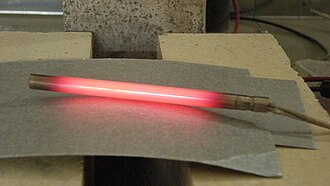
\includegraphics[width=0.9\columnwidth, alt={A cartridge heater being heated to a red hot state.}]{../../assets/images/Cartridge-heater-hot.jpg}

                {\tiny \textbf{Attribution:} Maxellator, \href{https://creativecommons.org/licenses/by-sa/3.0}{CC BY-SA 3.0}, via \href{https://commons.wikimedia.org/wiki/File:Cartridge-heater-hot.jpg}{Wikimedia Commons}\par}
            \end{figure}
        \end{column}
    \end{columns}    

\end{frame}

\begin{frame}
    \frametitle{Ohm's Law}

    \begin{figure}
        \centering
        \resizebox{0.375\linewidth}{!}{
            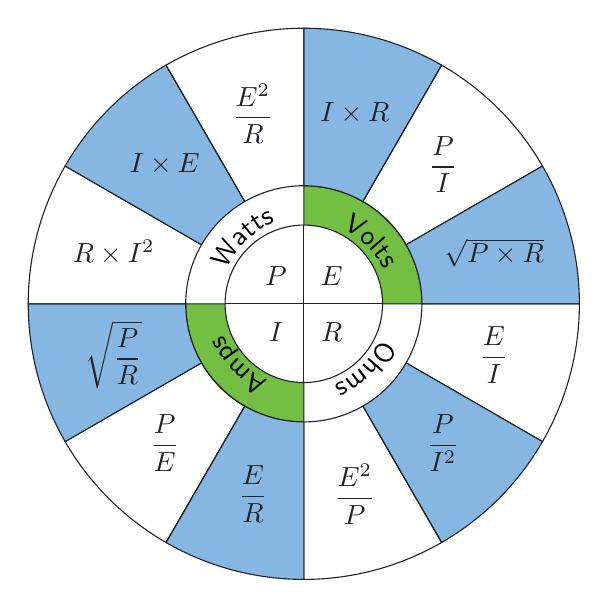
\begin{tikzpicture}

    %Volts
    \draw[BakerBlack, fill=UpNorthGreen] (0,1) arc (90:0:1cm) -- ++(0.5,0) arc (0:90:1.5cm) -- ++(0,-0.5);
    \draw[BakerBlack, fill=LakeBlue] (0,1.5) -- (0,3.5) arc (90:60:3.5cm) -- ++(240:2cm) arc (60:90:1.5cm);
    \draw[BakerBlack] (60:1.5cm) -- (60:3.5cm) arc (60:30:3.5cm) -- (30:1.5cm) arc (30:60:1.5cm);
    \draw[BakerBlack, fill=LakeBlue] (1.5,0) arc (0:30:1.5cm) -- (30:3.5cm) arc (30:0:3.5cm) -- (1.5,0);
    \draw[BakerBlack] (0,0) -- (0,1);
    \draw[BakerBlack] (0,0) -- (1,0);
    \node[text=BakerBlack, anchor=center, align=center] at (45:0.5cm){$E$};
    \node[text=BakerBlack, anchor=center, align=center] at (15:2.5cm){$\sqrt{P \times R}$};
    \node[text=BakerBlack, anchor=center, align=center] at (45:2.5cm){$\dfrac{P}{I}$};
    \node[text=BakerBlack, anchor=center, align=center] at (75:2.5cm){$I \times R$};
    \path[postaction={decorate},decoration={text along path, text={Volts},text align=center}] (0,1.0625) arc (90:0:1.125cm);

    %Ohms
    \draw[BakerBlack] (1.5,0) -- (3.5,0) arc (360:330:3.5cm) -- (330:1.5) arc (330:360:1.5);
    \draw[BakerBlack, fill=LakeBlue] (330:1.5) -- (330:3.5) arc (330:300:3.5) -- (300:1.5) arc (300:330:1.5);
    \draw[BakerBlack] (300:1.5) arc (300:270:1.5) -- (270:3.5) arc (270:300:3.5) -- (300:1.5);
    \draw[BakerBlack] (1,0) arc (360:270:1cm);
    \draw[BakerBlack] (0,0) -- (0,-1);
    \draw[BakerBlack] (0,-1) -- (0,-1.5);
    \node[text=BakerBlack, anchor=center, align=center] at (315:0.5cm){$R$};
    \node[text=BakerBlack, anchor=center, align=center] at (345:2.5cm){$\dfrac{E}{I}$};
    \node[text=BakerBlack, anchor=center, align=center] at (315:2.5cm){$\dfrac{P}{I^2}$};
    \node[text=BakerBlack, anchor=center, align=center] at (285:2.5cm){$\dfrac{E^2}{P}$};
    \path[postaction={decorate},decoration={text along path, text={Ohms},text align=center}] (1.0625,0) arc (360:270:1.125cm);

    %Amps
    \draw[BakerBlack, fill=UpNorthGreen] (0,-1) arc (270:180:1) -- (180:1.5) arc (180:270:1.5) -- (0,-1);
    \draw[BakerBlack, fill=LakeBlue] (270:1.5) -- (270:3.5) arc (270:240:3.5) -- (240:1.5) arc (240:270:1.5);
    \draw[BakerBlack] (240:1.5) -- (240:3.5) arc (240:210:3.5) -- (210:1.5) arc (210:240:1.5);
    \draw[BakerBlack, fill=LakeBlue] (210:1.5) -- (210:3.5) arc (210:180:3.5) -- (180:1.5) arc (180:210:1.5);
    \draw[BakerBlack] (0,0) -- (-1,0);
    \node[text=BakerBlack, anchor=center, align=center] at (225:0.5cm){$I$};
    \node[text=BakerBlack, anchor=center, align=center] at (255:2.5cm){$\dfrac{E}{R}$};
    \node[text=BakerBlack, anchor=center, align=center] at (225:2.5cm){$\dfrac{P}{E}$};
    \node[text=BakerBlack, anchor=center, align=center] at (195:2.5cm){$\sqrt{\dfrac{P}{R}}$};
    \path[postaction={decorate},decoration={text along path, text={Amps},text align=center}] (0,-1.0625) arc (270:180:1.125cm);

    %Watts
    \draw[BakerBlack] (90:1) arc (90:180:1);
    \draw[BakerBlack] (180:1.5) -- (180:3.5) arc (180:150:3.5) -- (150:1.5) arc (150:180:1.5);
    \draw[BakerBlack, fill=LakeBlue] (150:1.5) -- (150:3.5) arc (150:120:3.5) -- (120:1.5) arc (120:150:1.5);
    \draw[BakerBlack] (120:1.5) -- (120:3.5) arc (120:90:3.5) -- (90:1.5) arc (90:120:1.5);
    \node[text=BakerBlack, anchor=center, align=center] at (135:0.5cm){$P$};
    \node[text=BakerBlack, anchor=center, align=center] at (165:2.5cm){$R \times I^2$};
    \node[text=BakerBlack, anchor=center, align=center] at (135:2.5cm){$I \times E$};
    \node[text=BakerBlack, anchor=center, align=center] at (105:2.5cm){$\dfrac{E^2}{R}$};
    \path[postaction={decorate},decoration={text along path, text={Watts},text align=center}] (-1.0625,0) arc (180:90:1.125cm);

    
\end{tikzpicture}
        }

        \vspace{0.5em}
        {\footnotesize Ohm's Law relates current, voltage, and resistance. Combined with Watt's Law to relate power (heat) we can solve all aspects of a circuit.\par}
    \end{figure}
\end{frame}

\subsection{Voltage Phases}

\begin{frame}
    \frametitle{AC Voltage - Phases}

    \begin{columns}
        \begin{column}{0.48\linewidth}
            \begin{figure}
                \centering
                \resizebox{\columnwidth}{!}{
                    \begin{circuitikz}[
    american,
    >=latex,
    alt={}
]

    \begin{axis}[
        name=SinglePhasePlot,
        width=6in,
        height=4in,
        axis lines=middle,
        color=BakerBlack,           % Sets default draw/text color for the axis
        axis line style={BakerBlack},
        tick style={BakerBlack},
        label style={BakerBlack},
        tick label style={BakerBlack},
        xlabel={Time ($t$)},        
        xlabel style={at={(ticklabel* cs:1)}, anchor=west},
        ylabel={Voltage ($V$)},
        ylabel near ticks,
        xmin=0, xmax=370,
        ymin=-200, ymax=200,
        xtick={0, 90, 180, 270, 360},
        xticklabels={$0^\circ$, $90^\circ$, $180^\circ$, $270^\circ$, $360^\circ$},
        ytick={-169.706, 0, 169.706},
        yticklabels={},
        grid=none,
        %grid style={dashed, gray!30},
        enlargelimits=false,
        clip=false
    ]
        % pgfplots trig functions expect degrees by default
        \addplot[domain=0:360, samples=200, ultra thick, LakeBlue] {169.706 * sin(x)};

    \end{axis}

    


\end{circuitikz}
                }

                \vspace{0.5em}
                {\footnotesize 1$\phi$ is created with a single alternator coil\par}
            \end{figure}
        \end{column}
        \begin{column}{0.48\linewidth}
            \begin{figure}
                \centering
                \resizebox{\columnwidth}{!}{
                    \begin{circuitikz}[
    american,
    >=latex,
    alt={}
]

    \begin{axis}[
        width=6in,
        height=4in,
        axis lines=middle,
        x axis line style={-},
        y axis line style={-},  
        color=BakerBlack,           % Sets default draw/text color for the axis
        axis line style={BakerBlack},
        tick style={BakerBlack},
        label style={BakerBlack},
        tick label style={BakerBlack},
        xlabel={Time ($t$)},        
        xlabel style={at={(ticklabel* cs:1)}, anchor=west},
        ylabel={Voltage ($V$)},
        ylabel near ticks,
        xmin=0, xmax=370,
        ymin=-500, ymax=500,
        xtick={0, 90, 180, 270, 360},
        xticklabels={$0^\circ$, $90^\circ$, $180^\circ$, $270^\circ$, $360^\circ$},
        ytick={-480, 0, 480},
        yticklabels={},
        grid=none,
        %grid style={dashed, gray!30},
        enlargelimits=false,
        clip=false
    ]
        % pgfplots trig functions expect degrees by default
        \addplot[domain=0:360, samples=200, ultra thick, BakerBlack] {480 * sin(x)};

        \addplot[domain=0:360, samples=200, ultra thick, HoneyYellow] {480 * sin(x - 120)};

        \addplot[domain=0:360, samples=200, ultra thick, BakerADARed] {480 * sin(x + 120)};
    
        \node[
            text=BakerBlack,
            above
        ]
        at (90,480)
        {A};

        \node[
            text=HoneyYellow,
            above
        ]
        at (210,480)
        {B};

        \node[
            text=BakerADARed,
            above
        ]
        at (330,480)
        {C};

    \end{axis}

\end{circuitikz}
                }

                \vspace{0.5em}
                {\footnotesize 3$\phi$ is created with 3 coils physically placed 120$^\circ$ apart\par}
            \end{figure}
        \end{column}
    \end{columns}
\end{frame}

\begin{frame}
    \frametitle{Single Phase - Zero Voltage (1 of 5)}

        \begin{figure}
            \centering
            \resizebox{0.75\linewidth}{!}{
                \begin{circuitikz}[
    american,
    >=latex,
    alt={}
]

    \begin{axis}[
        name=SinglePhasePlot,
        width=6in,
        height=4in,
        axis lines=middle,
        color=BakerBlack,           % Sets default draw/text color for the axis
        axis line style={BakerBlack},
        tick style={BakerBlack},
        label style={BakerBlack},
        tick label style={BakerBlack},
        xlabel={Time ($t$)},        
        xlabel style={at={(ticklabel* cs:1)}, anchor=west},
        ylabel={Voltage ($V$)},
        ylabel near ticks,
        xmin=0, xmax=370,
        ymin=-200, ymax=200,
        xtick={0, 90, 180, 270, 360},
        xticklabels={$0^\circ$, $90^\circ$, $180^\circ$, $270^\circ$, $360^\circ$},
        ytick={-169.706, 0, 169.706},
        yticklabels={},
        grid=none,
        %grid style={dashed, gray!30},
        enlargelimits=false,
        clip=false
    ]
        % pgfplots trig functions expect degrees by default
        \addplot[domain=0:360, samples=200, ultra thick, LakeBlue] {169.706 * sin(x)};

    \end{axis}

    


\end{circuitikz}
            }
        \end{figure}

        \centering
        \vspace{0.5em}
        {\footnotesize The instantaneous voltage value of 1$\phi$ crosses 0 twice every cycle\par}
\end{frame}

\begin{frame}
    \frametitle{Single Phase - Zero Voltage (2 of 5)}

    \begin{columns}
        \begin{column}{0.48\linewidth}
            \begin{itemize}
                \item{What happens when voltage drops to 0?}
            \end{itemize}
        \end{column}
        \begin{column}{0.48\linewidth}
            \begin{figure}
                \centering
                \resizebox{\columnwidth}{!}{
                    \begin{circuitikz}[
    american,
    >=latex,
    alt={}
]

    \begin{axis}[
        name=SinglePhasePlot,
        width=6in,
        height=4in,
        axis lines=middle,
        color=BakerBlack,           % Sets default draw/text color for the axis
        axis line style={BakerBlack},
        tick style={BakerBlack},
        label style={BakerBlack},
        tick label style={BakerBlack},
        xlabel={Time ($t$)},        
        xlabel style={at={(ticklabel* cs:1)}, anchor=west},
        ylabel={Voltage ($V$)},
        ylabel near ticks,
        xmin=0, xmax=370,
        ymin=-200, ymax=200,
        xtick={0, 90, 180, 270, 360},
        xticklabels={$0^\circ$, $90^\circ$, $180^\circ$, $270^\circ$, $360^\circ$},
        ytick={-169.706, 0, 169.706},
        yticklabels={},
        grid=none,
        %grid style={dashed, gray!30},
        enlargelimits=false,
        clip=false
    ]
        % pgfplots trig functions expect degrees by default
        \addplot[domain=0:360, samples=200, ultra thick, LakeBlue] {169.706 * sin(x)};

    \end{axis}

    


\end{circuitikz}
                }
            \end{figure}
        \end{column}
    \end{columns}
\end{frame}

\begin{frame}
    \frametitle{Single Phase - Zero Voltage (3 of 5)}

    \begin{columns}
        \begin{column}{0.48\linewidth}
            \[            
                \begin{aligned}
                    p(t) &= v(t) \cdot i(t) \\
                    v(t) = 0 &\rightarrow p(t) = 0
                \end{aligned}
            \]
        \end{column}
        \begin{column}{0.48\linewidth}
            \begin{figure}
                \centering
                \resizebox{\columnwidth}{!}{
                    \begin{circuitikz}[
    american,
    >=latex,
    alt={}
]

    \begin{axis}[
        name=SinglePhasePlot,
        width=6in,
        height=4in,
        axis lines=middle,
        color=BakerBlack,           % Sets default draw/text color for the axis
        axis line style={BakerBlack},
        tick style={BakerBlack},
        label style={BakerBlack},
        tick label style={BakerBlack},
        xlabel={Time ($t$)},        
        xlabel style={at={(ticklabel* cs:1)}, anchor=west},
        ylabel={Voltage ($V$)},
        ylabel near ticks,
        xmin=0, xmax=370,
        ymin=-200, ymax=200,
        xtick={0, 90, 180, 270, 360},
        xticklabels={$0^\circ$, $90^\circ$, $180^\circ$, $270^\circ$, $360^\circ$},
        ytick={-169.706, 0, 169.706},
        yticklabels={},
        grid=none,
        %grid style={dashed, gray!30},
        enlargelimits=false,
        clip=false
    ]
        % pgfplots trig functions expect degrees by default
        \addplot[domain=0:360, samples=200, ultra thick, LakeBlue] {169.706 * sin(x)};

    \end{axis}

    


\end{circuitikz}
                }
            \end{figure}
        \end{column}
    \end{columns}
\end{frame}

\begin{frame}
    \frametitle{Single Phase - Zero Voltage (4 of 5)}

    \begin{columns}
        \begin{column}{0.48\linewidth}
            \begin{itemize}
                \item Instantaneous power drops to \emph{zero} twice every cycle
                \item Requires higher peak current $I_{\text{peak}}$ to deliver equal average power $P_{\text{avg}}$
                \item Causes mechanical vibration and pulsating torque in heavy equipment
            \end{itemize}
        \end{column}
        \begin{column}{0.48\linewidth}
            \begin{figure}
                \centering
                \resizebox{\columnwidth}{!}{
                    \begin{circuitikz}[
    american,
    >=latex,
    alt={}
]

    \begin{axis}[
        name=SinglePhasePlot,
        width=6in,
        height=4in,
        axis lines=middle,
        color=BakerBlack,           % Sets default draw/text color for the axis
        axis line style={BakerBlack},
        tick style={BakerBlack},
        label style={BakerBlack},
        tick label style={BakerBlack},
        xlabel={Time ($t$)},        
        xlabel style={at={(ticklabel* cs:1)}, anchor=west},
        ylabel={Voltage ($V$)},
        ylabel near ticks,
        xmin=0, xmax=370,
        ymin=-200, ymax=200,
        xtick={0, 90, 180, 270, 360},
        xticklabels={$0^\circ$, $90^\circ$, $180^\circ$, $270^\circ$, $360^\circ$},
        ytick={-169.706, 0, 169.706},
        yticklabels={},
        grid=none,
        %grid style={dashed, gray!30},
        enlargelimits=false,
        clip=false
    ]
        % pgfplots trig functions expect degrees by default
        \addplot[domain=0:360, samples=200, ultra thick, LakeBlue] {169.706 * sin(x)};

    \end{axis}

    


\end{circuitikz}
                }
            \end{figure}
        \end{column}
    \end{columns}
\end{frame}

\begin{frame}
    \frametitle{Single Phase - Zero Voltage (5 of 5)}

    \begin{figure}
        \centering
        \resizebox{0.75\linewidth}{!}{
            \begin{circuitikz}[
    american,
    >=latex,
    alt={}
]

    \begin{axis}[
        width=6in,
        height=4in,
        axis lines=middle,
        x axis line style={-},
        y axis line style={-},  
        color=BakerBlack,           % Sets default draw/text color for the axis
        axis line style={BakerBlack},
        tick style={BakerBlack},
        label style={BakerBlack},
        tick label style={BakerBlack},
        scaled x ticks=false,
        xlabel={{Time (s)}},
        xlabel style={at={(ticklabel* cs:1)}, anchor=west},
        ylabel={{Voltage (V)}},
        ylabel near ticks,
        xmin=0, xmax=22500,
        ymin=-200, ymax=200,
        xtick={0, 5400, 10800, 16200, 21600},
        xticklabels={0, {1/4}, {1/2}, {3/4}, 1},
        ytick={-169.706, 0, 169.706},
        yticklabels={},
        grid=none,
        %grid style={dashed, gray!30},
        enlargelimits=false,
        clip=false
    ]
        % pgfplots trig functions expect degrees by default
        \addplot[domain=0:21600, samples=6000, ultra thick, LakeBlue] {169.706 * sin(x)};

    \end{axis}

\end{circuitikz}
        }
    \end{figure}

    \centering
    \vspace{0.5em}
    {\footnotesize This isn't a rare occurrence--at 60 Hz the power is dropping to zero 120 times every second\par}
\end{frame}

\begin{frame}
    \frametitle{Three Phase Power}

    \begin{figure}
        \centering
        \resizebox{0.75\linewidth}{!}{
            \begin{circuitikz}[
    american,
    >=latex,
    alt={}
]

    \begin{axis}[
        width=6in,
        height=4in,
        axis lines=middle,
        x axis line style={-},
        y axis line style={-},  
        color=BakerBlack,           % Sets default draw/text color for the axis
        axis line style={BakerBlack},
        tick style={BakerBlack},
        label style={BakerBlack},
        tick label style={BakerBlack},
        xlabel={Time ($t$)},        
        xlabel style={at={(ticklabel* cs:1)}, anchor=west},
        ylabel={Voltage ($V$)},
        ylabel near ticks,
        xmin=0, xmax=370,
        ymin=-500, ymax=500,
        xtick={0, 90, 180, 270, 360},
        xticklabels={$0^\circ$, $90^\circ$, $180^\circ$, $270^\circ$, $360^\circ$},
        ytick={-480, 0, 480},
        yticklabels={},
        grid=none,
        %grid style={dashed, gray!30},
        enlargelimits=false,
        clip=false
    ]
        % pgfplots trig functions expect degrees by default
        \addplot[domain=0:360, samples=200, ultra thick, BakerBlack] {480 * sin(x)};

        \addplot[domain=0:360, samples=200, ultra thick, HoneyYellow] {480 * sin(x - 120)};

        \addplot[domain=0:360, samples=200, ultra thick, BakerADARed] {480 * sin(x + 120)};
    
        \node[
            text=BakerBlack,
            above
        ]
        at (90,480)
        {A};

        \node[
            text=HoneyYellow,
            above
        ]
        at (210,480)
        {B};

        \node[
            text=BakerADARed,
            above
        ]
        at (330,480)
        {C};

    \end{axis}

\end{circuitikz}
        }
    \end{figure}

    \centering
    \vspace{0.5em}
    {\footnotesize With a 3$\phi$ power supply the effective voltage is \emph{never} zero--less average current required to maintain power and no pulsing\par}
\end{frame}

\section{Circuit Review}

\begin{frame}
    \frametitle{Electric Circuit Defined}

    \begin{columns}
        \begin{column}{0.48\linewidth}
            \begin{itemize}
                \item{A closed, complete loop of conductive components that allow current to flow from a source, through a device, and back to the source}
            \end{itemize}
        \end{column}
        \begin{column}{0.48\linewidth}
            \begin{figure}
                \centering
                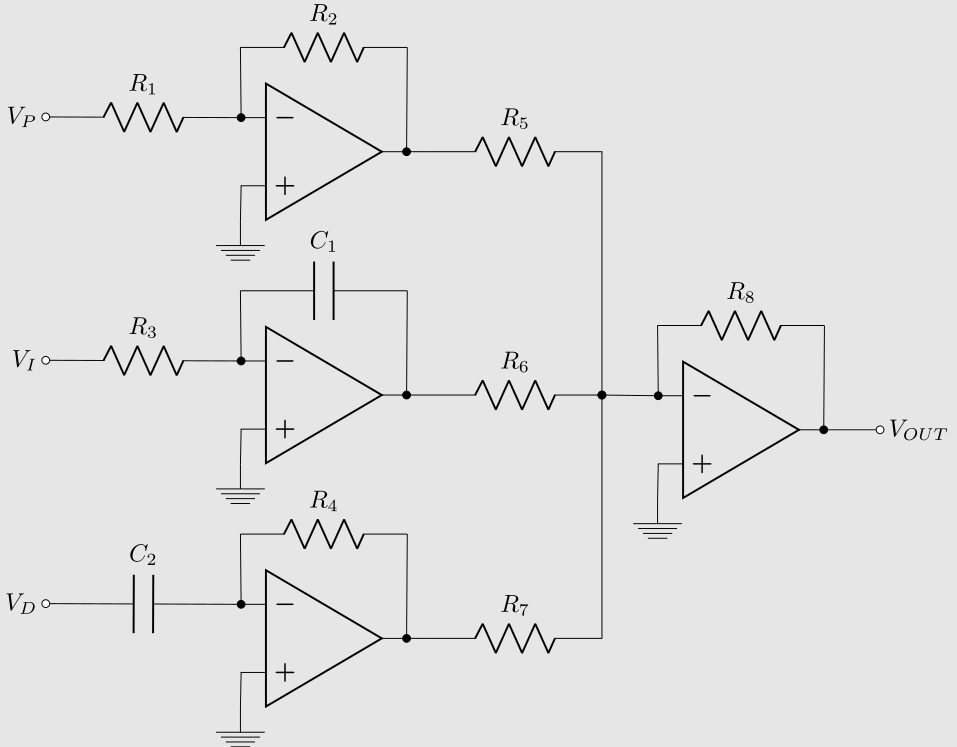
\includegraphics[width=0.9\columnwidth, alt={PID circuit with operational amplifiers.}]{Circuito_PID.png}

                {\tiny \textbf{Attribution:} Galessandroni, \href{https://creativecommons.org/licenses/by-sa/4.0}{CC BY-SA 4.0}, via \href{https://commons.wikimedia.org/wiki/File:Circuito_PID.svg}{Wikimedia Commons}\par}

            \end{figure}
        \end{column}
    \end{columns}
\end{frame}

\subsection{Series Circuits}

\begin{frame}
    \frametitle{Series Circuit Defined}

    \begin{figure}
        \centering
        \resizebox{0.48\linewidth}{!}{
            \begin{circuitikz}[
    american,
    >=latex,
    %>={Latex[length=5mm, width=2mm]},
    alt={A circuit with a DC voltage source, V, and 3 resistors R1, R2, and R2 all in series.}
]

    \draw[
        BakerBlack
    ]
    (0,0)
    to[battery, v<=$V$, invert, color=BakerBlack] ++(0,3)
    to[R=$R_1$, color=BakerBlack] ++(3,0)
    to[R=$R_2$, color=BakerBlack] ++(0,-3)
    to[R=$R_3$, color=BakerBlack] (0,0);

\end{circuitikz}
        }

        \vspace{0.5em}
        {\footnotesize A \emph{series circuit} is a circuit that has only one path for current to follow--if that path is broken, current stops\par}
    \end{figure}
\end{frame}

\begin{frame}
    \frametitle{Resistance in Series}
	\begin{columns}
        \begin{column}{0.48\linewidth}
            \begin{itemize}
                \item Resistance in series \emph{adds}
            \end{itemize}
            \[
                R_T=\sum_{i=1}^{n}R_i=R_1+R_2+\cdots+R_n
            \]
        \end{column}
        \begin{column}{0.48\linewidth}
            \begin{figure}
                \centering
                \resizebox{\columnwidth}{!}{
                    \begin{circuitikz}[
    american,
    >=latex,
    %>={Latex[length=5mm, width=2mm]},
    alt={A circuit with a DC voltage source, V, and 3 resistors R1, R2, and R2 all in series.}
]

    \draw[
        BakerBlack
    ]
    (0,0)
    to[battery, v<=$V$, invert, color=BakerBlack] ++(0,3)
    to[R=$R_1$, color=BakerBlack] ++(3,0)
    to[R=$R_2$, color=BakerBlack] ++(0,-3)
    to[R=$R_3$, color=BakerBlack] (0,0);

\end{circuitikz}
                }
            \end{figure}
        \end{column}
	\end{columns}
\end{frame}

\begin{frame}
    \frametitle{Resistance in Series Example 1}
	\begin{columns}
        \begin{column}{0.48\linewidth}
            \begin{itemize}
                \item What is the total resistance of this circuit?
            \end{itemize}
            % \[
            %     R_T=\sum_{i=1}^{n}R_i=R_1+R_2+\cdots+R_n
            % \]
        \end{column}
        \begin{column}{0.48\linewidth}
            \begin{figure}
                \centering
                \resizebox{\columnwidth}{!}{
                    \begin{circuitikz}[
    american,
    >=latex,
    %>={Latex[length=5mm, width=2mm]},
    alt={A circuit with a DC voltage source, V, and 3 resistors 10 ohm, 5 ohm, and 20 ohm all in series.}
]

    \draw[
        BakerBlack
    ]
    (0,0)
    to[battery, v<=$V$, invert, color=BakerBlack] ++(0,3)
    to[R=$10\,\Omega$, color=BakerBlack] ++(3,0)
    to[R=$5\,\Omega$, color=BakerBlack] ++(0,-3)
    to[R=$20\,\Omega$, color=BakerBlack] (0,0);

\end{circuitikz}
                }
            \end{figure}
        \end{column}
	\end{columns}
\end{frame}

\begin{frame}
    \frametitle{Resistance in Series Example 1 Solution}
	\begin{columns}
        \begin{column}{0.48\linewidth}
            \[
                \begin{aligned}                        
                    R_T&=\sum_{i=1}^{3}R_i=R_1+R_2+R_3\\
                    &=10\,\Omega + 5\,\Omega + 20\,\Omega\\
                    &=35\,\Omega
                \end{aligned}
            \]
        \end{column}
        \begin{column}{0.48\linewidth}
            \begin{figure}
                \centering
                \resizebox{\columnwidth}{!}{
                    \begin{circuitikz}[
    american,
    >=latex,
    %>={Latex[length=5mm, width=2mm]},
    alt={A circuit with a DC voltage source, V, and 3 resistors 10 ohm, 5 ohm, and 20 ohm all in series.}
]

    \draw[
        BakerBlack
    ]
    (0,0)
    to[battery, v<=$V$, invert, color=BakerBlack] ++(0,3)
    to[R=$10\,\Omega$, color=BakerBlack] ++(3,0)
    to[R=$5\,\Omega$, color=BakerBlack] ++(0,-3)
    to[R=$20\,\Omega$, color=BakerBlack] (0,0);

\end{circuitikz}
                }
            \end{figure}
        \end{column}
	\end{columns}
\end{frame}

\begin{frame}
    \frametitle{Resistance in Series Example 2}
	\begin{columns}
        \begin{column}{0.48\linewidth}
            \begin{itemize}
                \item What is the total resistance of this circuit?
            \end{itemize}
            % \[
            %     R_T=\sum_{i=1}^{n}R_i=R_1+R_2+\cdots+R_n
            % \]
        \end{column}
        \begin{column}{0.48\linewidth}
            \begin{figure}
                \centering
                \resizebox{\columnwidth}{!}{
                    \input{../../assets/diagrams/SeriesCircuit_3Resistor_20_5_10.tex}
                }
            \end{figure}
        \end{column}
	\end{columns}
\end{frame}

\begin{frame}
    \frametitle{Resistance in Series Example 2 Solution}
	\begin{columns}
        \begin{column}{0.48\linewidth}
            \[
                \begin{aligned}                        
                    R_T&=\sum_{i=1}^{3}R_i=R_1+R_2+R_3\\
                    &=20\,\Omega + 5\,\Omega + 10\,\Omega\\
                    &=35\,\Omega
                \end{aligned}
            \]

            \begin{itemize}
                \item Order doesn't matter\dots
            \end{itemize}
        \end{column}
        \begin{column}{0.48\linewidth}
            \begin{figure}
                \centering
                \resizebox{\columnwidth}{!}{
                    \input{../../assets/diagrams/SeriesCircuit_3Resistor_20_5_10.tex}
                }
            \end{figure}
        \end{column}
	\end{columns}
\end{frame}

\begin{frame}
    \frametitle{Current in Series}

    \begin{columns}
        \begin{column}{0.48\linewidth}
            \begin{itemize}[<+- | alert@+>]
                \item{One path for current = current is equal at all points}
                \item{Ohm's Law -- current in a series circuit is equal to the voltage divided by the circuit total resistance}
            \end{itemize}
        \end{column}
        \begin{column}{0.48\linewidth}
            \begin{figure}
                \centering
                \resizebox{\columnwidth}{!}{
                    \begin{circuitikz}[
    american,
    >=latex,
    %>={Latex[length=5mm, width=2mm]},
    alt={A circuit with a DC voltage source, V, and 3 resistors R1, R2, and R2 all in series.}
]

    \draw[
        BakerBlack
    ]
    (0,0)
    to[battery, v<=$V$, invert, color=BakerBlack] ++(0,3)
    to[R=$R_1$, color=BakerBlack] ++(3,0)
    to[R=$R_2$, color=BakerBlack] ++(0,-3)
    to[R=$R_3$, color=BakerBlack] (0,0);

    \draw[
        UpNorthGreen,
        ultra thick,
        ->,
        rounded corners=0.25cm
    ]
    (0.5,2)
    -- (0.5,2.5)
    -- (1.5,2.5)
    node[
        anchor=north,
        text=BakerBlack
    ]{$I$};

\end{circuitikz}
                }
            \end{figure}
        \end{column}
	\end{columns}
\end{frame}

\begin{frame}
    \frametitle{Current in Series Example}

    \begin{columns}
        \begin{column}{0.48\linewidth}
            \begin{itemize}[<+- | alert@+>]
                \item What is the total current draw of this circuit?
            \end{itemize}
        \end{column}
        \begin{column}{0.48\linewidth}
            \begin{figure}
                \centering
                \resizebox{\columnwidth}{!}{
                    \begin{circuitikz}[
    american,
    >=latex,
    %>={Latex[length=5mm, width=2mm]},
    alt={A circuit with a DC voltage source, V, and 3 resistors R1, R2, and R2 all in series.}
]

    \draw[
        BakerBlack
    ]
    (0,0)
    to[battery, v<=$24\,\text{V}$, invert, color=BakerBlack] ++(0,3)
    to[R=$10\,\Omega$, color=BakerBlack] ++(3,0)
    to[R=$5\,\Omega$, color=BakerBlack] ++(0,-3)
    to[R=$20\,\Omega$, color=BakerBlack] (0,0);

    \draw[
        UpNorthGreen,
        ultra thick,
        ->,
        rounded corners=0.25cm
    ]
    (0.5,2)
    -- (0.5,2.5)
    -- (1.5,2.5)
    node[
        anchor=north,
        text=BakerBlack
    ]{$I$};

\end{circuitikz}
                }
            \end{figure}
        \end{column}
	\end{columns}
\end{frame}

\begin{frame}
    \frametitle{Current in Series Example Solution}

    \begin{columns}
        \begin{column}{0.48\linewidth}
            \[
                \begin{aligned}
                    R_T&=35\,\Omega\\
                    I&=\frac{E}{R}=\frac{24\,\text{V}}{35\,\Omega}=0.686\,\text{A}
                \end{aligned}
            \]
        \end{column}
        \begin{column}{0.48\linewidth}
            \begin{figure}
                \centering
                \resizebox{\columnwidth}{!}{
                    \begin{circuitikz}[
    american,
    >=latex,
    %>={Latex[length=5mm, width=2mm]},
    alt={A circuit with a DC voltage source, V, and 3 resistors R1, R2, and R2 all in series.}
]

    \draw[
        BakerBlack
    ]
    (0,0)
    to[battery, v<=$24\,\text{V}$, invert, color=BakerBlack] ++(0,3)
    to[R=$10\,\Omega$, color=BakerBlack] ++(3,0)
    to[R=$5\,\Omega$, color=BakerBlack] ++(0,-3)
    to[R=$20\,\Omega$, color=BakerBlack] (0,0);

    \draw[
        UpNorthGreen,
        ultra thick,
        ->,
        rounded corners=0.25cm
    ]
    (0.5,2)
    -- (0.5,2.5)
    -- (1.5,2.5)
    node[
        anchor=north,
        text=BakerBlack
    ]{$I$};

\end{circuitikz}
                }
            \end{figure}
        \end{column}
	\end{columns}
\end{frame}

\begin{frame}
    \frametitle{Voltage in Series}
    \begin{columns}
        \begin{column}{0.48\linewidth}
            \begin{itemize}[<+- | alert@+>]
                \item Resistors work by robbing electrons of their energy
                \item The energy is voltage, this loss in energy causes a \emph{voltage drop} across each resistor
                \item Ohm's Law can be used to calculate the drop
            \end{itemize}
        \end{column}
        \begin{column}{0.48\linewidth}
            \begin{figure}
                \centering
                \resizebox{\columnwidth}{!}{
                    \begin{circuitikz}[
    american,
        voltage dir=RP,
    >=latex,
    %>={Latex[length=5mm, width=2mm]},
    alt={A circuit with a DC voltage source, V, and 3 resistors R1, R2, and R2 all in series.}
]

    \draw[
        BakerBlack
    ]
    (0,0)
    to[battery, v=$24\,\text{V}$, color=BakerBlack] ++(0,4)
    to[R=$10\,\Omega$, v=$V_1$, color=BakerBlack] ++(4,0)
    to[R=$5\,\Omega$, v=$V_2$, color=BakerBlack] ++(0,-4)
    to[R=$20\,\Omega$, v=$V_3$, color=BakerBlack] (0,0);

    \draw[
        UpNorthGreen,
        ultra thick,
        ->,
        rounded corners=0.25cm
    ]
    (0.5,2.5)
    -- (0.5,3)
    -- (1.5,3)
    node[
        anchor=north,
        text=BakerBlack
    ]{$0.686\,\text{A}$};

\end{circuitikz}
                }
            \end{figure}
        \end{column}
	\end{columns}
\end{frame}

\begin{frame}
    \frametitle{Voltage in Series Example}
    \begin{columns}
        \begin{column}{0.48\linewidth}
            \begin{itemize}
                \item What is the voltage drop across each of these resistors?
            \end{itemize}
        \end{column}
        \begin{column}{0.48\linewidth}
            \begin{figure}
                \centering
                \resizebox{\columnwidth}{!}{
                    \begin{circuitikz}[
    american,
        voltage dir=RP,
    >=latex,
    %>={Latex[length=5mm, width=2mm]},
    alt={A circuit with a DC voltage source, V, and 3 resistors R1, R2, and R2 all in series.}
]

    \draw[
        BakerBlack
    ]
    (0,0)
    to[battery, v=$24\,\text{V}$, color=BakerBlack] ++(0,4)
    to[R=$10\,\Omega$, v=$V_1$, color=BakerBlack] ++(4,0)
    to[R=$5\,\Omega$, v=$V_2$, color=BakerBlack] ++(0,-4)
    to[R=$20\,\Omega$, v=$V_3$, color=BakerBlack] (0,0);

    \draw[
        UpNorthGreen,
        ultra thick,
        ->,
        rounded corners=0.25cm
    ]
    (0.5,2.5)
    -- (0.5,3)
    -- (1.5,3)
    node[
        anchor=north,
        text=BakerBlack
    ]{$0.686\,\text{A}$};

\end{circuitikz}
                }
            \end{figure}
        \end{column}
	\end{columns}
\end{frame}

\begin{frame}
    \frametitle{Voltage in Series Example Solution}
    \begin{columns}
        \begin{column}{0.48\linewidth}
            \[
                \begin{aligned}
                    E&=IR\\
                    V_1&=IR_1=\left(0.686\,\text{A}\right)\left(10\,\Omega\right)=6.86\,\text{V}\\
                    V_2&=IR_2=\left(0.686\,\text{A}\right)\left(5\,\Omega\right)=3.43\,\text{V}\\
                    V_3&=IR_3=\left(0.686\,\text{A}\right)\left(20\,\Omega\right)=13.72\,\text{V}\\
                    V_T&=6.86\,\text{V}+3.43\,\text{V}+13.72\,\text{V}=24\,\text{V}
                \end{aligned}
            \]
        \end{column}
        \begin{column}{0.48\linewidth}
            \begin{figure}
                \centering
                \resizebox{\columnwidth}{!}{
                    \begin{circuitikz}[
    american,
        voltage dir=RP,
    >=latex,
    %>={Latex[length=5mm, width=2mm]},
    alt={A circuit with a DC voltage source, V, and 3 resistors R1, R2, and R2 all in series.}
]

    \draw[
        BakerBlack
    ]
    (0,0)
    to[battery, v=$24\,\text{V}$, color=BakerBlack] ++(0,4)
    to[R=$10\,\Omega$, v=$V_1$, color=BakerBlack] ++(4,0)
    to[R=$5\,\Omega$, v=$V_2$, color=BakerBlack] ++(0,-4)
    to[R=$20\,\Omega$, v=$V_3$, color=BakerBlack] (0,0);

    \draw[
        UpNorthGreen,
        ultra thick,
        ->,
        rounded corners=0.25cm
    ]
    (0.5,2.5)
    -- (0.5,3)
    -- (1.5,3)
    node[
        anchor=north,
        text=BakerBlack
    ]{$0.686\,\text{A}$};

\end{circuitikz}
                }
            \end{figure}
        \end{column}
	\end{columns}
\end{frame}

\subsection{Parallel Circuits}

\begin{frame}
    \frametitle{Parallel Circuits}

	\begin{columns}
        \begin{column}{0.48\linewidth}
            \begin{itemize}[<+- | alert@+>]
                \item{Two or more components connected such that there is more than one path for current to take}
                \item{De-energizing one path may leave other paths energized}
            \end{itemize}
        \end{column}
        \begin{column}{0.48\linewidth}
            \begin{figure}
                \centering
                \resizebox{\columnwidth}{!}{
                    \input{../../assets/diagrams/Parallel_3Resistor_Generic.tex}
                }
            \end{figure}
        \end{column}
	\end{columns}
\end{frame}

\begin{frame}
    \frametitle{Voltage in Parallel}

	\begin{columns}
        \begin{column}{0.48\linewidth}
            \begin{itemize}
                \item The voltage across any parallel component is equal to the voltage across all other parallel components
                \item In more complex circuits the V is the voltage in a parallel \emph{leg}, not the supply
            \end{itemize}
            \[V=V_{1}=V_{2}=V_{3}\]
        \end{column}
        \begin{column}{0.48\linewidth}
            \begin{figure}
                \centering
                \resizebox{\columnwidth}{!}{
                    \begin{circuitikz}[
    american,
    voltage dir=RP,
    >=latex,
    %>={Latex[length=5mm, width=2mm]},
    alt={A circuit with a DC voltage source, V, and 3 resistors R1, R2, and R2 all in series.}
]

\draw[
    BakerBlack
]
(0,0)
to[battery=$24\,\text{V}$, color=BakerBlack] ++(0,3)
-- ++(12,0)
coordinate[pos=1/3](r1t)
coordinate[pos=2/3](r2t)
to[R=$R_3$, color=BakerBlack, v=$24\,\text{V}$] ++(0,-3)
--(0,0)
coordinate[pos=1/3](r2b)
coordinate[pos=2/3](r1b);

\draw[
    BakerBlack
]
(r1t)
to[R=$R_1$, color=BakerBlack, v=$24\,\text{V}$, *-*] (r1b);

\draw[
    BakerBlack
]
(r2t)
to[R=$R_2$, color=BakerBlack, v=$24\,\text{V}$, *-*] (r2b);

\end{circuitikz}
                }
            \end{figure}
        \end{column}
	\end{columns}
\end{frame}

\begin{frame}
    \frametitle{Resistance in Parallel}

	\begin{columns}
        \begin{column}{0.48\linewidth}
            \begin{itemize}[<+- | alert@+>]
                \item Resistance in parallel \emph{does not} add, \emph{conductance} does
            \end{itemize}
            \[
                \begin{aligned}
                    G&=\frac{I}{E}=\frac{1}{R}\\
                    \frac{1}{R_{EQ}}&=\sum_{i=1}^{n}\frac{1}{R_i}=\frac{1}{R_1}+\frac{1}{R_2}+ \cdots + \frac{1}{R_n}
                \end{aligned}
            \]
        \end{column}
        \begin{column}{0.48\linewidth}
            \begin{figure}
                \centering
                \resizebox{\columnwidth}{!}{
                    \begin{circuitikz}[
    american,
    voltage dir=RP,
    >=latex,
    %>={Latex[length=5mm, width=2mm]},
    alt={A circuit with a DC voltage source, V, and 3 resistors R1, R2, and R2 all in series.}
]

\draw[
    BakerBlack
]
(0,0)
to[battery=$24\,\text{V}$, color=BakerBlack] ++(0,3)
-- ++(12,0)
coordinate[pos=1/3](r1t)
coordinate[pos=2/3](r2t)
to[R=$R_3$, color=BakerBlack, v=$24\,\text{V}$] ++(0,-3)
--(0,0)
coordinate[pos=1/3](r2b)
coordinate[pos=2/3](r1b);

\draw[
    BakerBlack
]
(r1t)
to[R=$R_1$, color=BakerBlack, v=$24\,\text{V}$, *-*] (r1b);

\draw[
    BakerBlack
]
(r2t)
to[R=$R_2$, color=BakerBlack, v=$24\,\text{V}$, *-*] (r2b);

\end{circuitikz}
                }
            \end{figure}
        \end{column}
	\end{columns}
\end{frame}

\begin{frame}
    \frametitle{Resistance in Parallel Example}

	\begin{columns}
        \begin{column}{0.48\linewidth}
            \begin{itemize}[<+- | alert@+>]
                \item What is the equivalent resistance of this circuit?
            \end{itemize}
        \end{column}
        \begin{column}{0.48\linewidth}
            \begin{figure}
                \centering
                \resizebox{\columnwidth}{!}{
                    \input{../../assets/diagrams/Parallel_3Resistor_10_5_20.tex}
                }
            \end{figure}
        \end{column}
	\end{columns}
\end{frame}

\begin{frame}
    \frametitle{Resistance in Parallel Example Solution}

	\begin{columns}
        \begin{column}{0.48\linewidth}
            \[
                \begin{aligned}
                    \frac{1}{R_{EQ}}&=\sum_{i=1}^{3}\frac{1}{R_i}=\frac{1}{R_1}+\frac{1}{R_2}+ \frac{1}{R_3}\\
                    &=\frac{1}{10\,\Omega}+\frac{1}{5\,\Omega}+\frac{1}{20\,\Omega}\\
                    &=\frac{7}{20\,\Omega}\\
                    R_{EQ}&=\frac{20\,\Omega}{7}=2.857\,\Omega
                \end{aligned}
            \]
        \end{column}
        \begin{column}{0.48\linewidth}
            \begin{figure}
                \centering
                \resizebox{\columnwidth}{!}{
                    \input{../../assets/diagrams/Parallel_3Resistor_10_5_20.tex}
                }
            \end{figure}
        \end{column}
	\end{columns}

    \centering
    {\footnotesize Sanity check: the equivalent resistance of a parallel branch will \emph{always} be lower than the smallest individual resistance\par}
\end{frame}

\begin{frame}
    \frametitle{Current in Parallel}

    \begin{columns}
        \begin{column}{0.48\linewidth}
            \begin{itemize}[<+- | alert@+>]
                \item Remember the definition: parallel circuits have multiple current paths
                \item The current splits every time there's a junction
                \item \emph{How much} it splits is determined by Ohm's Law
            \end{itemize}
        \end{column}
        \begin{column}{0.48\linewidth}
            \begin{figure}
                \centering
                \resizebox{\columnwidth}{!}{
                    \begin{circuitikz}[
    american,
    voltage dir=RP,
    >=latex,
    %>={Latex[length=5mm, width=2mm]},
    alt={A circuit with a DC voltage source, V, and 3 resistors R1, R2, and R2 all in series.}
]

\draw[
    BakerBlack
]
(0,0)
to[battery=$24\,\text{V}$, color=BakerBlack] ++(0,3)
coordinate(btop)
-- ++(12,0)
coordinate[pos=1/3](r1t)
coordinate[pos=2/3](r2t)
coordinate(r3t)
to[R=$20\,\Omega$, color=BakerBlack] ++(0,-3)
coordinate(r3b)
--(0,0)
coordinate[pos=1/3](r2b)
coordinate[pos=2/3](r1b);

\draw[
    BakerBlack
]
(r1t)
to[R=$10\,\Omega$, color=BakerBlack, *-*] (r1b);

\draw[
    BakerBlack
]
(r2t)
to[R=$5\,\Omega$, color=BakerBlack, *-*] (r2b);

\draw[
    UpNorthGreen,
    ultra thick,
    ->
]
($(btop)-(-0.5,0.5)$)
-- ($(r1t)-(0.5,0.5)$)
node[
    midway,
    below,
    text=BakerBlack
]{$I_T$};

\draw[
    UpNorthGreen,
    ultra thick,
    ->
]
($(r1t)-(0.5,1)$)
-- ($(r1b)-(0.5,-1)$)
node[
    midway,
    left,
    text=BakerBlack
]{$I_1$};

\draw[
    UpNorthGreen,
    ultra thick,
    ->
]
($(r2t)-(0.5,1)$)
-- ($(r2b)-(0.5,-1)$)
node[
    midway,
    left,
    text=BakerBlack
]{$I_2$};

\draw[
    UpNorthGreen,
    ultra thick,
    ->
]
($(r3t)-(0.5,1)$)
-- ($(r3b)-(0.5,-1)$)
node[
    midway,
    left,
    text=BakerBlack
]{$I_3$};

\end{circuitikz}
                }
            \end{figure}
        \end{column}
	\end{columns}
\end{frame}

\begin{frame}
    \frametitle{Current in Parallel Example}

    \begin{columns}
        \begin{column}{0.48\linewidth}
            \begin{itemize}[<+- | alert@+>]
                \item What is the current through each resistor in this circuit?
            \end{itemize}
        \end{column}
        \begin{column}{0.48\linewidth}
            \begin{figure}
                \centering
                \resizebox{\columnwidth}{!}{
                    \begin{circuitikz}[
    american,
    voltage dir=RP,
    >=latex,
    %>={Latex[length=5mm, width=2mm]},
    alt={A circuit with a DC voltage source, V, and 3 resistors R1, R2, and R2 all in series.}
]

\draw[
    BakerBlack
]
(0,0)
to[battery=$24\,\text{V}$, color=BakerBlack] ++(0,3)
coordinate(btop)
-- ++(12,0)
coordinate[pos=1/3](r1t)
coordinate[pos=2/3](r2t)
coordinate(r3t)
to[R=$20\,\Omega$, color=BakerBlack] ++(0,-3)
coordinate(r3b)
--(0,0)
coordinate[pos=1/3](r2b)
coordinate[pos=2/3](r1b);

\draw[
    BakerBlack
]
(r1t)
to[R=$10\,\Omega$, color=BakerBlack, *-*] (r1b);

\draw[
    BakerBlack
]
(r2t)
to[R=$5\,\Omega$, color=BakerBlack, *-*] (r2b);

\draw[
    UpNorthGreen,
    ultra thick,
    ->
]
($(btop)-(-0.5,0.5)$)
-- ($(r1t)-(0.5,0.5)$)
node[
    midway,
    below,
    text=BakerBlack
]{$I_T$};

\draw[
    UpNorthGreen,
    ultra thick,
    ->
]
($(r1t)-(0.5,1)$)
-- ($(r1b)-(0.5,-1)$)
node[
    midway,
    left,
    text=BakerBlack
]{$I_1$};

\draw[
    UpNorthGreen,
    ultra thick,
    ->
]
($(r2t)-(0.5,1)$)
-- ($(r2b)-(0.5,-1)$)
node[
    midway,
    left,
    text=BakerBlack
]{$I_2$};

\draw[
    UpNorthGreen,
    ultra thick,
    ->
]
($(r3t)-(0.5,1)$)
-- ($(r3b)-(0.5,-1)$)
node[
    midway,
    left,
    text=BakerBlack
]{$I_3$};

\end{circuitikz}
                }
            \end{figure}
        \end{column}
	\end{columns}
\end{frame}

\begin{frame}
    \frametitle{Current in Parallel Example Solution}

    \begin{columns}
        \begin{column}{0.48\linewidth}
            \[
                \begin{aligned}
                    I_1&=\frac{E}{R_1}=\frac{24\,\text{V}}{10\,\Omega}=2.4\,\text{A}\\
                    I_2&=\frac{E}{R_2}=\frac{24\,\text{V}}{5\,\Omega}=4.8\,\text{A}\\
                    I_3&=\frac{E}{R_3}=\frac{24\,\text{V}}{5\,\Omega}=1.2\,\text{A}
                \end{aligned}
            \]
        \end{column}
        \begin{column}{0.48\linewidth}
            \begin{figure}
                \centering
                \resizebox{\columnwidth}{!}{
                    \input{../../assets/diagrams/Parallel_3Resistor_10_5_20_CurrentArrows_Solved.tex}
                }
            \end{figure}
        \end{column}
	\end{columns}
\end{frame}

\section{Electrical Safety}

\begin{frame}
    \frametitle{Electric Shock}
	\centering
    \href{https://www.yout-ube.com/watch?v=y_cWTWB-N_I}{Current Vs Voltage: How Much Current Can Kill You?} (5:21) 

    {\scriptsize \href{https://www.yout-ube.com/watch?v=y_cWTWB-N_I}{https://www.yout-ube.com/watch?v=y\_cWTWB-N\_I}}
\end{frame}

\begin{frame}
    \frametitle{Arc Flash}
    \centering
	\href{https://www.yout-ube.com/watch?v=6hpE5LYj-CY}{Electrical Arc Flash Demonstration} (1:17) 

    {\scriptsize \href{https://www.yout-ube.com/watch?v=6hpE5LYj-CY}{https://www.yout-ube.com/watch?v=6hpE5LYj-CY}}
\end{frame}

\subsection{Electrical Standards}

\begin{frame}
    \frametitle{National Fire Protection Association}

	\begin{columns}
        \begin{column}{0.48\linewidth}
            \begin{itemize}[<+- | alert@+>]
                \item{Began as a safety organization focused on preventing fires in the workplace}
                \item{Currently publishes several important electrical standards}
            \end{itemize}
        \end{column}
        \begin{column}{0.48\linewidth}
            \begin{figure}
                \centering
                
\includegraphics[width=0.75\columnwidth, alt={Official logo of the National Fire Protection Association, known as NFPA. The logo features a red flame centered inside a thick black square frame with an open bottom, with the bold black letters NFPA printed directly underneath on a plain white background.}]{NFPA-Logo-RBG-2015.png}
                
                {\tiny NFPA logo is a registered trademark of the National Fire Protection Association. Used here for educational and identification purposes under nominative fair use.\par}
            \end{figure}
        \end{column}
	\end{columns}
\end{frame}

\begin{frame}
    \frametitle{NFPA Standards}

	\begin{columns}
        \begin{column}{0.48\linewidth}
            \begin{itemize}[<+- | alert@+>]
                \item{NFPA 70 -- National Electric Code (NEC)}
                \item{NFPA 70e -- Standard for Electrical Safety in the Workplace}
                \item{NFPA 79 -- Electrical Standards for Industrial Machinery}
            \end{itemize}
        \end{column}
        \begin{column}{0.48\linewidth}
            \begin{figure}
                \centering
                
\includegraphics[width=0.75\columnwidth, alt={Official logo of the National Fire Protection Association, known as NFPA. The logo features a red flame centered inside a thick black square frame with an open bottom, with the bold black letters NFPA printed directly underneath on a plain white background.}]{NFPA-Logo-RBG-2015.png}
                
                {\tiny NFPA logo is a registered trademark of the National Fire Protection Association. Used here for educational and identification purposes under nominative fair use.\par}
            \end{figure}
        \end{column}
	\end{columns}
\end{frame}

\begin{frame}
    \frametitle{NFPA Free Access}

	\begin{columns}
        \begin{column}{0.48\linewidth}
            \begin{itemize}[<+- | alert@+>]
                \item{Hard copies of these standards can be expensive}
                \item{\href{http://www.nfpa.org}{NFPA's website} offers free viewing of all standards}
                \item{\textbf{HIGHLY} recommend creating a free account}
            \end{itemize}
        \end{column}
        \begin{column}{0.48\linewidth}
            \begin{figure}
                \centering
                
\includegraphics[width=0.75\columnwidth, alt={Official logo of the National Fire Protection Association, known as NFPA. The logo features a red flame centered inside a thick black square frame with an open bottom, with the bold black letters NFPA printed directly underneath on a plain white background.}]{NFPA-Logo-RBG-2015.png}
                
                {\tiny NFPA logo is a registered trademark of the National Fire Protection Association. Used here for educational and identification purposes under nominative fair use.\par}
            \end{figure}
        \end{column}
	\end{columns}
\end{frame}

\subsection{Electrical Enclosures}

\begin{frame}
    \frametitle{Electrical Enclosures}
    
        \begin{columns}
        \begin{column}{0.48\linewidth}
            \begin{itemize}[<+- | alert@+>]
                \item{Enclosures are selected based on their use scenario}
                \item{Two standards for rating enclosures:}
                \begin{itemize}
                    \item{National Electronics Manufacturers Association (NEMA)}
                    \item{International Electrotechnical Commission (IEC)}
                \end{itemize}
            \end{itemize}
        \end{column}
        \begin{column}{0.48\linewidth}
            \begin{figure}
                \centering
                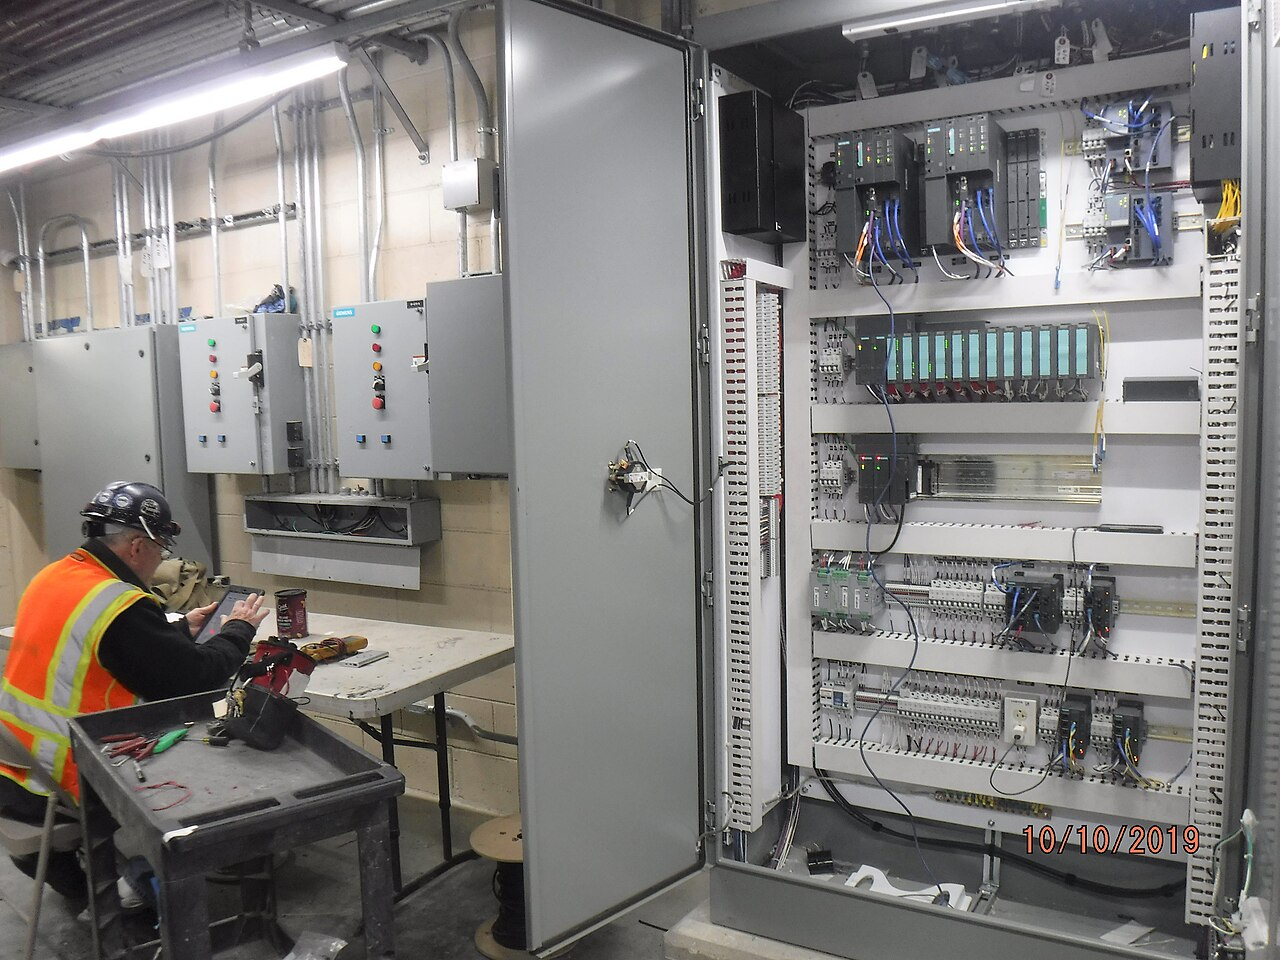
\includegraphics[width=\columnwidth, alt={A technician wearing a hard hat and high-visibility safety vest sitting at a table in a utility room, operating a digital tablet. Next to him stands a large, open electrical control panel filled with organized wiring, circuit modules, and industrial control equipment. Additional grey electrical boxes and conduit pipes line the concrete wall in the background.}]{Testing_the_tunnel_ventilation.jpg}

                {\tiny \textbf{Attribution:} MTA Capital Construction Mega Projects, \href{https://creativecommons.org/licenses/by/2.0}{CC BY 2.0}, via \href{https://commons.wikimedia.org/wiki/File:Testing_the_tunnel_ventilation_control_system_at_a_vent_facility_in_Queens._10-10-2019_(48881721918).jpg}{Wikimedia Commons}\par}
            \end{figure}
        \end{column}
	\end{columns}
\end{frame}

\begin{frame}
    \frametitle{NEMA Enclosure Ratings (1 of 4)}

	\begin{columns}
        \begin{column}{0.48\linewidth}
            \begin{description}[<+- | alert@+>]
                \item[ALL]{ ratings protect personnel from hazardous parts}
                \begin{itemize}
                    \item{It's a box -- you can't touch the stuff inside it}
                \end{itemize}
            \end{description}
        \end{column}
        \begin{column}{0.48\linewidth}
            \begin{figure}
                \centering
                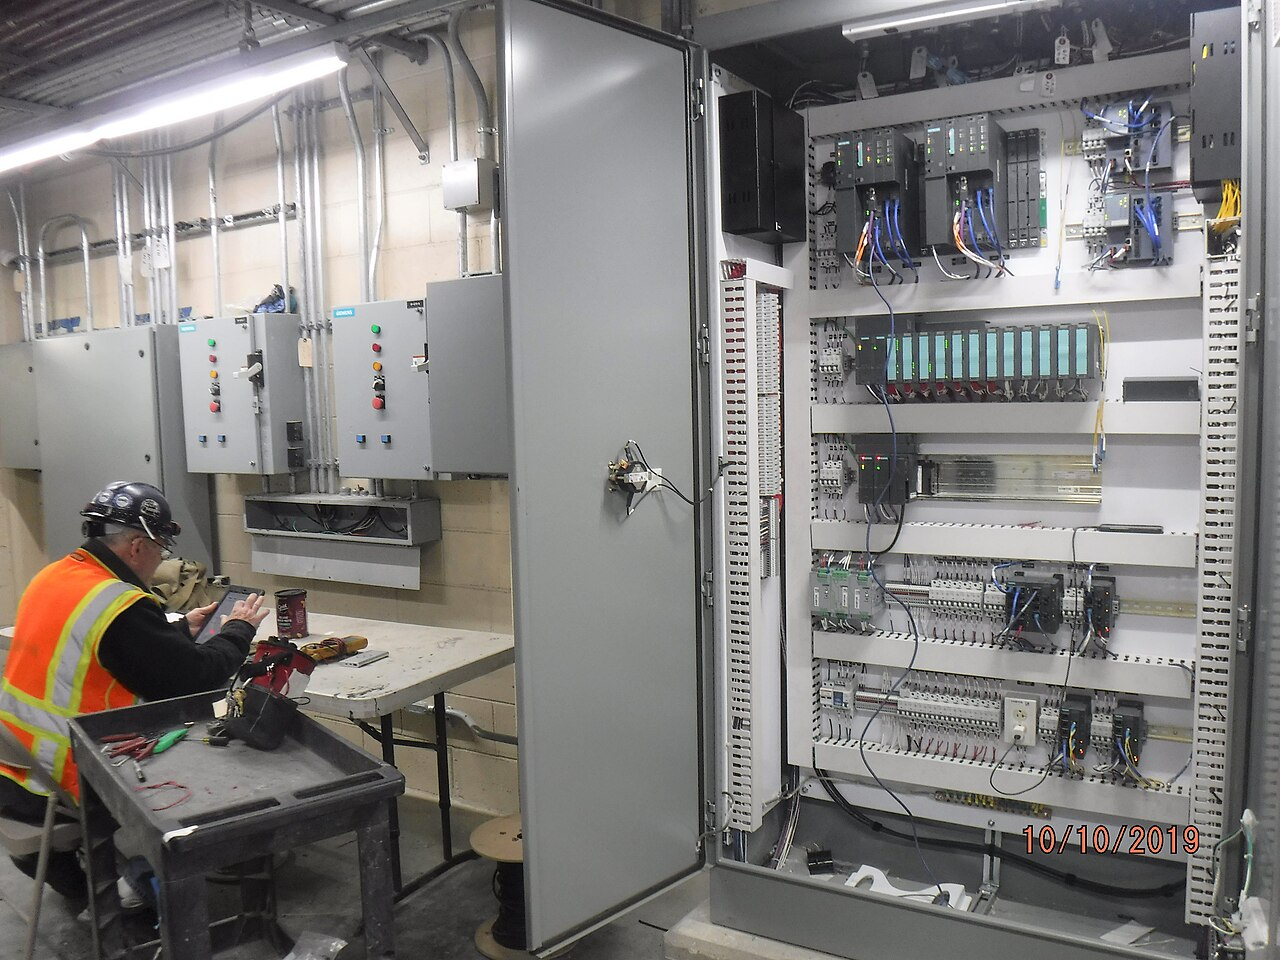
\includegraphics[width=\columnwidth, alt={A technician wearing a hard hat and high-visibility safety vest sitting at a table in a utility room, operating a digital tablet. Next to him stands a large, open electrical control panel filled with organized wiring, circuit modules, and industrial control equipment. Additional grey electrical boxes and conduit pipes line the concrete wall in the background.}]{Testing_the_tunnel_ventilation.jpg}

                {\tiny \textbf{Attribution:} MTA Capital Construction Mega Projects, \href{https://creativecommons.org/licenses/by/2.0}{CC BY 2.0}, via \href{https://commons.wikimedia.org/wiki/File:Testing_the_tunnel_ventilation_control_system_at_a_vent_facility_in_Queens._10-10-2019_(48881721918).jpg}{Wikimedia Commons}\par}
            \end{figure}
        \end{column}
	\end{columns}
\end{frame}

\begin{frame}
    \frametitle{NEMA Enclosure Ratings (2 of 4)}

	\begin{columns}
        \begin{column}{0.48\linewidth}
            \begin{description}[<+- | alert@+>]
                \item[R]{added to rating means it includes a drain hole for water}
                \item[X]{added to rating means it is corrosion resistant (stainless, plastic, fiberglass, etc.)}
            \end{description}
        \end{column}
        \begin{column}{0.48\linewidth}
            \begin{figure}
                \centering
                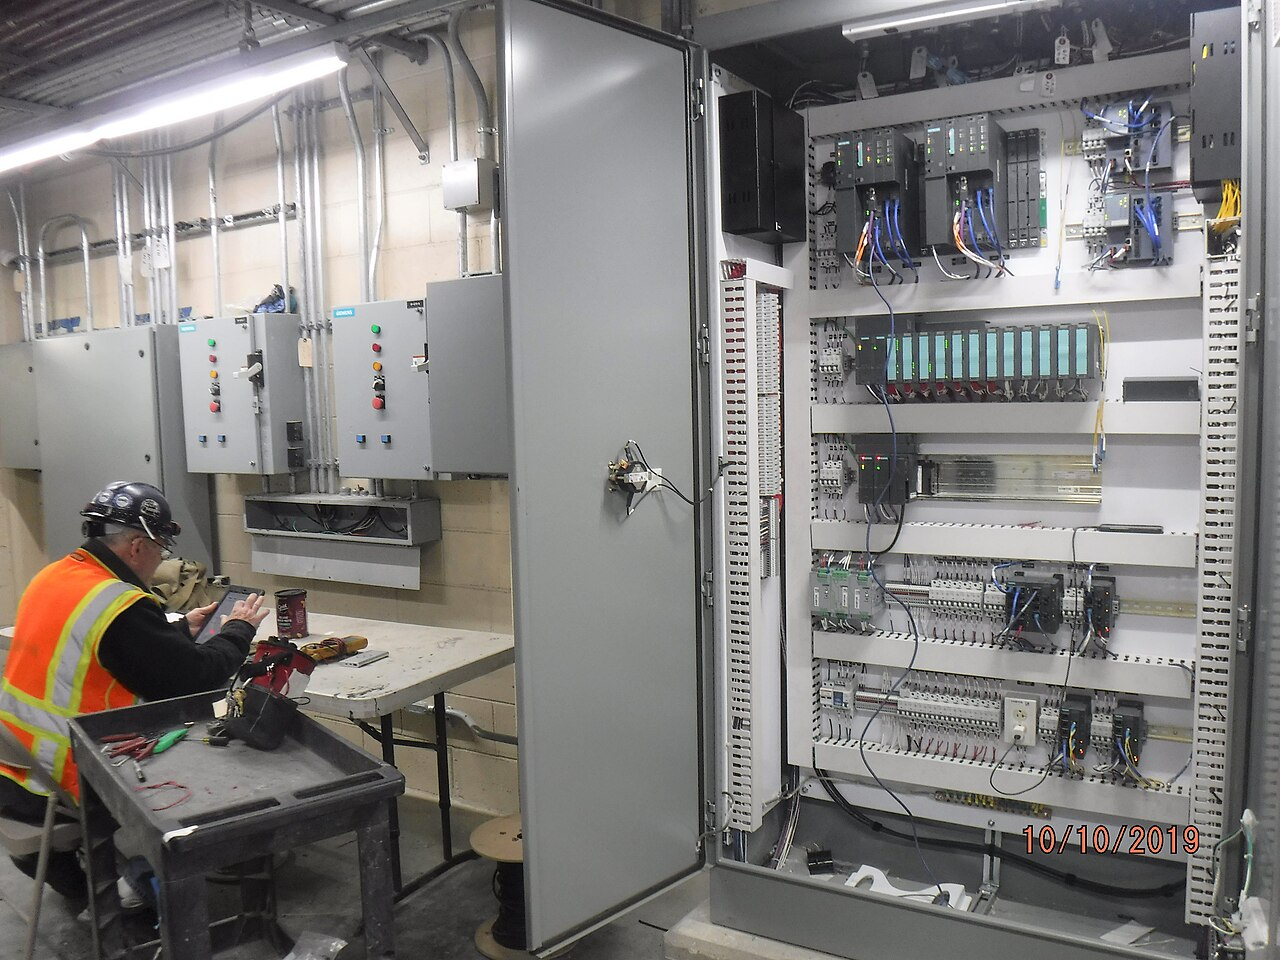
\includegraphics[width=\columnwidth, alt={A technician wearing a hard hat and high-visibility safety vest sitting at a table in a utility room, operating a digital tablet. Next to him stands a large, open electrical control panel filled with organized wiring, circuit modules, and industrial control equipment. Additional grey electrical boxes and conduit pipes line the concrete wall in the background.}]{Testing_the_tunnel_ventilation.jpg}

                {\tiny \textbf{Attribution:} MTA Capital Construction Mega Projects, \href{https://creativecommons.org/licenses/by/2.0}{CC BY 2.0}, via \href{https://commons.wikimedia.org/wiki/File:Testing_the_tunnel_ventilation_control_system_at_a_vent_facility_in_Queens._10-10-2019_(48881721918).jpg}{Wikimedia Commons}\par}
            \end{figure}
        \end{column}
	\end{columns}
\end{frame}

\begin{frame}
    \frametitle{NEMA Enclosure Ratings (3 of 4)}

	\begin{columns}
        \begin{column}{0.48\linewidth}
            \begin{block}{NEMA 1}
                \begin{itemize}[<+- | alert@+>]
                    \pause
                    \item{Indoor use only}
                    \item{Protects equipment from falling dust}
                \end{itemize}
            \end{block}
            \pause
            \begin{block}{NEMA 3}
                \begin{itemize}[<+- | alert@+>]
                    \pause
                    \item{Indoor/outdoor}
                    \item{Protects from falling and windblown dust}
                    \item{Protects from incidental weather}
                \end{itemize}
            \end{block}
        \end{column}
        \begin{column}{0.48\linewidth}
            \begin{figure}
                \centering
                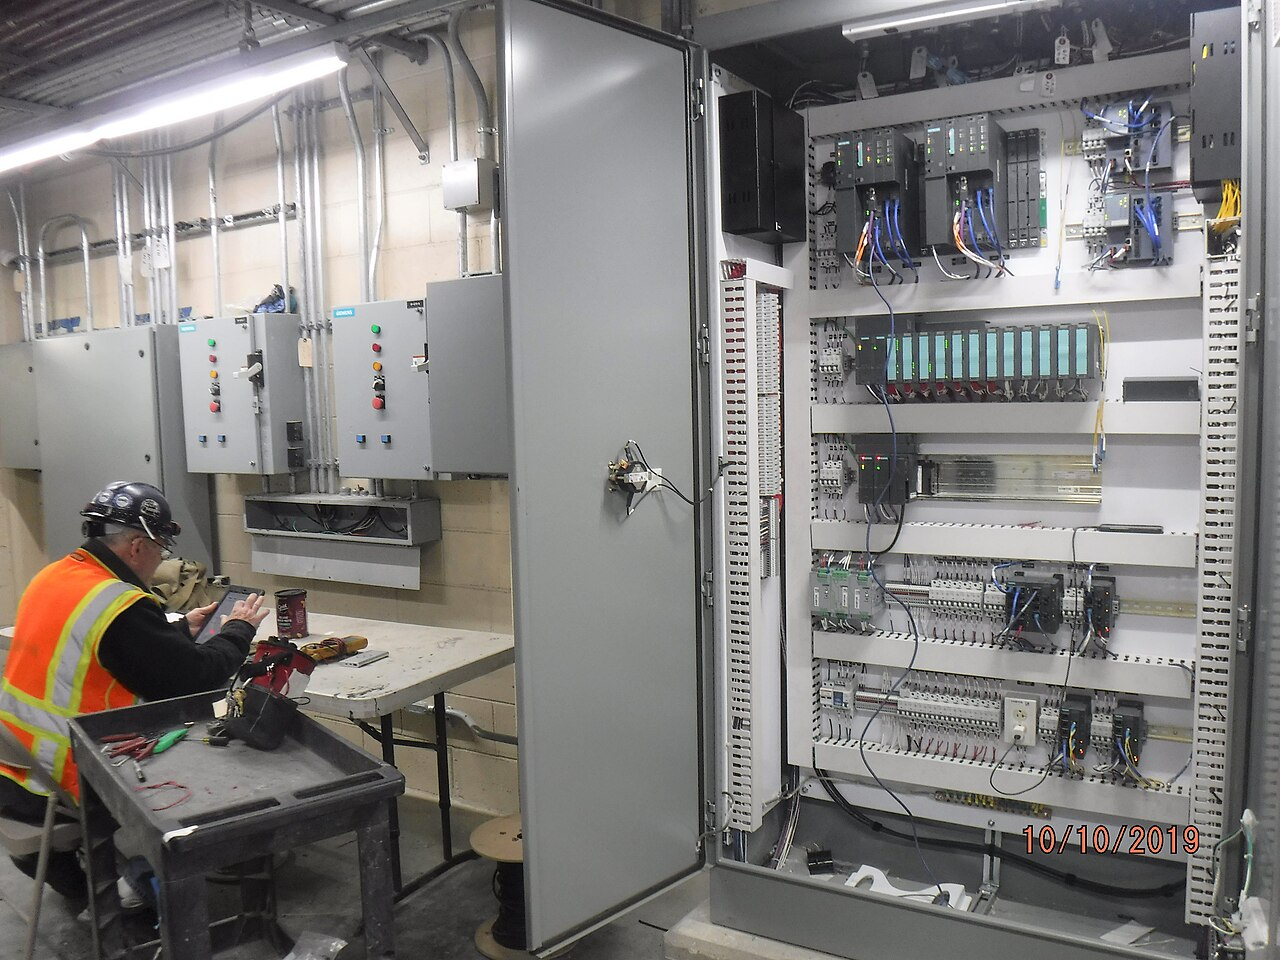
\includegraphics[width=\columnwidth, alt={A technician wearing a hard hat and high-visibility safety vest sitting at a table in a utility room, operating a digital tablet. Next to him stands a large, open electrical control panel filled with organized wiring, circuit modules, and industrial control equipment. Additional grey electrical boxes and conduit pipes line the concrete wall in the background.}]{Testing_the_tunnel_ventilation.jpg}

                {\tiny \textbf{Attribution:} MTA Capital Construction Mega Projects, \href{https://creativecommons.org/licenses/by/2.0}{CC BY 2.0}, via \href{https://commons.wikimedia.org/wiki/File:Testing_the_tunnel_ventilation_control_system_at_a_vent_facility_in_Queens._10-10-2019_(48881721918).jpg}{Wikimedia Commons}\par}
            \end{figure}
        \end{column}
	\end{columns}
\end{frame}

\begin{frame}
    \frametitle{NEMA Enclosure Ratings (4 of 4)}

	\begin{columns}
        \begin{column}{0.48\linewidth}
            \begin{itemize}[<+- | alert@+>]
                \pause
                \item{Indoor/outdoor}
                \item{Protects from incidental and hose directed water}
            \end{itemize}
        \end{column}
        \begin{column}{0.48\linewidth}
            \begin{figure}
                \centering
                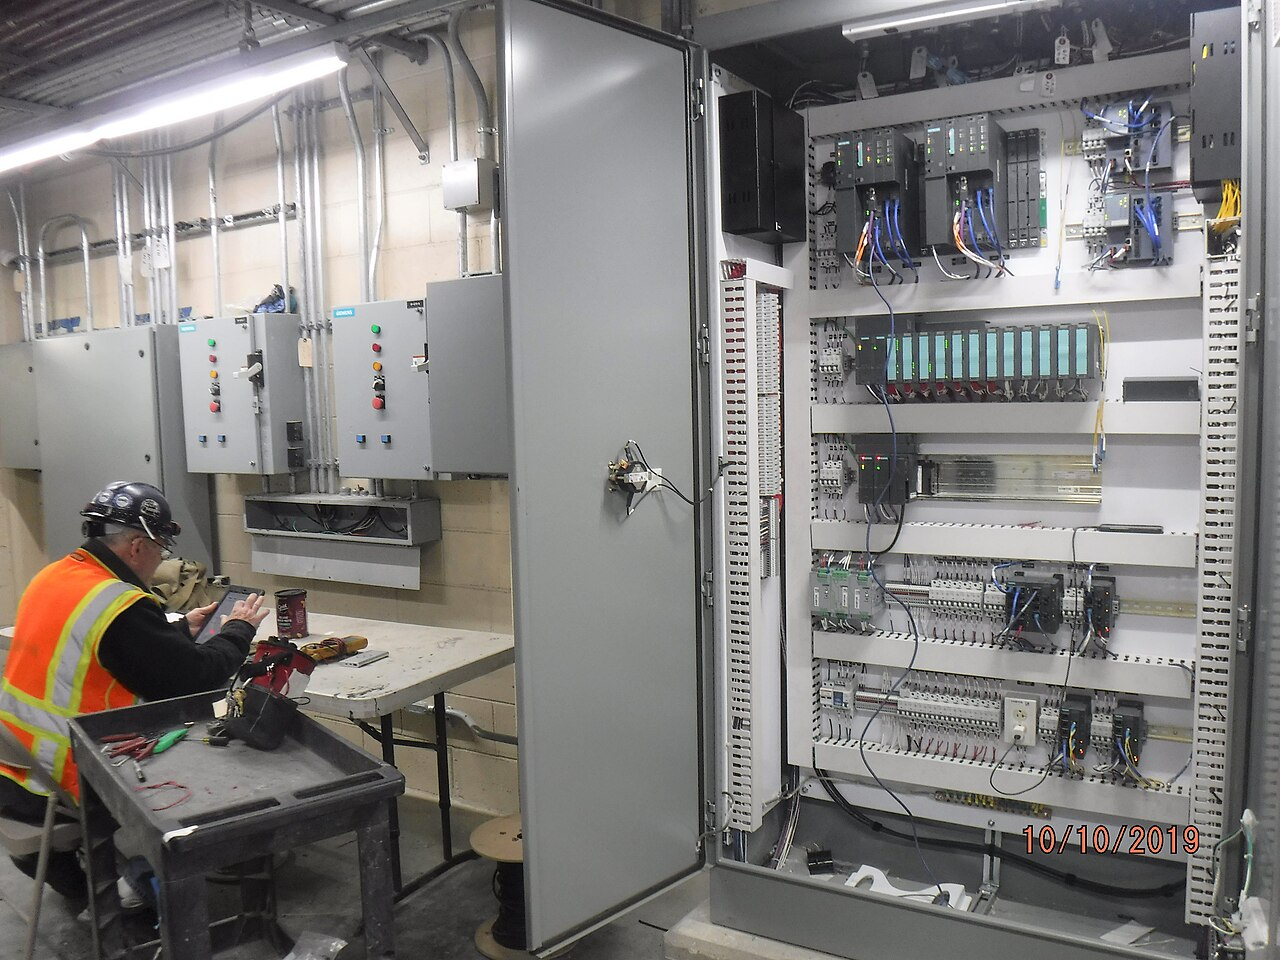
\includegraphics[width=\columnwidth, alt={A technician wearing a hard hat and high-visibility safety vest sitting at a table in a utility room, operating a digital tablet. Next to him stands a large, open electrical control panel filled with organized wiring, circuit modules, and industrial control equipment. Additional grey electrical boxes and conduit pipes line the concrete wall in the background.}]{Testing_the_tunnel_ventilation.jpg}

                {\tiny \textbf{Attribution:} MTA Capital Construction Mega Projects, \href{https://creativecommons.org/licenses/by/2.0}{CC BY 2.0}, via \href{https://commons.wikimedia.org/wiki/File:Testing_the_tunnel_ventilation_control_system_at_a_vent_facility_in_Queens._10-10-2019_(48881721918).jpg}{Wikimedia Commons}\par}
            \end{figure}
        \end{column}
	\end{columns}
\end{frame}

\begin{frame}
    \frametitle{IEC Enclosure Ratings}

	\begin{columns}
        \begin{column}{0.48\linewidth}
            \begin{itemize}[<+- | alert@+>]
                \item{Ingress Protection (IP) rating}
                \item{Defines sealing effectiveness against foreign bodies (solids) and moisture}
                \begin{itemize}
                    \item{First digit = intrusion protection (solids)}
                    \item{Second digit = moisture protection}			
                \end{itemize}
                \item{X means the enclosure is not rated for that spec}
            \end{itemize}
        \end{column}
        \begin{column}{0.48\linewidth}
            \begin{figure}
                \centering
                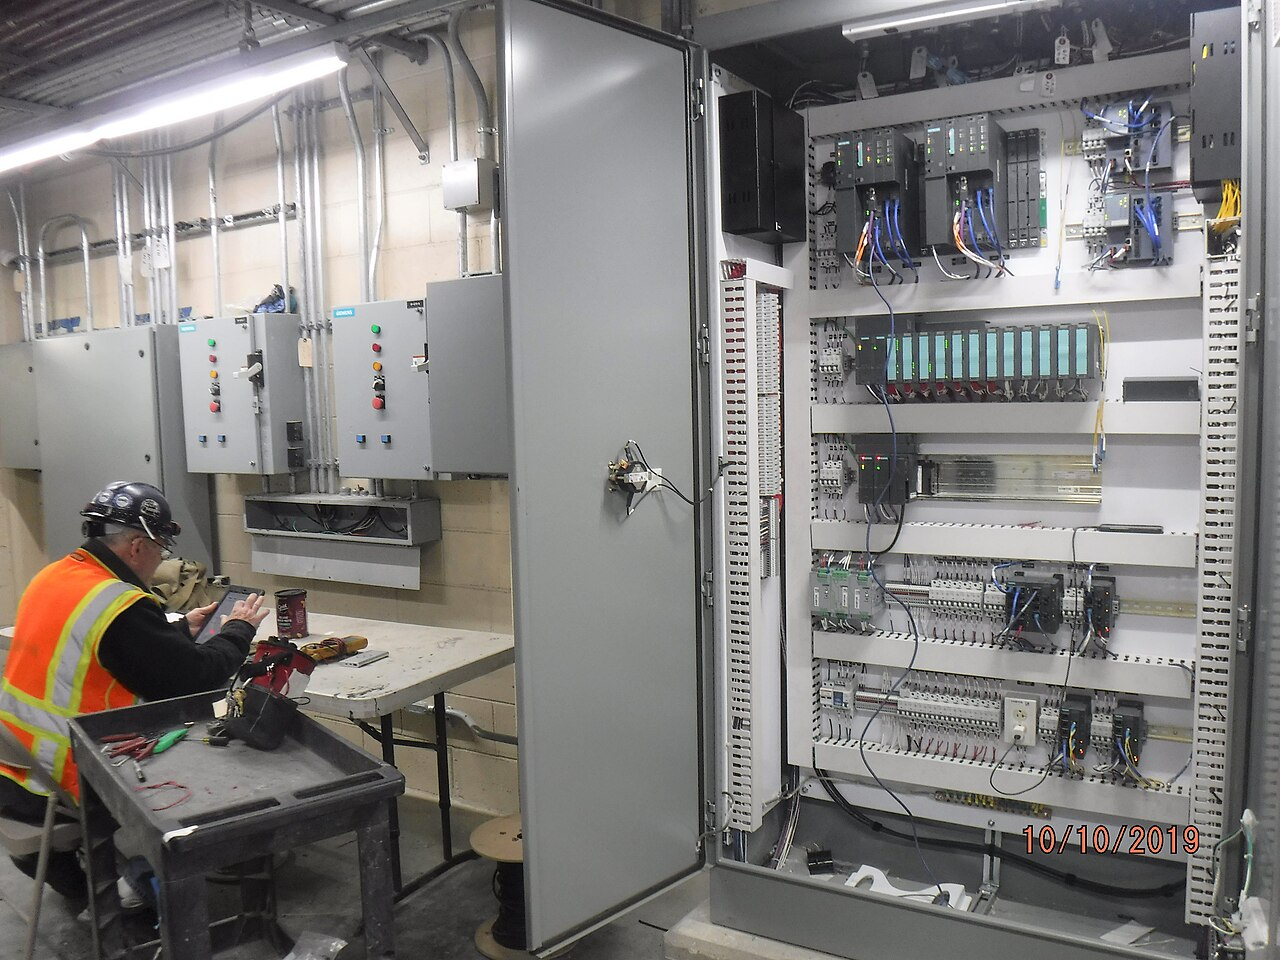
\includegraphics[width=\columnwidth, alt={A technician wearing a hard hat and high-visibility safety vest sitting at a table in a utility room, operating a digital tablet. Next to him stands a large, open electrical control panel filled with organized wiring, circuit modules, and industrial control equipment. Additional grey electrical boxes and conduit pipes line the concrete wall in the background.}]{Testing_the_tunnel_ventilation.jpg}

                {\tiny \textbf{Attribution:} MTA Capital Construction Mega Projects, \href{https://creativecommons.org/licenses/by/2.0}{CC BY 2.0}, via \href{https://commons.wikimedia.org/wiki/File:Testing_the_tunnel_ventilation_control_system_at_a_vent_facility_in_Queens._10-10-2019_(48881721918).jpg}{Wikimedia Commons}\par}
            \end{figure}
        \end{column}
	\end{columns}
\end{frame}

\begin{frame}
    \frametitle{IP Ratings -- Intrusion Protection}

	\begin{columns}
        \begin{column}{0.48\linewidth}
            \begin{description}[<+- | alert@+>]
                \item[0]{No protection}
                \item[1]{>50mm diameter (hands)}
                \item[2]{<80mm length, >12mm diameter (fingers)}
                \item[3]{>2.5mm diameter (tools, wires)}
            \end{description}
        \end{column}
        \begin{column}{0.48\linewidth}
            \begin{description}[<+- | alert@+>]
                \item[4]{>1mm diameter (wires, nails, etc.)}
                \item[5]{Partial protection against dust}
                \item[6]{Totally dust tight}
            \end{description}
        \end{column}
	\end{columns}
\end{frame}

\begin{frame}
    \frametitle{IP Ratings -- Moisture Protection}

	\begin{columns}
        \begin{column}{0.48\linewidth}
            \begin{description}[<+- | alert@+>]
                \item[0]{No protection}
                \item[1]{Vertically falling droplets}
                \item[2]{Droplets up to 15\textdegree from vertical}
                \item[3]{Spray up to 60\textdegree from vertical}
                \item[4]{Splashes from all directions}
                \item[5]{Low pressure jets, all directions}
            \end{description}
        \end{column}
        \begin{column}{0.48\linewidth}
            \begin{description}[<+- | alert@+>]
                \item[6]{Direct, high pressure jets}
                \item[7]{Full immersion up to 30 min at 1m}
                \item[8]{Extended immersion at high pressure}
                \item[9]{High pressure, high temperature jets}
            \end{description}
        \end{column}
	\end{columns}
\end{frame}

\subsection{Grounding and Bonding}

\begin{frame}
    \frametitle{Grounding}

	\begin{columns}
        \begin{column}{0.48\linewidth}
            \begin{itemize}[<+- | alert@+>]
                \item{Grounding -- the connection of all non-current carrying components to the Earth}
                \item{Earth is a giant electrical reservoir}
                \begin{itemize}
                    \item{Readily absorbs stray electricity}
                    \item{No stray electricity = no electrical shock}
                \end{itemize}
            \end{itemize}
        \end{column}
        \begin{column}{0.48\linewidth}
            \begin{figure}
                \centering
                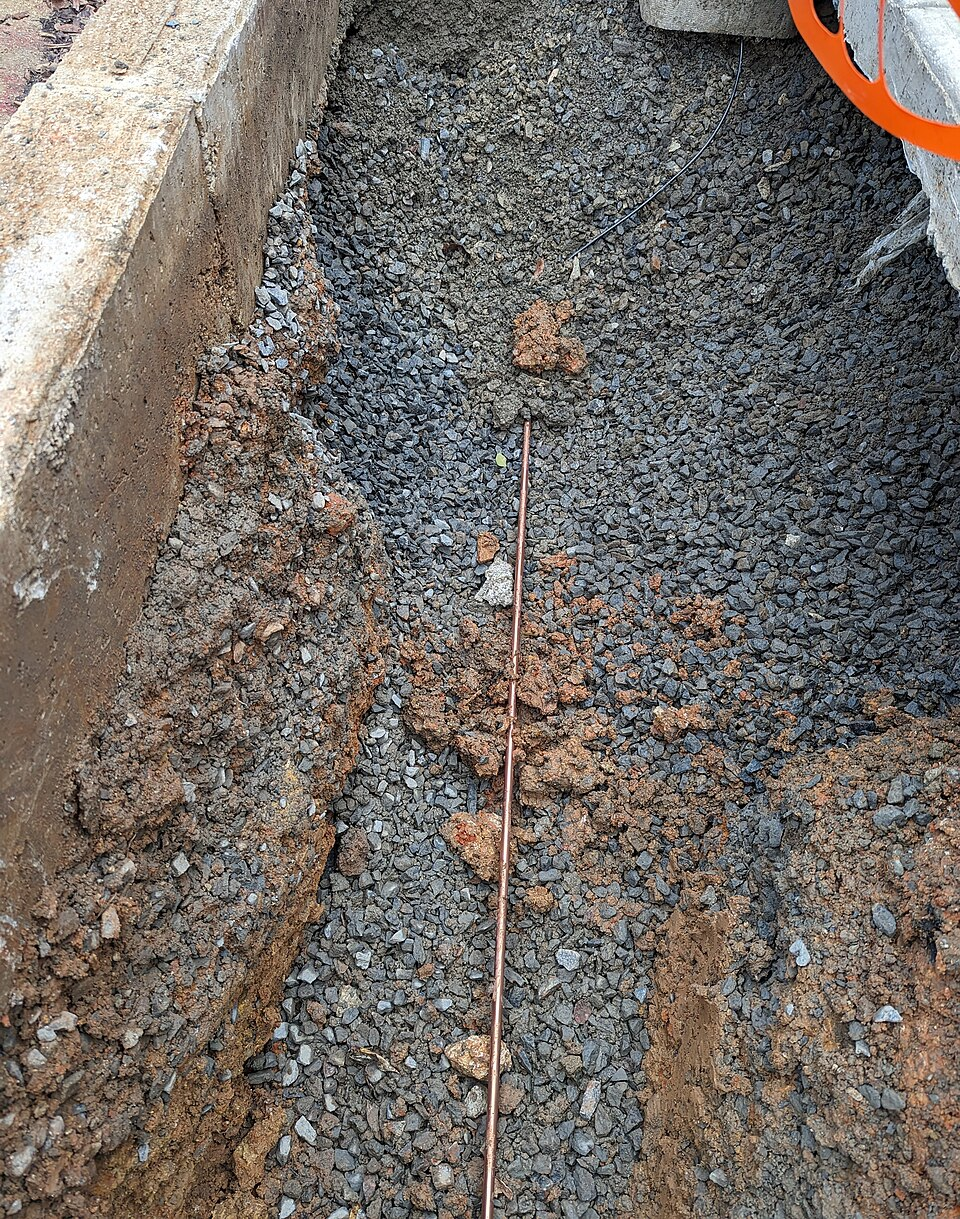
\includegraphics[width=0.75\columnwidth, alt={A copper grounding rod installed horizontally along the bottom of a narrow dirt and gravel trench next to a concrete wall structure. A black wire extends into the trench near the far end, with dirt and coarse gravel partially covering the rod.}]{Ground_rod_installation.jpg}
                
                {\tiny \textbf{Attribution:} Anibal Maysonet, \href{https://creativecommons.org/licenses/by-sa/4.0}{CC BY-SA 4.0}, via \href{https://commons.wikimedia.org/wiki/File:Ground_rod_installation.jpg}{Wikimedia Commons}\par}
            \end{figure}
        \end{column}
	\end{columns}
\end{frame}

\begin{frame}
    \frametitle{Bonding}

	\begin{columns}
        \begin{column}{0.48\linewidth}
            \begin{itemize}[<+- | alert@+>]
                \item{Bonding -- the connection of two separate non-current carrying components to one another}
                \item{Grounding cannot always be used}
                \item{Reduces risk of shock by keeping both components at same potential}
            \end{itemize}
        \end{column}
        \begin{column}{0.48\linewidth}
            \begin{figure}
                \centering
                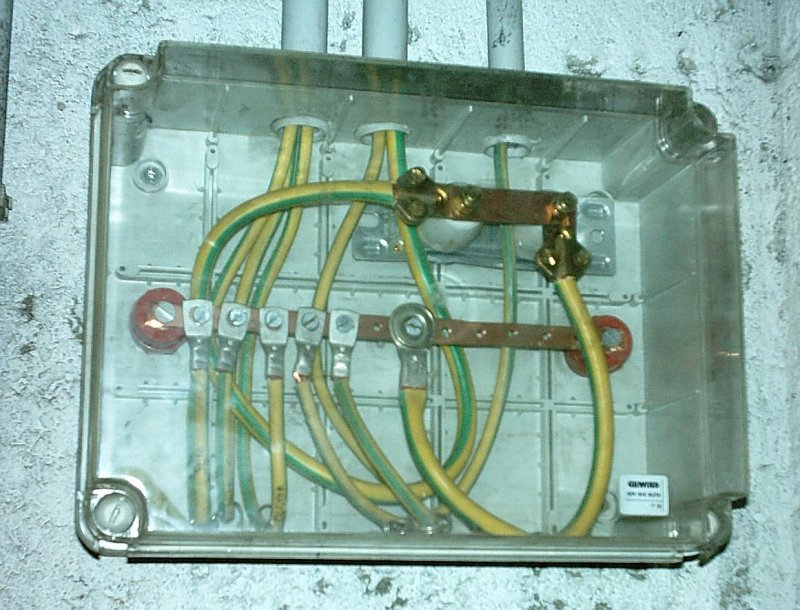
\includegraphics[width=\columnwidth]{Equipotential_bonding_box.jpg}
                
                {\tiny \textbf{Attribution:} Guam\textasciitilde commonswiki, \href{https://creativecommons.org/licenses/by-sa/3.0}{CC BY-SA 3.0}, via \href{https://commons.wikimedia.org/wiki/File:Equipotential_bonding_box.jpg}{Wikimedia Commons}\par}
            \end{figure}
        \end{column}
	\end{columns}
\end{frame}

\begin{frame}
    \frametitle{Electrical Noise}
	\begin{columns}
        \begin{column}{0.48\linewidth}
            \begin{itemize}[<+- | alert@+>]
                \item Any unwanted signal on an electrical component
                \item Not just power wires--communication wires are \emph{especially} noise prone
            \end{itemize}
        \end{column}
        \begin{column}{0.48\linewidth}
            \begin{figure}
                \centering
                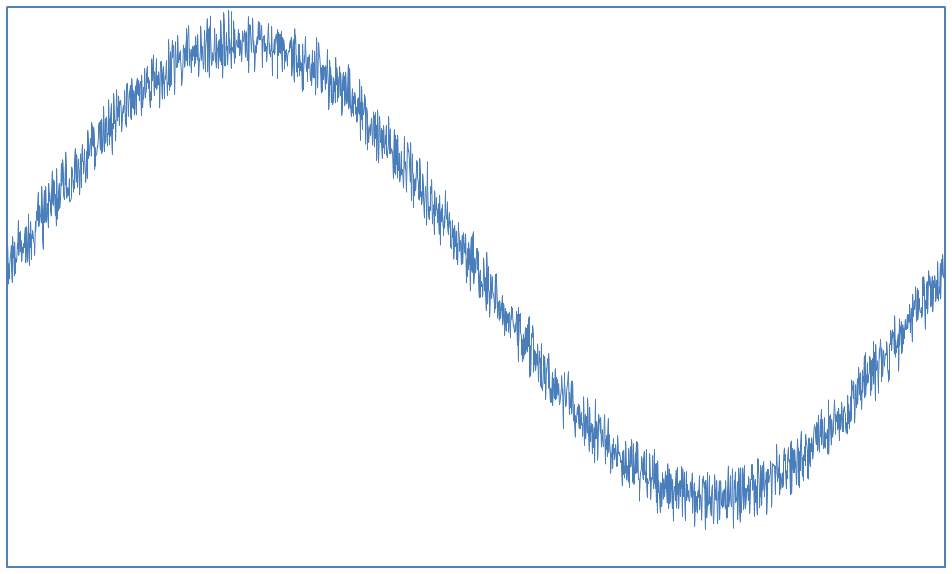
\includegraphics[width=\columnwidth]{Senal4bitsDitherAnalogica1.png}
                
                {\tiny \textbf{Attribution:} Jmcalderon, Public domain, via \href{https://commons.wikimedia.org/wiki/File:Senal4bitsDitherAnalogica1.png}{Wikimedia Commons}\par}
            \end{figure}
        \end{column}
	\end{columns}
\end{frame}

\begin{frame}
    \frametitle{Mitigating Noise}
	\begin{columns}
        \begin{column}{0.48\linewidth}
            \begin{itemize}[<+- | alert@+>]
                \item{PLCs should be places away from noise generating devices}
                \begin{itemize}
                    \item{Motors, starters, welders, etc.}
                \end{itemize}
                \item{AC and DC conductors should be separated}
                \begin{itemize}
                    \item{If they must cross, \textbf{ALWAYS} cross at 90\textdegree}
                \end{itemize}
            \end{itemize}
        \end{column}
        \begin{column}{0.48\linewidth}
            \begin{figure}
                \centering
                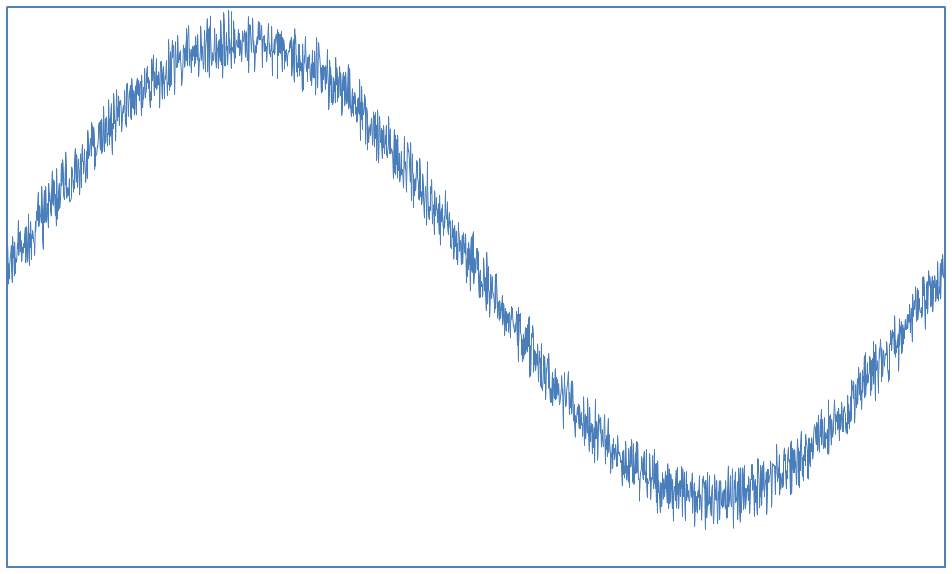
\includegraphics[width=\columnwidth]{Senal4bitsDitherAnalogica1.png}
                
                {\tiny \textbf{Attribution:} Jmcalderon, Public domain, via \href{https://commons.wikimedia.org/wiki/File:Senal4bitsDitherAnalogica1.png}{Wikimedia Commons}\par}
            \end{figure}
        \end{column}
	\end{columns}
\end{frame}

\begin{frame}
    \frametitle{Noise and Safety (1 of 2)}

	\centering
    Why is noise in the safety section of this presentation?
\end{frame}

\begin{frame}
    \frametitle{Noise and Safety (2 of 2)}

	\centering
    If the noise is severe enough it can cause false signals to the PLC--could cause a machine to move when it's not supposed to
\end{frame}

\subsection{Personal Protective Equipment}

\begin{frame}
    \frametitle{Protective Clothing}
	\begin{columns}
        \begin{column}{0.48\linewidth}
            \begin{itemize}[<+- | alert@+>]
                \item{NFPA 70e requires employees to wear flame resistant (FR) clothing whenever exposure to arc flash is possible}
            \end{itemize}
        \end{column}
        \begin{column}{0.48\linewidth}
            \begin{figure}
                \centering
                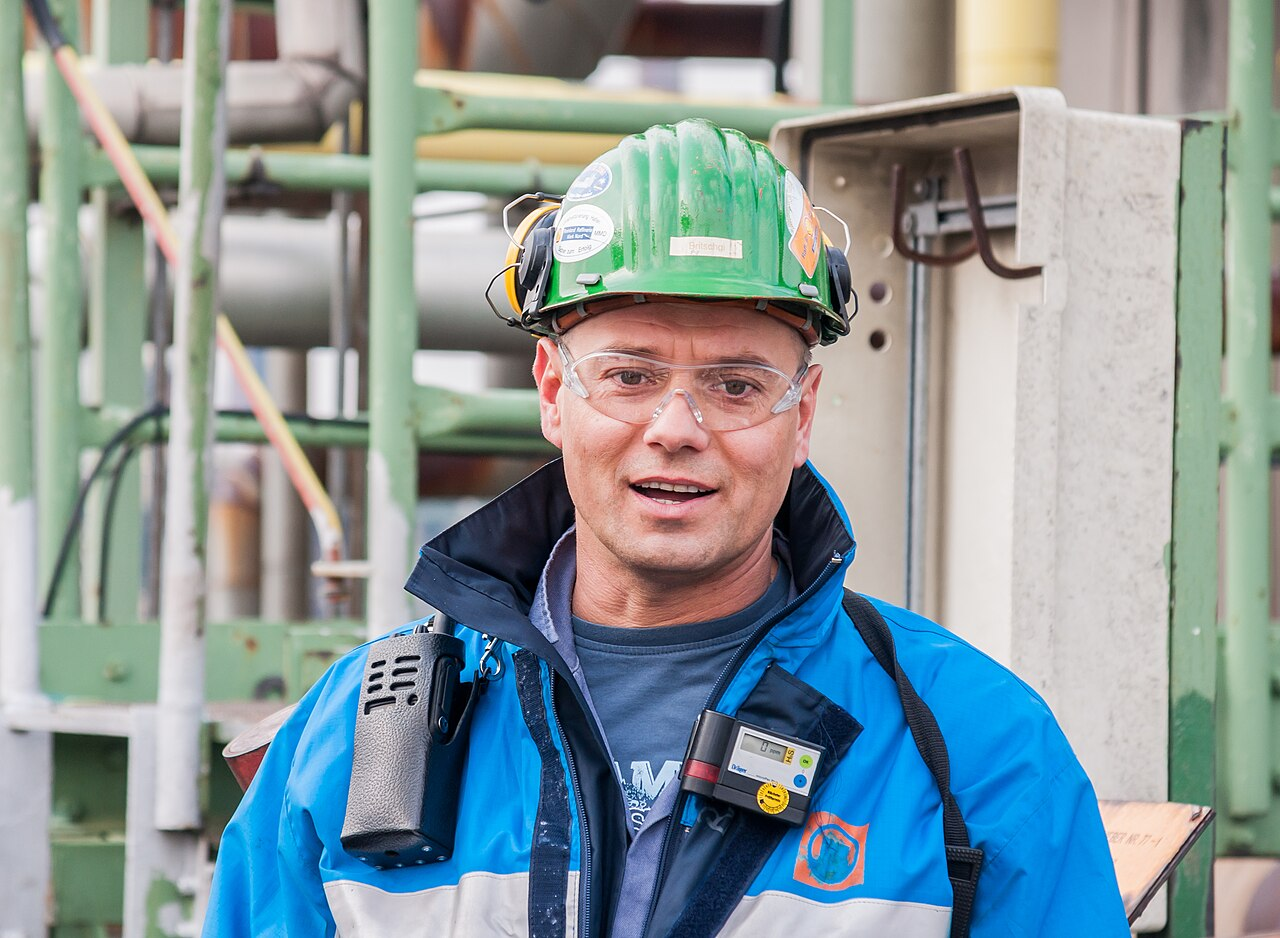
\includegraphics[width=\columnwidth, alt={Close up portrait of an industrial worker wearing personal protective equipment in front of facility piping. The worker wears a green hard hat with attached ear muffs, clear safety glasses, a blue jacket with a radio attached to the shoulder, and a portable gas detector clipped to the chest.}]{Cologne_Germany_Industrial-work-with-Personal-Protective-Equipment-04.jpg}
                
                {\tiny \textbf{Attribution:} Photo by CEphoto, Uwe Aranas, \href{https://creativecommons.org/licenses/by-sa/3.0}{CC BY-SA 3.0}, via \href{https://commons.wikimedia.org/wiki/File:Cologne_Germany_Industrial-work-with-Personal-Protective-Equipment-04.jpg}{Wikimedia Commons}\par}
            \end{figure}
        \end{column}
	\end{columns}
\end{frame}

\begin{frame}
    \frametitle{FR Clothing}
	\begin{columns}
	\begin{column}{0.48\linewidth}
		\begin{itemize}[<+- | alert@+>]
			\item{Must not continue to burn when ignited}
			\item{Must insulate well enough to dissipate heat away from skin}
			\item{Must resist the break open force of the shockwave}
		\end{itemize}
	\end{column}
	\begin{column}{0.48\linewidth}
            \begin{figure}
                \centering
                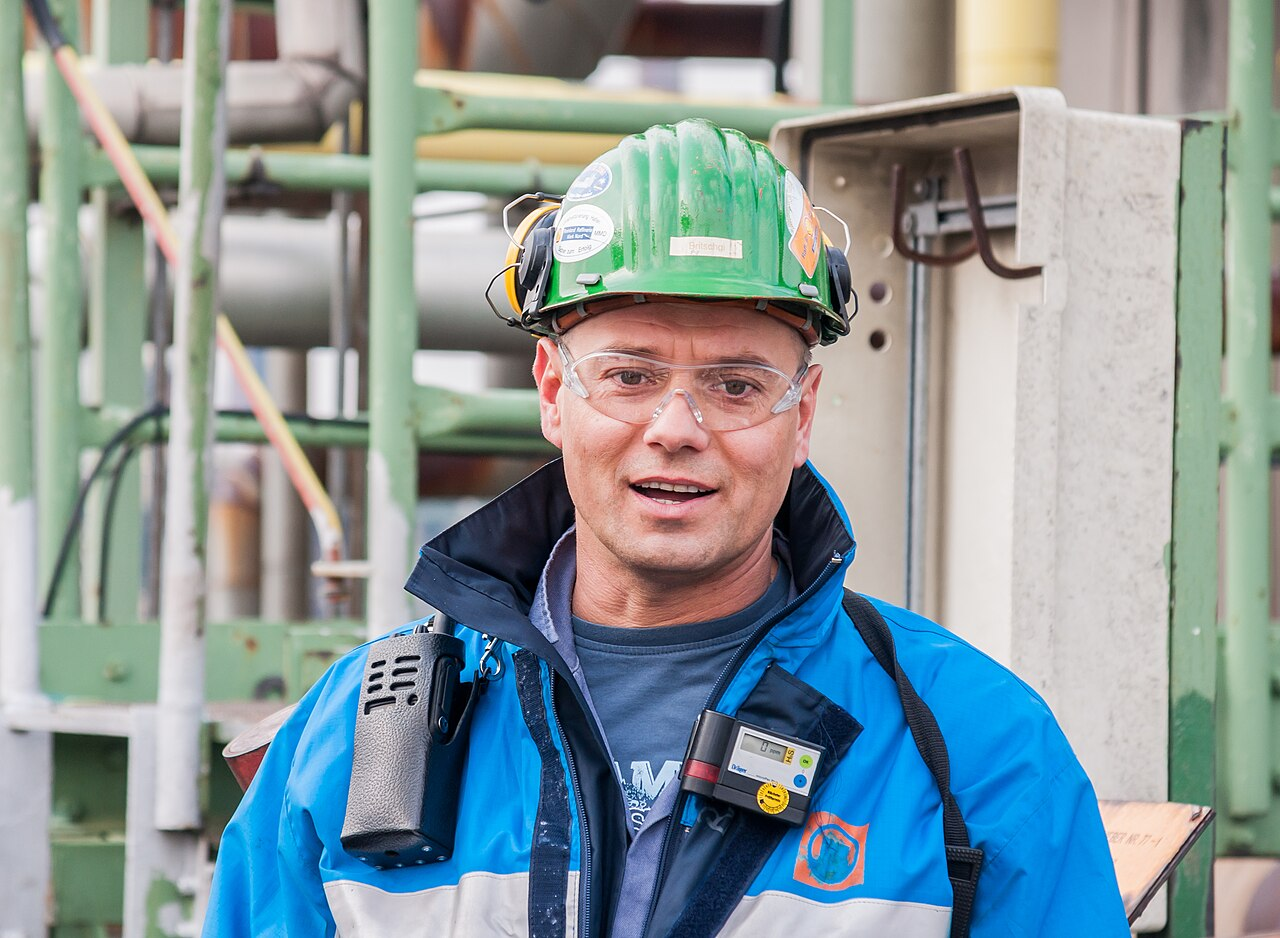
\includegraphics[width=\columnwidth, alt={Close up portrait of an industrial worker wearing personal protective equipment in front of facility piping. The worker wears a green hard hat with attached ear muffs, clear safety glasses, a blue jacket with a radio attached to the shoulder, and a portable gas detector clipped to the chest.}]{Cologne_Germany_Industrial-work-with-Personal-Protective-Equipment-04.jpg}
                
                {\tiny \textbf{Attribution:} Photo by CEphoto, Uwe Aranas, \href{https://creativecommons.org/licenses/by-sa/3.0}{CC BY-SA 3.0}, via \href{https://commons.wikimedia.org/wiki/File:Cologne_Germany_Industrial-work-with-Personal-Protective-Equipment-04.jpg}{Wikimedia Commons}\par}
            \end{figure}
	\end{column}
	\end{columns}
\end{frame}

\begin{frame}
    \frametitle{Eye Protection}
	\begin{columns}
	\begin{column}{0.48\linewidth}
		\begin{itemize}[<+- | alert@+>]
			\item{OSHA 29 CFR 1910.133 Eye and Face Protection}
			\item{Safety glasses}
			\item{Goggles}
			\item{Face shield}
			\item{Arc flash hood}
		\end{itemize}
	\end{column}
	\begin{column}{0.48\linewidth}
            \begin{figure}
                \centering
                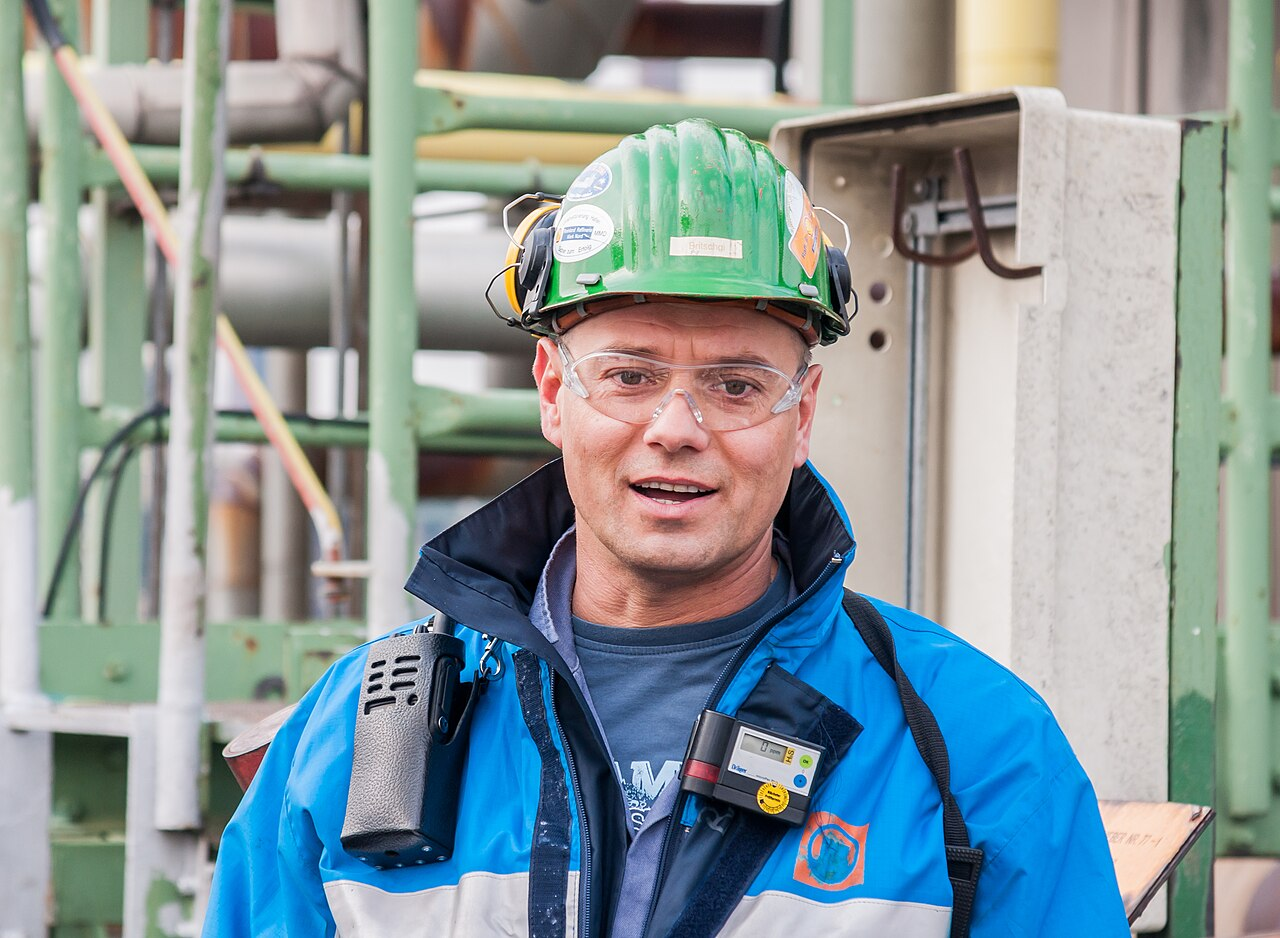
\includegraphics[width=\columnwidth, alt={Close up portrait of an industrial worker wearing personal protective equipment in front of facility piping. The worker wears a green hard hat with attached ear muffs, clear safety glasses, a blue jacket with a radio attached to the shoulder, and a portable gas detector clipped to the chest.}]{Cologne_Germany_Industrial-work-with-Personal-Protective-Equipment-04.jpg}
                
                {\tiny \textbf{Attribution:} Photo by CEphoto, Uwe Aranas, \href{https://creativecommons.org/licenses/by-sa/3.0}{CC BY-SA 3.0}, via \href{https://commons.wikimedia.org/wiki/File:Cologne_Germany_Industrial-work-with-Personal-Protective-Equipment-04.jpg}{Wikimedia Commons}\par}
            \end{figure}
	\end{column}
	\end{columns}
\end{frame}

\begin{frame}
    \frametitle{Hand Protection}

	\begin{columns}
        \begin{column}{0.48\linewidth}
            \begin{itemize}[<+- | alert@+>]
                \item{Live electrical work requires the use of rubber insulating gloves}
                \item{Leather gloves are worn \textbf{OVER} rubber gloves to protect the rubber}
                \item{Leather gloves \textbf{ARE NOT} a sufficient insulator alone}
            \end{itemize}
        \end{column}
        \begin{column}{0.48\linewidth}
            \begin{figure}
                \centering
                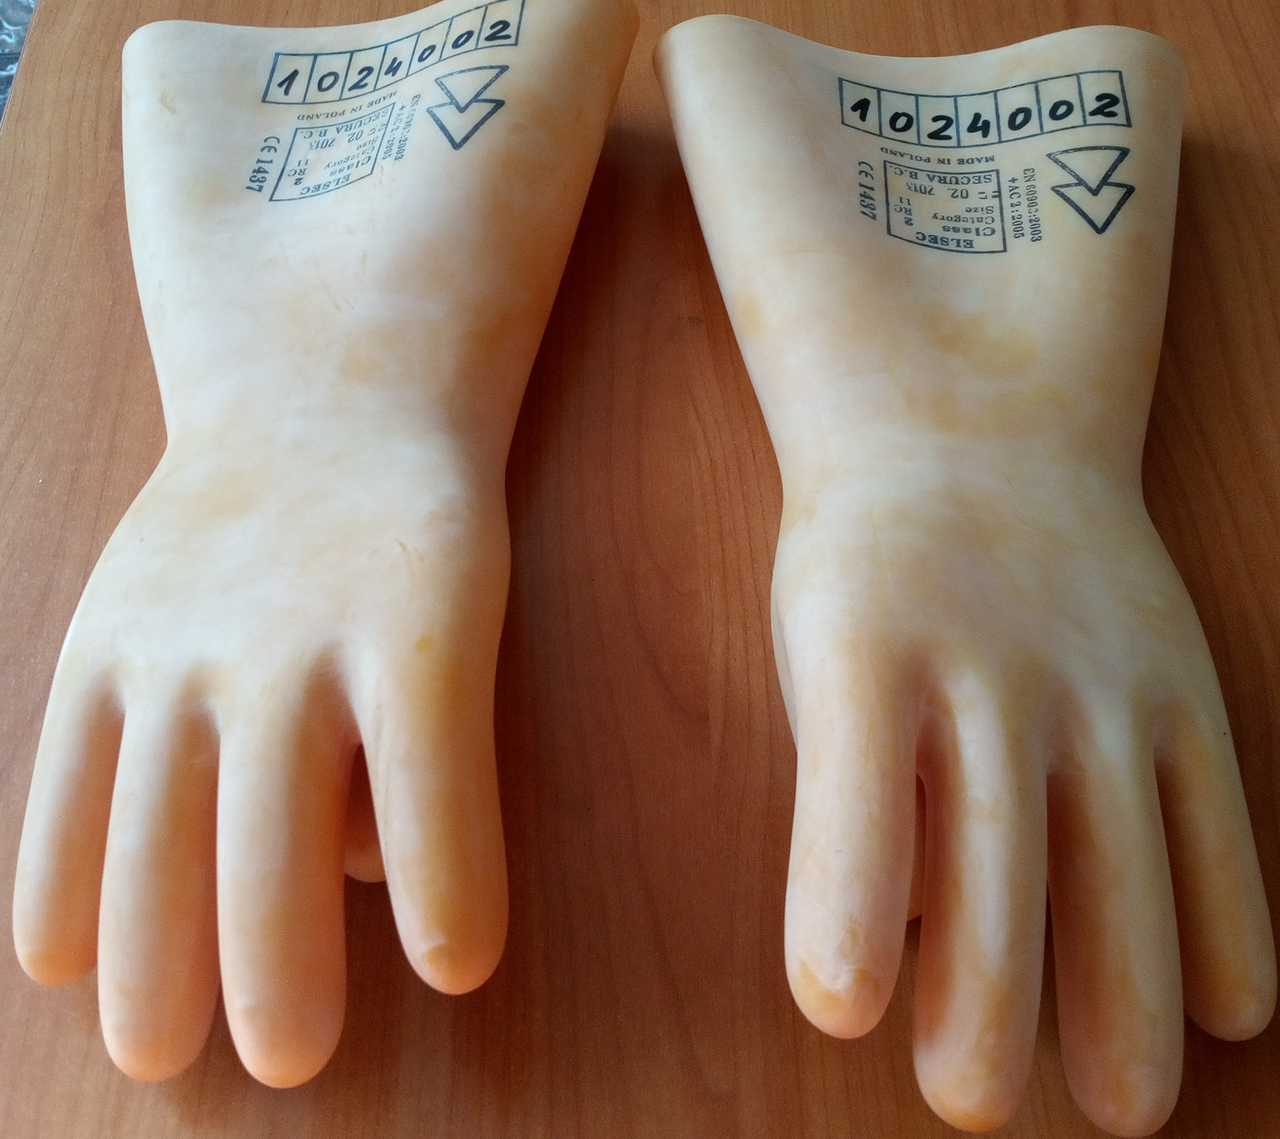
\includegraphics[width=\columnwidth, alt={}]{Electrical_safety_gloves.png}
                
                {\tiny \textbf{Attribution:} Powerfox, \href{https://creativecommons.org/licenses/by-sa/4.0}{CC BY-SA 4.0}, via \href{https://commons.wikimedia.org/wiki/File:Cologne_Germany_Industrial-work-with-Personal-Protective-Equipment-04.jpg}{Wikimedia Commons}\par}
            \end{figure}
        \end{column}
	\end{columns}
\end{frame}

% \begin{frame}
%     \frametitle{Hand Protection}
% 	\begin{figure}
% 		\centering
% 		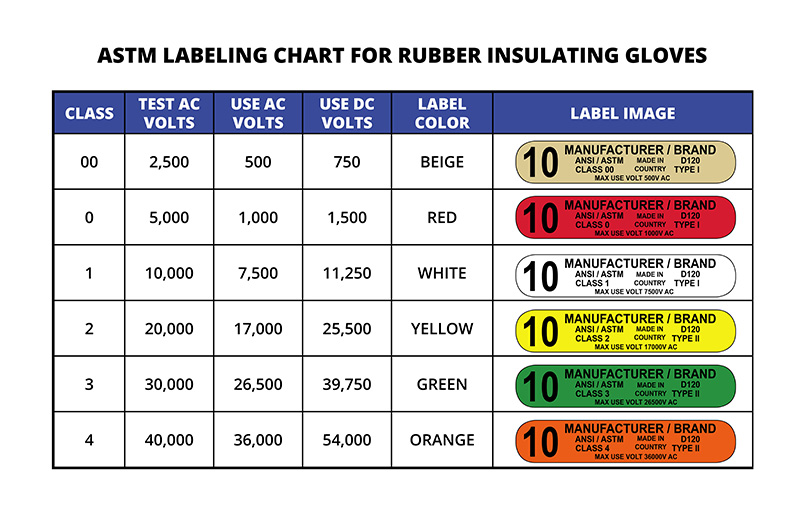
\includegraphics[width=0.75\columnwidth]{glovechart}
% 		\caption*{ASTM D 120-2 defines a voltage rating and color code for insulating gloves}
% 		%\label{fig:Burns1}
% 	\end{figure}
% \end{frame}

\begin{frame}
    \frametitle{Personal Protective Equipment}

    \centering
    \href{https://www.yout-ube.com/watch?v=nw_pNMnLG3A}{PPE SAFETY VIDEO | Testing common types of PPE} (3:48)  

    {\scriptsize \href{https://www.yout-ube.com/watch?v=nw_pNMnLG3A}{https://www.yout-ube.com/watch?v=nw\_pNMnLG3A}}
\end{frame}

\subsection{Lockout/Tagout}

\begin{frame}
    \frametitle{Control of Hazardous Energy}

	\begin{columns}
        \begin{column}{0.48\linewidth}
            \begin{itemize}[<+- | alert@+>]
                \item{OSHA 29 CFR 1910.147 Control of Hazardous Energy}
                \begin{itemize}
                    \item{Note: \textbf{ENERGY} -- LOTO is not limited to electricity}
                \end{itemize}
                \item{LOTO should be carried out whenever any piece of equipment is being serviced, repaired, or replaced}
            \end{itemize}
        \end{column}
        \begin{column}{0.48\linewidth}
            \begin{figure}
                \centering
                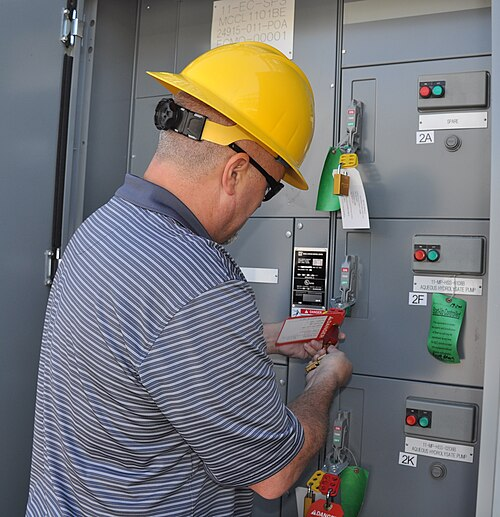
\includegraphics[width=0.75\columnwidth, alt={Worker wearing a bright yellow hard hat and glasses applying a red lockout tagout device to an electrical switchboard panel. The grey industrial panel features multiple switch compartments labeled with numbers, buttons, green inspection tags, and brass padlocks.}]{Blue_Grass_Lockout.jpg}
                
                {\tiny \textbf{Attribution:} Powerfox, \href{https://creativecommons.org/licenses/by-sa/4.0}{CC BY-SA 4.0}, via \href{https://commons.wikimedia.org/wiki/File:Cologne_Germany_Industrial-work-with-Personal-Protective-Equipment-04.jpg}{Wikimedia Commons}\par}
            \end{figure}
        \end{column}
	\end{columns}
\end{frame}

\begin{frame}
    \frametitle{Lockout/Tagout}

	\begin{columns}
        \begin{column}{0.48\linewidth}
            \begin{enumerate}[<+- | alert@+>]
                \item{Prepare for shutdown}
                \item{Shut down}
                \item{Isolate power sources}
                \item{LOTO power sources}
                \item{Release stored energy}
                \item{Verify isolation}
            \end{enumerate}
        \end{column}
        \begin{column}{0.48\linewidth}
            \begin{figure}
                \centering
                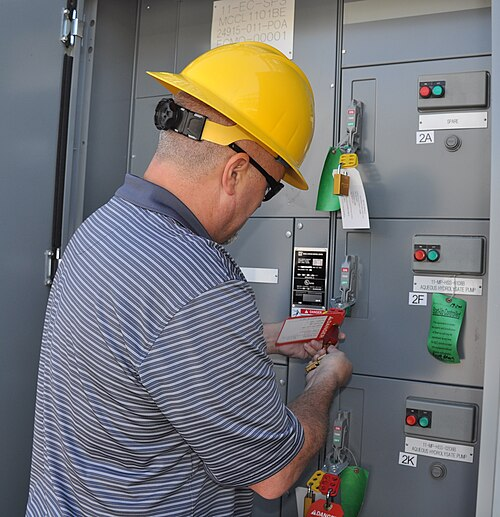
\includegraphics[width=0.75\columnwidth, alt={Worker wearing a bright yellow hard hat and glasses applying a red lockout tagout device to an electrical switchboard panel. The grey industrial panel features multiple switch compartments labeled with numbers, buttons, green inspection tags, and brass padlocks.}]{Blue_Grass_Lockout.jpg}
                
                {\tiny \textbf{Attribution:} Powerfox, \href{https://creativecommons.org/licenses/by-sa/4.0}{CC BY-SA 4.0}, via \href{https://commons.wikimedia.org/wiki/File:Cologne_Germany_Industrial-work-with-Personal-Protective-Equipment-04.jpg}{Wikimedia Commons}\par}
            \end{figure}
        \end{column}
	\end{columns}
\end{frame}

\begin{frame}
    \frametitle{Why LOTO Is So Important}

    \centering
	\href{https://www.yout-ube.com/watch?v=cNcsTRQNZLE}{First Day on the Job Was His Last: What Happened to Day Davis} (2:50) 

    {\scriptsize \href{https://www.yout-ube.com/watch?v=cNcsTRQNZLE}{https://www.yout-ube.com/watch?v=cNcsTRQNZLE}}
\end{frame}

\begin{frame}
    \frametitle{Copyright Notice}

    \begin{figure}
        \centering
        
\includegraphics[width=0.625\linewidth, alt={Creative Commons Attribution NonCommercial ShareAlike logo displaying four circular icons arranged horizontally over a black banner. From left to right, the icons feature the CC logo, a person pictogram for Attribution labeled BY below, a slashed dollar sign for NonCommercial labeled NC below, and a counterclockwise circular arrow for ShareAlike labeled SA below.}]{by-nc-sa.png}
    \end{figure}

    \vspace{0.5em}
    \centering
    Electricity and Electrical Safety \textcopyright 2026 by Brad Peirson is licensed under \href{https://creativecommons.org/licenses/by-nc-sa/4.0/}{CC BY-NC-SA 4.0}. To view a copy of this license, visit \href{https://creativecommons.org/licenses/by-nc-sa/4.0/}{https://creativecommons.org/licenses/by-nc-sa/4.0/}
\end{frame}

\end{document}

% \begin{frame}
%     \frametitle{Test Todo}

%     % Usage: \tikztodo[width]{height}{description/notes}
%     \tikztodo[0.7\textwidth]{4cm}{Convert block diagram of feedback loop}
% \end{frame}